\chapter{Analisi sperimentale}
\label{cha:AnalisiSperimentale}

Il presente capitolo è dedicato all'analisi dei dati raccolti per i demoni
\texttt{\textbf{NTPsec}}, \texttt{\textbf{ptp4l}} e \texttt{\textbf{Chronyd}}, con
l'obiettivo di valutarne il comportamento al variare delle condizioni di rete introdotte
nei tre scenari sperimentali. L'attenzione è rivolta all'esame delle principali
metriche di sincronizzazione temporale osservate durante la fase di testing, al fine
di evidenziare l'impatto del progressivo incremento degli impairment di rete sulla
stabilità del sistema e sulla qualità del processo di sincronizzazione.

Per ciascuna metrica di interesse non è stata considerata una singola esecuzione,
bensì un insieme di run indipendenti, ottenute ripetendo più volte la medesima procedura
sperimentale. Di conseguenza, i grafici e le statistiche riportati nel seguito non
descrivono l'andamento di una sola acquisizione, ma una sintesi aggregata delle
diverse run effettuate.

L'analisi è organizzata per metrica. Per ciascuna grandezza considerata viene condotto
un confronto sistematico tra i tre scenari sperimentali definiti in precedenza,
corrispondenti a differenti livelli di degrado della rete (\texttt{low}, \texttt{medium},
\texttt{high}). L'aggregazione dei dati è stata effettuata allineando i campioni
omologhi delle diverse run rispetto all'indice di campionamento, così da rendere confrontabili
tra loro le varie esecuzioni anche in presenza di leggere differenze temporali nella
raccolta.

Per ogni metrica sono stati costruiti due differenti tipi di rappresentazione grafica.
Nel primo caso, la curva centrale rappresenta la media dei valori osservati tra le
run, mentre la banda associata corrisponde all'intervallo di confidenza al 95\%,
fornendo una misura della stabilità della stima media ottenuta. Nel secondo caso,
la curva centrale rimane la media aggregata, ma le bande descrivono direttamente la
dispersione empirica dei dati: la banda interna rappresenta l'intervallo
inter-quartile, compreso tra primo e terzo quartile, mentre la banda esterna
rappresenta l'intervallo tra il decimo e il novantesimo percentile. I due grafici
risultano quindi complementari: il primo è utile per valutare quanto la media
osservata sia statisticamente stabile tra le run, mentre il secondo consente di apprezzare
con maggiore immediatezza la variabilità effettiva dei valori misurati e la presenza
di eventuali oscillazioni o dispersioni marcate.

Nel seguito, l'interpretazione delle metriche verrà svolta confrontando i tre
scenari sperimentali sia in termini di livello medio delle grandezze osservate, sia
in termini di variabilità, robustezza e regolarità del comportamento dei diversi
demoni di sincronizzazione.

Nella discussione dei risultati verrà attribuito particolare rilievo ai grafici
con intervallo inter-quartile e banda p10--p90, in quanto più adatti a
rappresentare la dispersione effettiva delle osservazioni aggregate.

\begin{table}[H]
  \centering
  \caption{Matrice di scenario - fase 3 (topologia T2 + tc/netem)}
  \begin{tabular}{|c|c|c|c|c|c|}
    \hline
    \textbf{Scenario} & \textbf{Delay} & \textbf{Jitter} & \textbf{Loss} & \textbf{Reorder} & \textbf{Rate Limit} \\
    \hline
    \texttt{LOW}      & 5 ms           & 1 ms            & 0.1\%         & 1\%              & 50 Mbit             \\
    \hline
    \texttt{MEDIUM}   & 15 ms          & 5 ms            & 0.5\%         & 5\%              & 20 Mbit             \\
    \hline
    \texttt{HIGH}     & 60 ms          & 20 ms           & 10\%          & 20\%             & 5 Mbit              \\
    \hline
  \end{tabular}
  \label{tab:scenario_matrix}
\end{table}
\section{\texttt{NTPsec}}

Nel caso di \texttt{\textbf{NTPsec}}, l'analisi si concentra su tre metriche principali:
\texttt{\textbf{delay}}, \texttt{\textbf{jitter}} e \texttt{\textbf{offset}}. Queste
grandezze permettono di caratterizzare, rispettivamente, sia il tempo di propagazione
dei pacchetti NTP, sia la variabilità temporale delle misurazioni e lo
scostamento tra il clock locale e il clock di riferimento. L'evoluzione nei diversi
scenari permette di valutare la robustezza del demone rispetto al degrado delle condizioni
di rete e di analizzare la qualità del processo di sincronizzazione in termini sia
di stabilità sia di accuratezza.

I dati oggetto dell'analisi sono stati raccolti secondo la metodologia sperimentale
illustrata nei capitoli precedenti. In questa sede non saranno quindi ripresi
gli aspetti relativi alla configurazione dell'ambiente di prova o alla
disposizione della topologia. Nel caso di \texttt{\textbf{NTPsec}}, le misurazioni
considerate sono state rilevate sui nodi \texttt{clientntp} e \texttt{boundary} della
topologia, in coerenza con il ruolo da essi ricoperto nel processo di
sincronizzazione.

Ciascuna sezione seguente è quindi dedicata a una singola metrica e presenta, per
i tre scenari sperimentali, i risultati osservati e il relativo confronto
interpretativo, con l'obiettivo di individuare eventuali differenze significative
tra le condizioni di rete considerate e valutarne gli effetti sul comportamento del
demone.

\subsection{\texttt{clientntp}}
L'analisi effettuata sul nodo \texttt{clientntp} è caratterizzata da uno stato
di inizializzazione, identificato da \texttt{refid=.INIT.}, \texttt{stratum=16}, \texttt{selected=False}
e \texttt{reach=0}. L'intervallo non è rappresentativo del regime operativo
della sincronizzazione, pertanto non viene considerato nel confronto tra scenari,
il quale viene condotto a partire dal primo campione valido. Ai fini interpretativi,
l'attenzione è principalmente rivolta alla porzione \texttt{post-selected} della serie,
cioè ai campioni successivi alla selezione del peer di riferimento.
\subsubsection{Analisi metrica: \texttt{delay}}
\begin{figure}[H]
  \centering

  \begin{subfigure}
    {0.32\textwidth}
    \centering
    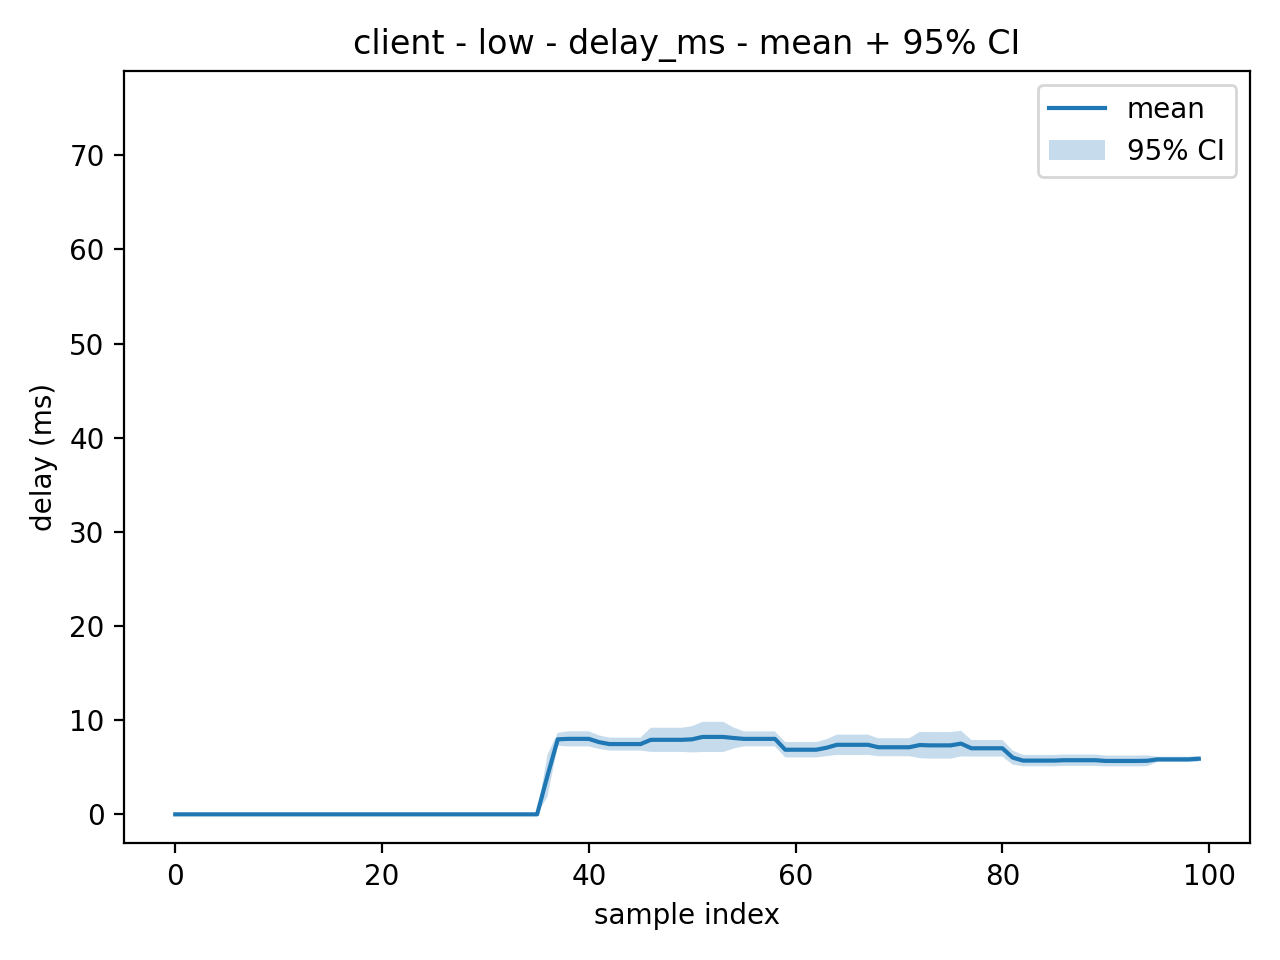
\includegraphics[width=\linewidth]{
      pars_plots/ntpsec/_aggregated/client/low/delay_ms_mean_ci95.png
    }
    \caption{Scenario LOW}
  \end{subfigure}
  \hfill
  \begin{subfigure}
    {0.32\textwidth}
    \centering
    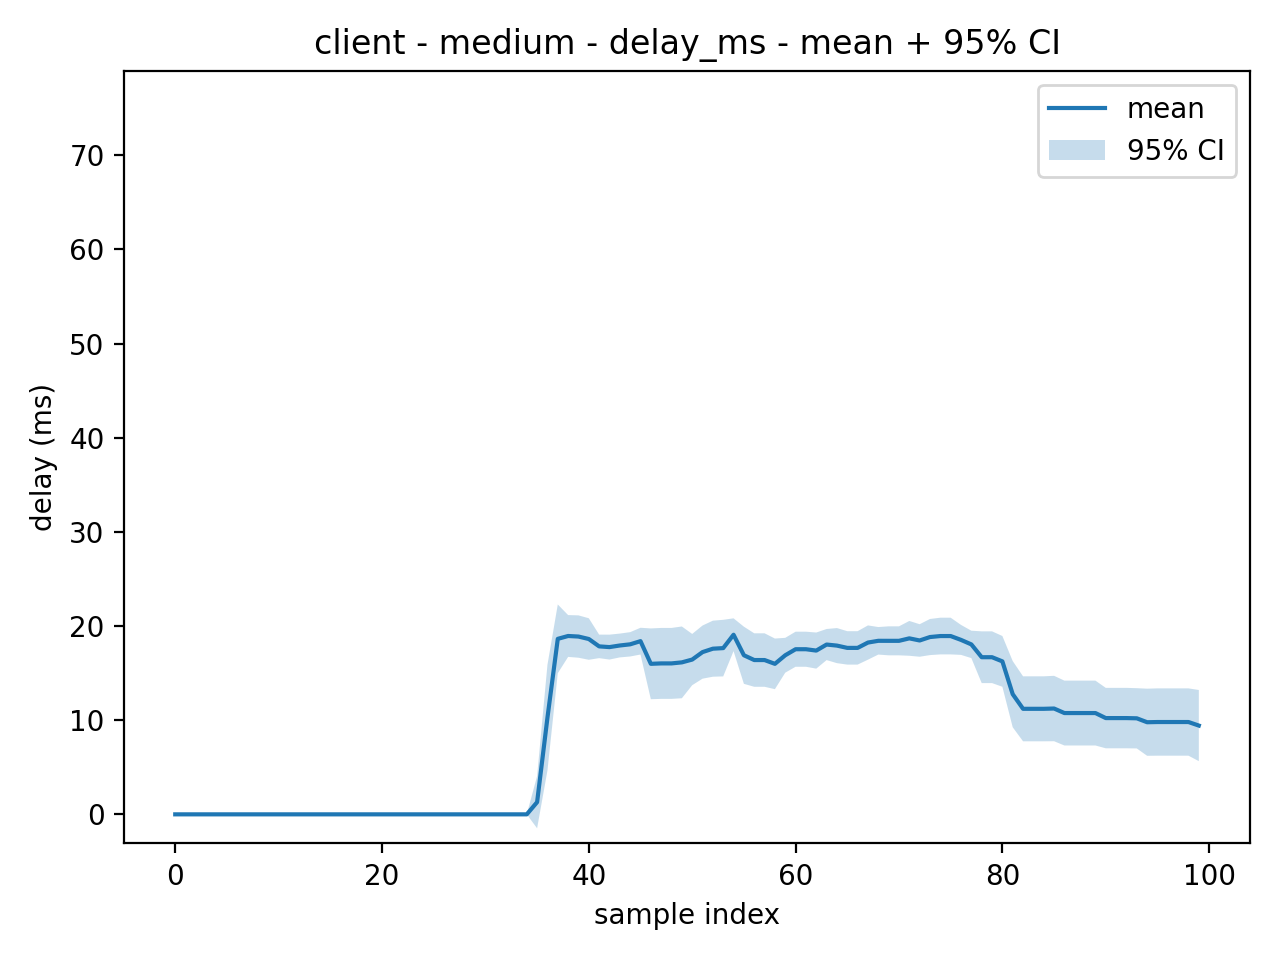
\includegraphics[width=\linewidth]{
      pars_plots/ntpsec/_aggregated/client/medium/delay_ms_mean_ci95.png
    }
    \caption{Scenario MEDIUM}
  \end{subfigure}
  \hfill
  \begin{subfigure}
    {0.32\textwidth}
    \centering
    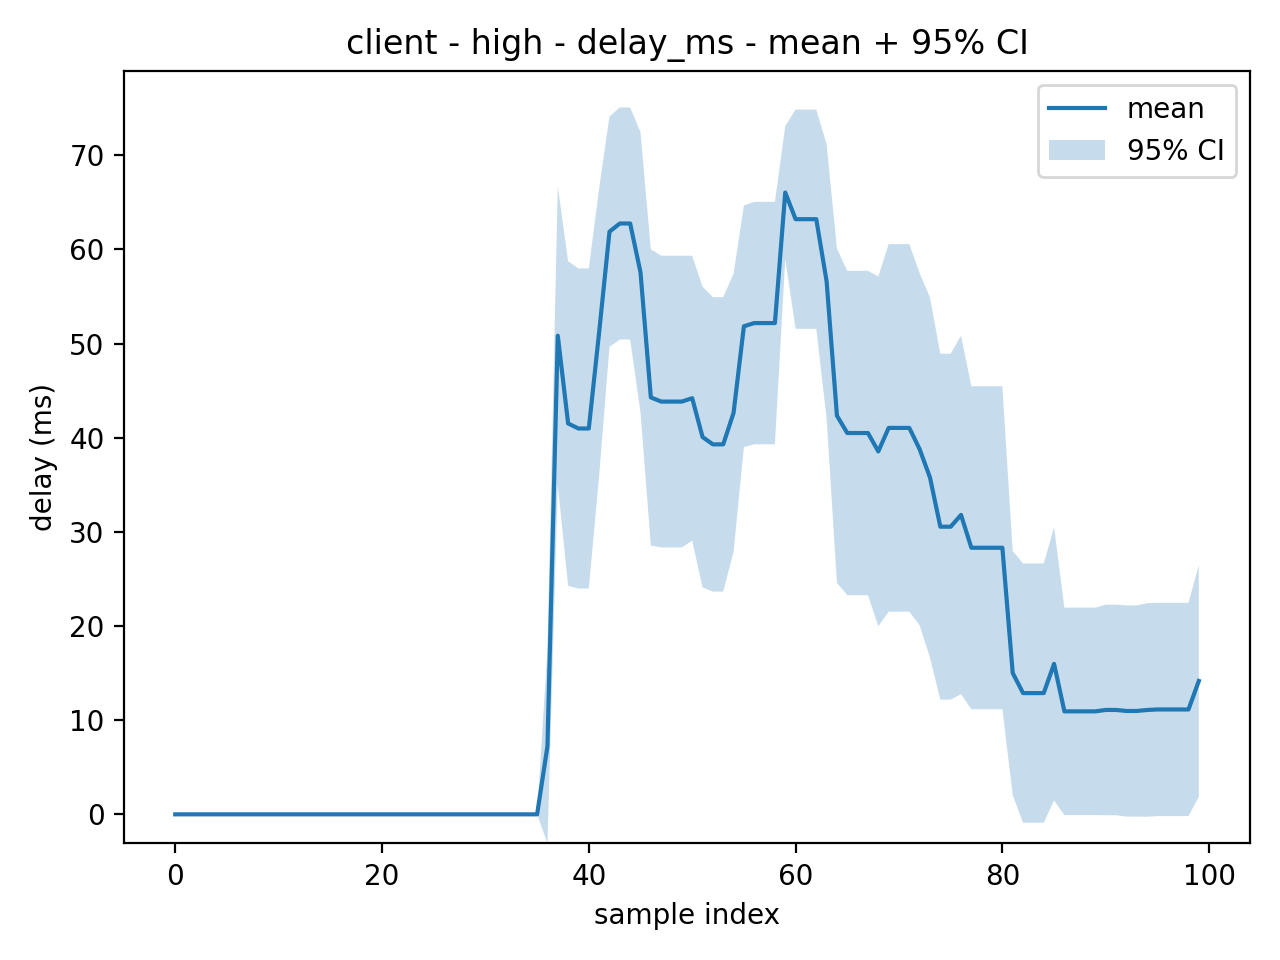
\includegraphics[width=\linewidth]{
      pars_plots/ntpsec/_aggregated/client/high/delay_ms_mean_ci95.png
    }
    \caption{Scenario HIGH}
  \end{subfigure}

  \caption{Media con intervallo di confidenza al 95\% - nodo: \texttt{clientntp}}
  \label{fig:scenario_comparison}
\end{figure}
\begin{figure}[H]
  \centering

  \begin{subfigure}
    {0.32\textwidth}
    \centering
    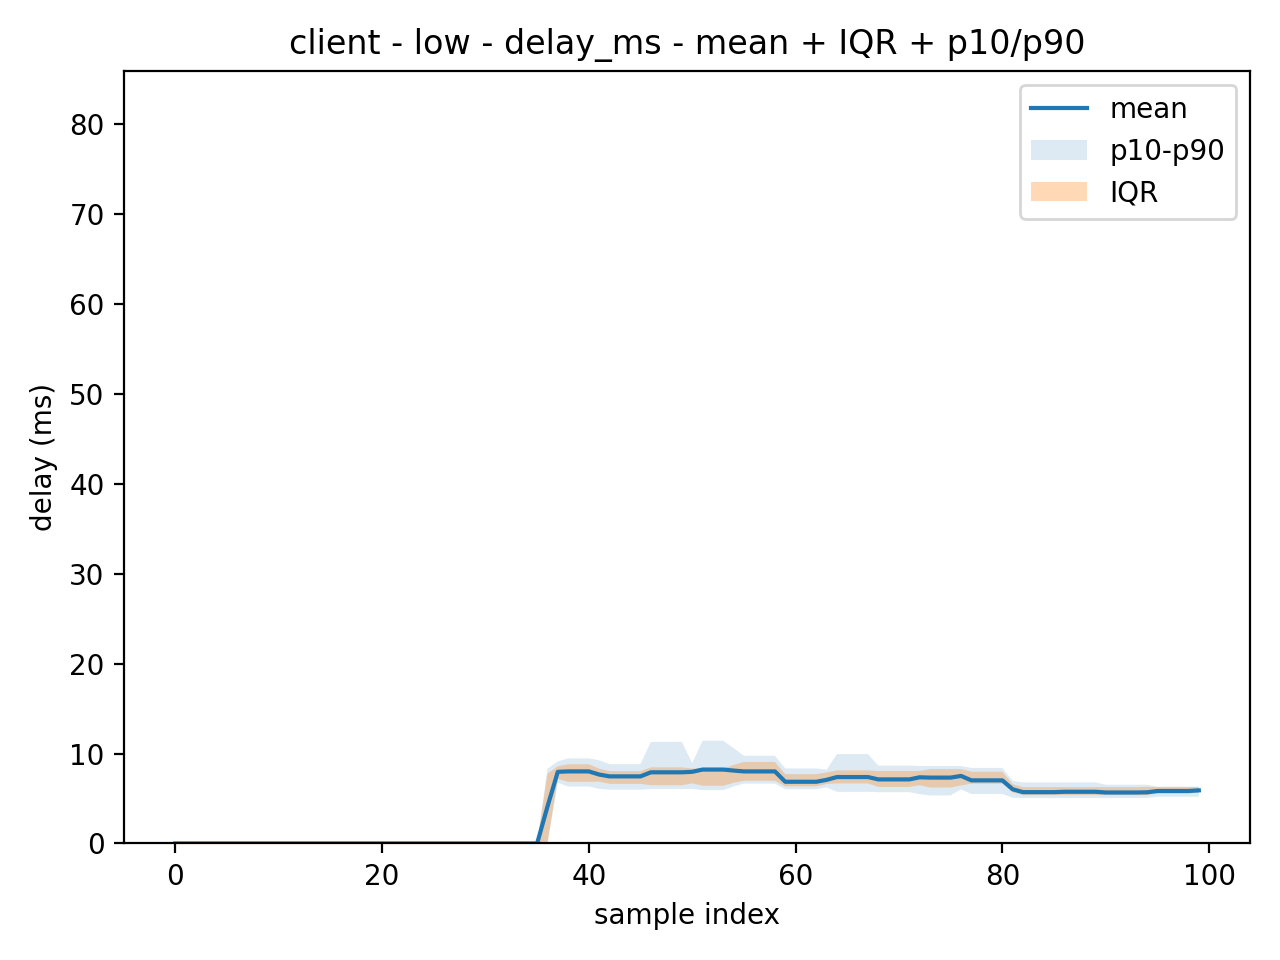
\includegraphics[width=\linewidth]{
      pars_plots/ntpsec/_aggregated/client/low/delay_ms_mean_iqr_p10_p90.png
    }
    \caption{Scenario LOW}
  \end{subfigure}
  \hfill
  \begin{subfigure}
    {0.32\textwidth}
    \centering
    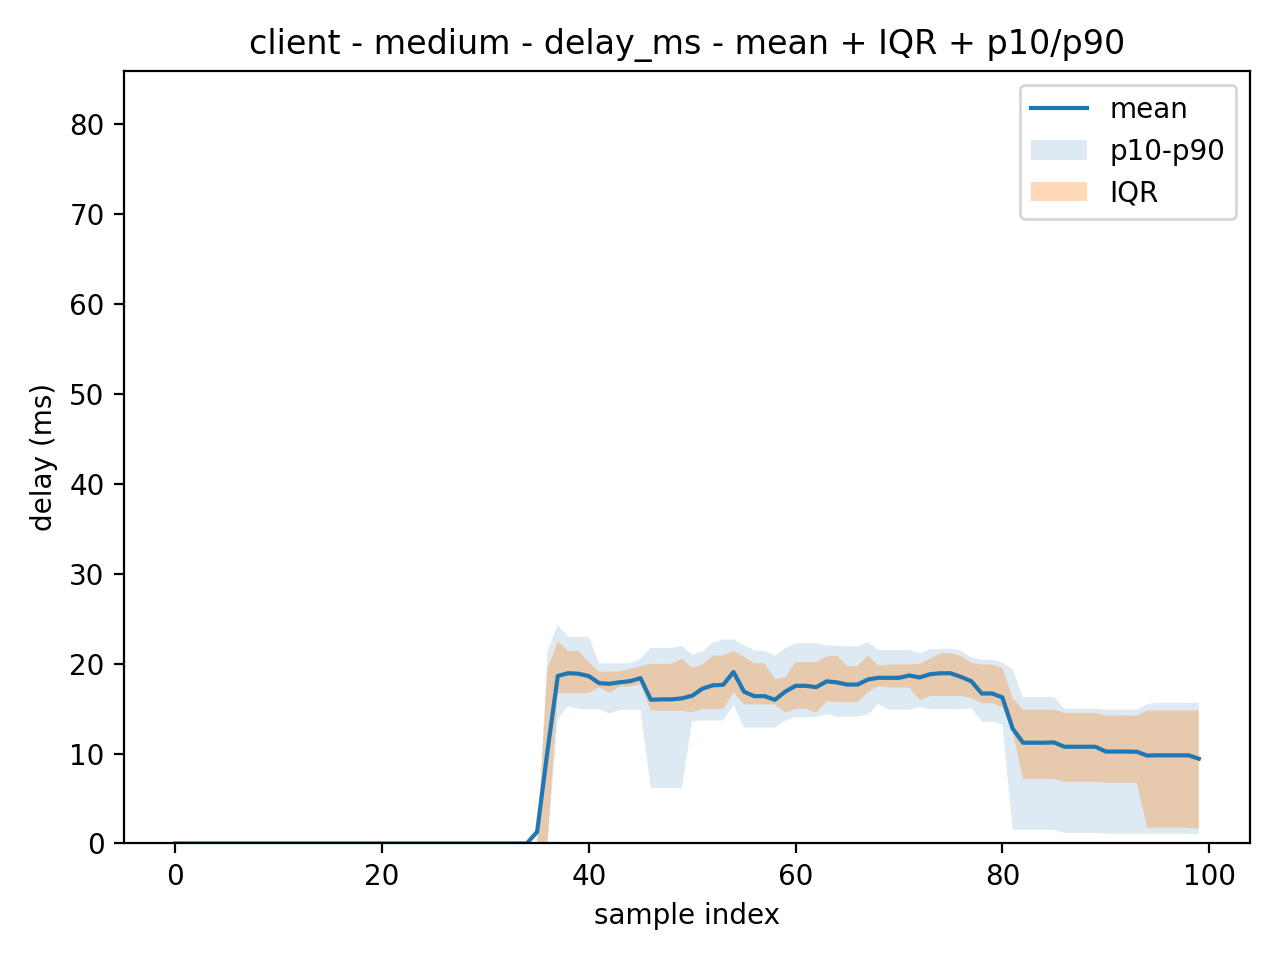
\includegraphics[width=\linewidth]{
      pars_plots/ntpsec/_aggregated/client/medium/delay_ms_mean_iqr_p10_p90.png
    }
    \caption{Scenario MEDIUM}
  \end{subfigure}
  \hfill
  \begin{subfigure}
    {0.32\textwidth}
    \centering
    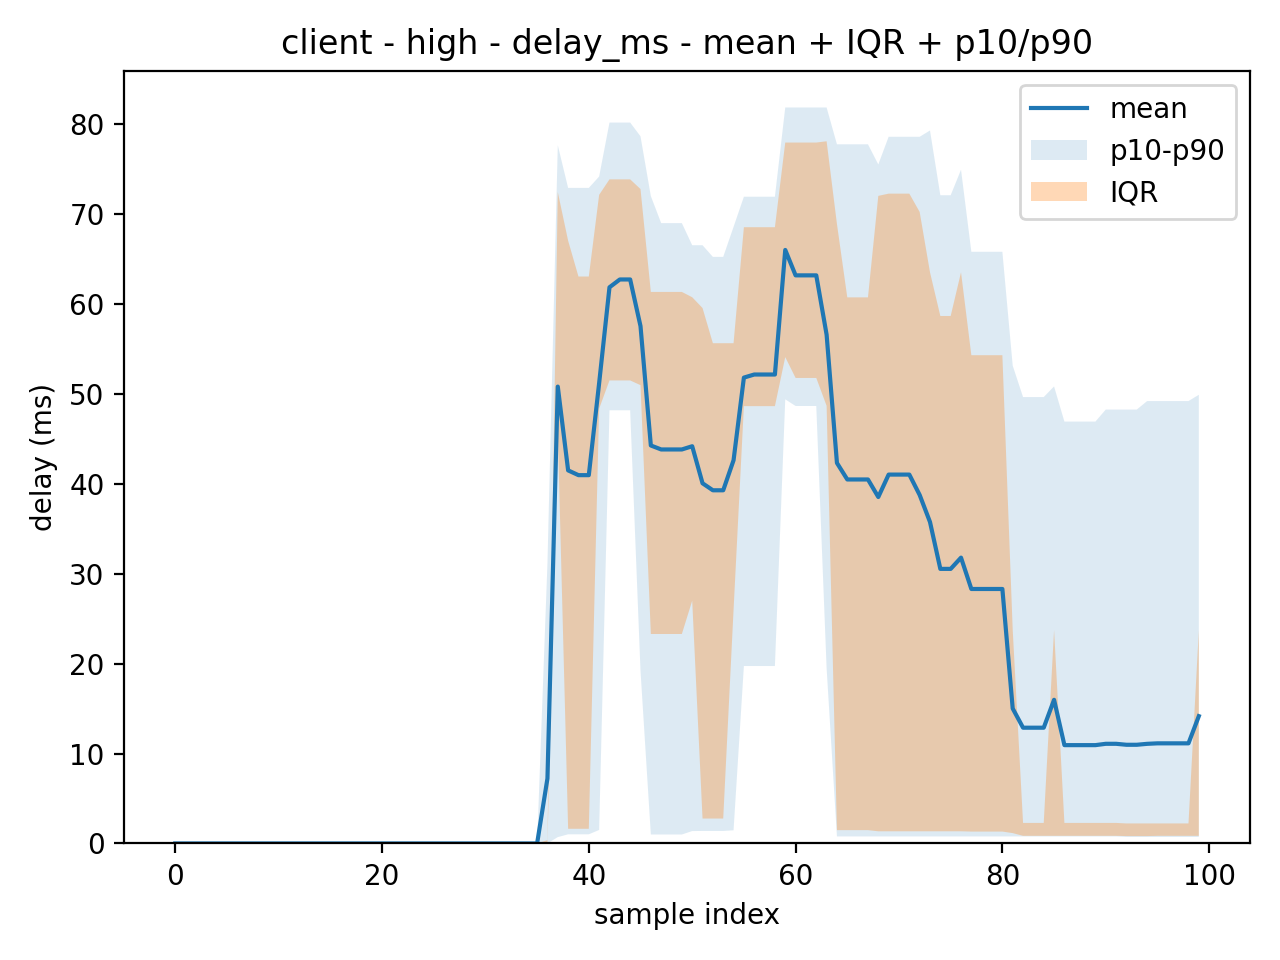
\includegraphics[width=\linewidth]{
      pars_plots/ntpsec/_aggregated/client/high/delay_ms_mean_iqr_p10_p90.png
    }
    \caption{Scenario HIGH}
  \end{subfigure}

  \caption{Media con banda inter-quartile e banda p10-p90 - nodo: \texttt{clientntp}}
  \label{fig:scenario_comparison}
\end{figure}

L'analisi del delay misurato sul nodo \texttt{clientntp} per il demone \texttt{NTPsec}
mette in evidenza una dipendenza dagli impairment di rete introdotte nei tre
scenari.

Nello scenario \texttt{low}, il delay assume valori contenuti e presenta un
andamento sostanzialmente regolare. La curva media si colloca stabilmente in una fascia
di circa 6–8 ms, con oscillazioni sufficientemente moderate con delle bande di
dispersione relativamente strette. Il delay medio è circa 7.00 ms, con una
mediana 6.82 ms e un intervallo inter-quartile uguale ~1.95 ms. La media della
banda inter-quartile di circa 1.43 ms, invece la larghezza media della banda p10–p90
è di circa 2.85 ms.

Nel caso \texttt{medium}, il delay cresce e si posiziona in una fascia superiore rispetto
al caso precedente. La curva media è nell'intervallo (16-19) ms per una parte
consistente dell'osservazione, per poi diminuire in fase finale verso valori ~10
ms. Il delay medio è ~15.5 ms, con mediana 16.5 ms e un intervallo inter-quartile di
~5.18 ms. L'IQR lungo la curva è ~5.62 ms e la p10–p90 ~10.0 ms.
Complessivamente l'andamento rimane leggibile e non ha instabilità estrema, evidenziando
comunque un peggioramento generale.

Nello scenario \texttt{high} si ha un comportamento con più degrado e meno
regolare. Post peer-selection, la curva media si posiziona in fase iniziale su
valori molto elevati, spesso compresi tra ~(40-65) ms, con oscillazioni ampie e una
forte eterogeneità tra run, evidenziato dall'ampliamento delle bande di
dispersione. Il livello medio è verso valori ~(10–15) ms. Il delay medio è pari a ~35.0
ms, con mediana 46.7 ms e l'intervallo inter-quartile molto ampio, pari a ~59.9 ms.
Le statistiche della curva aggregata confermano il trend, infatti si ha una
larghezza media della banda IQR è ~31.0 ms e quella p10–p90 ~59.4 ms.

Nel confronto tra scenari si evidenzia una progressione complessivamente coerente
con l'aumento della severità degli impairment di rete. Da \texttt{low} a \texttt{medium},
il delay del client cresce e contestualmente anche la sua dispersione,
mantenendo una dinamica ancora sufficientemente controllata. Nello scenario \texttt{high}
si evidenzia una maggiore discontinuità. Il livello medio è spostato su valori più
alti e lo stesso comportamento vale per la variabilità. Qualitativamente, la metrica
del delay risulta quindi efficace nel differenziare i tre scenari e nel mostrare come
l'incremento del degrado di rete si traduca in un peggioramento sia del livello della
misura sia della sua regolarità temporale.

\subsubsection{Analisi metrica: \texttt{jitter}}
\begin{figure}[H]
  \centering

  \begin{subfigure}
    {0.32\textwidth}
    \centering
    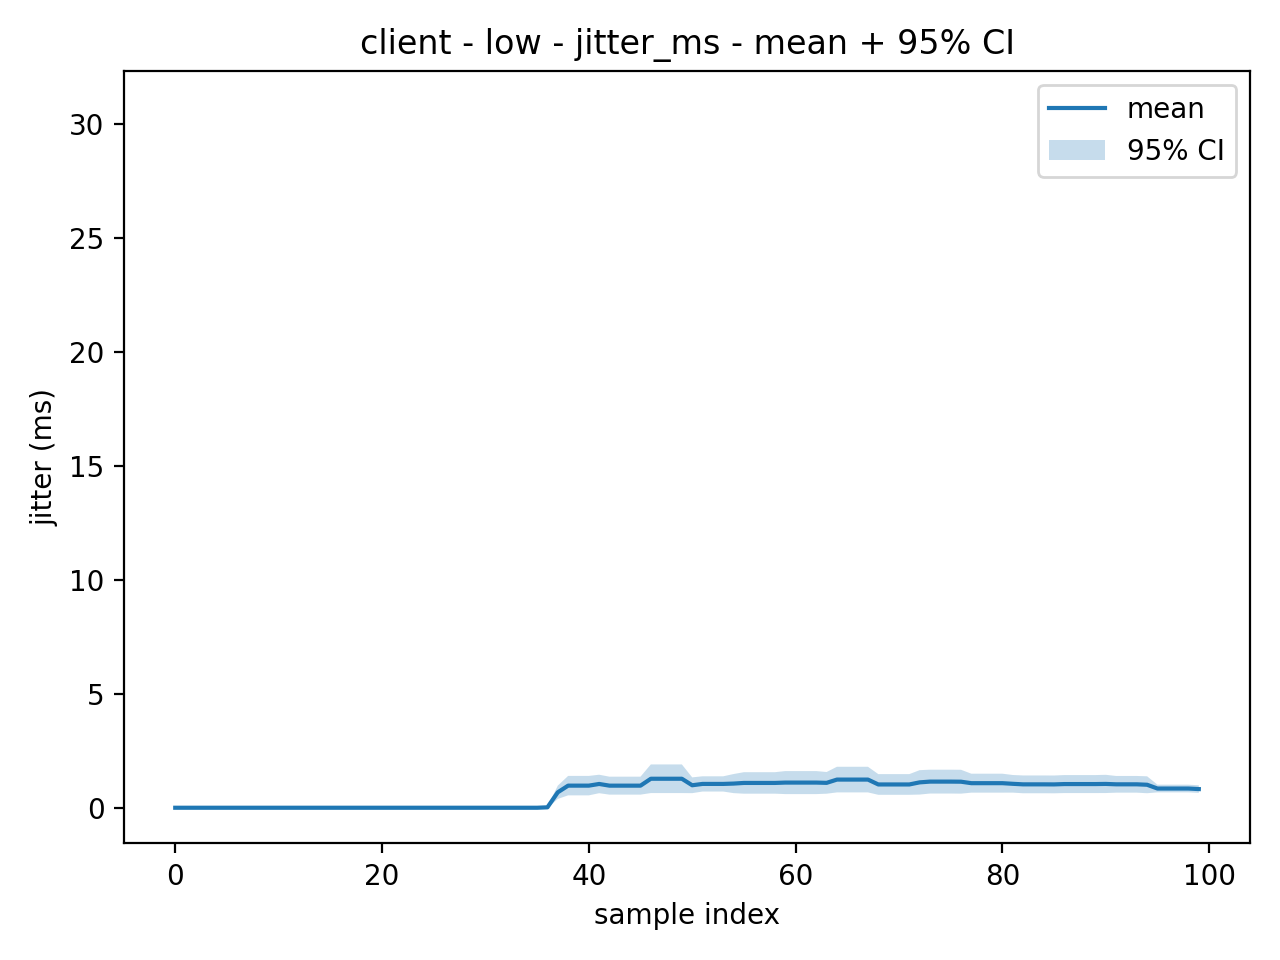
\includegraphics[width=\linewidth]{
      pars_plots/ntpsec/_aggregated/client/low/jitter_ms_mean_ci95.png
    }
    \caption{Scenario LOW}
  \end{subfigure}
  \hfill
  \begin{subfigure}
    {0.32\textwidth}
    \centering
    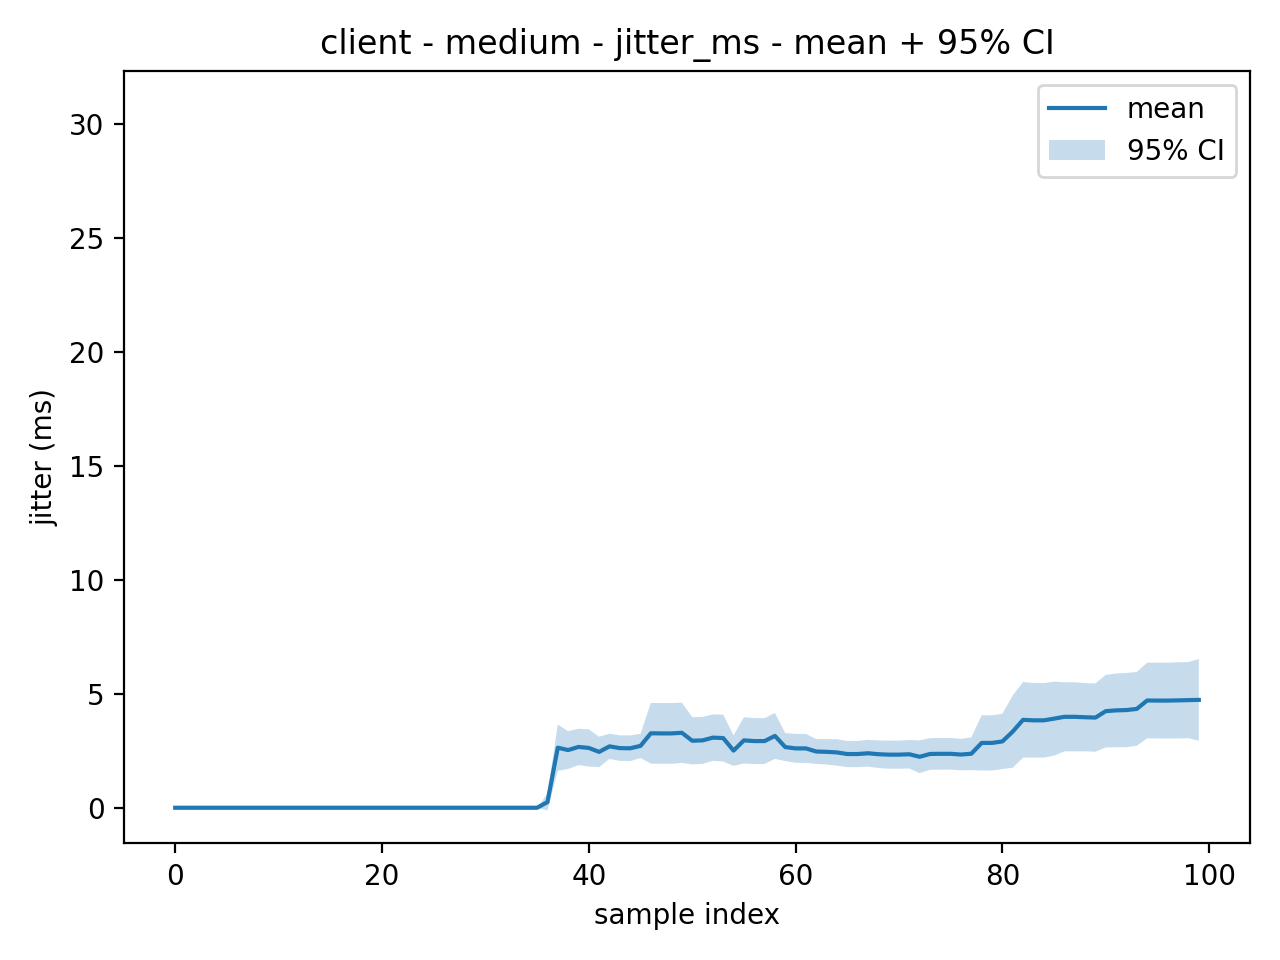
\includegraphics[width=\linewidth]{
      pars_plots/ntpsec/_aggregated/client/medium/jitter_ms_mean_ci95.png
    }
    \caption{Scenario MEDIUM}
  \end{subfigure}
  \hfill
  \begin{subfigure}
    {0.32\textwidth}
    \centering
    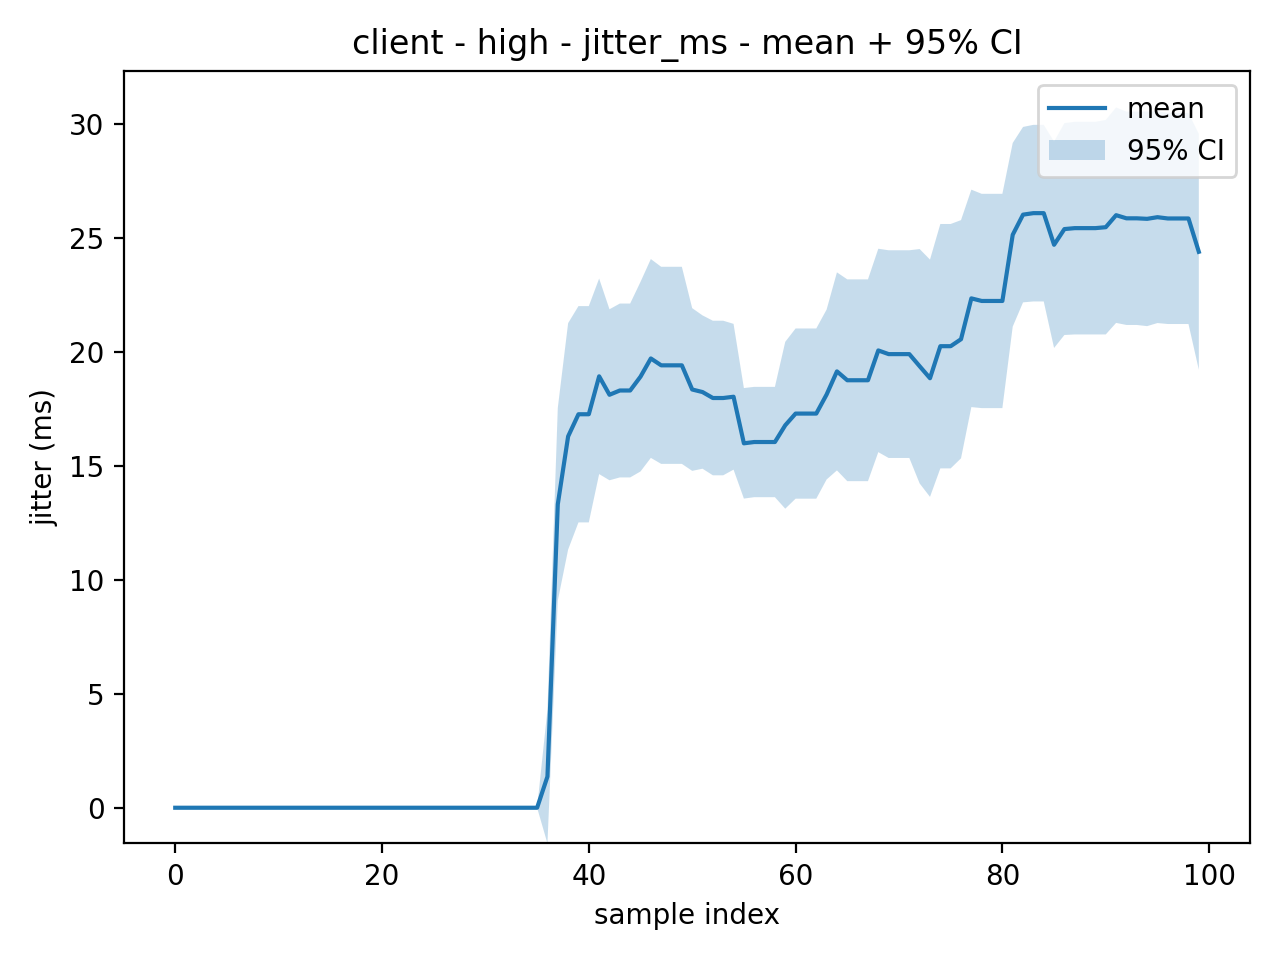
\includegraphics[width=\linewidth]{
      pars_plots/ntpsec/_aggregated/client/high/jitter_ms_mean_ci95.png
    }
    \caption{Scenario HIGH}
  \end{subfigure}

  \caption{Media con intervallo di confidenza al 95\% - nodo: \texttt{clientntp}}
  \label{fig:scenario_comparison}
\end{figure}
\begin{figure}[H]
  \centering

  \begin{subfigure}
    {0.32\textwidth}
    \centering
    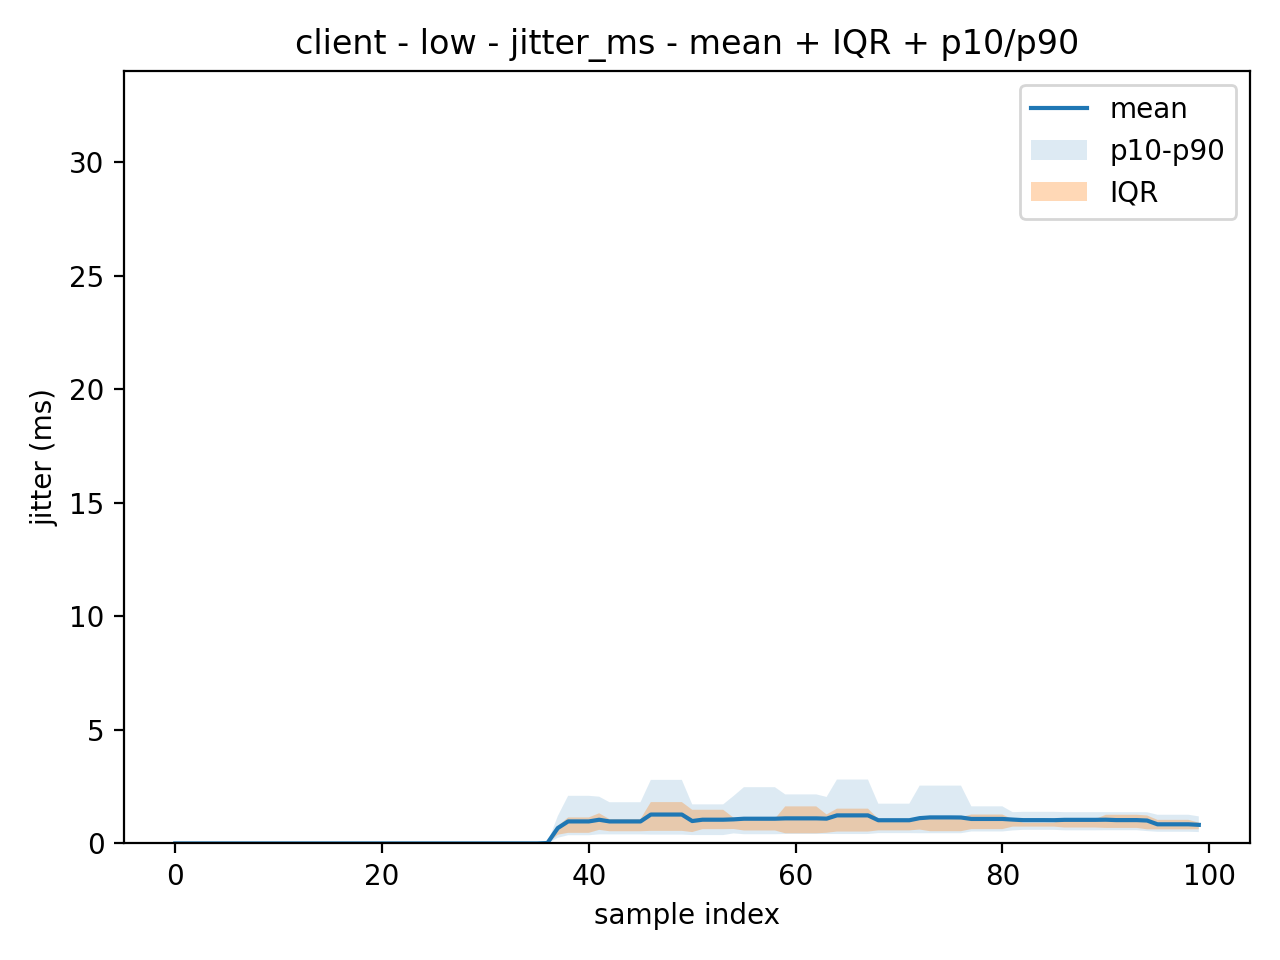
\includegraphics[width=\linewidth]{
      pars_plots/ntpsec/_aggregated/client/low/jitter_ms_mean_iqr_p10_p90.png
    }
    \caption{Scenario LOW}
  \end{subfigure}
  \hfill
  \begin{subfigure}
    {0.32\textwidth}
    \centering
    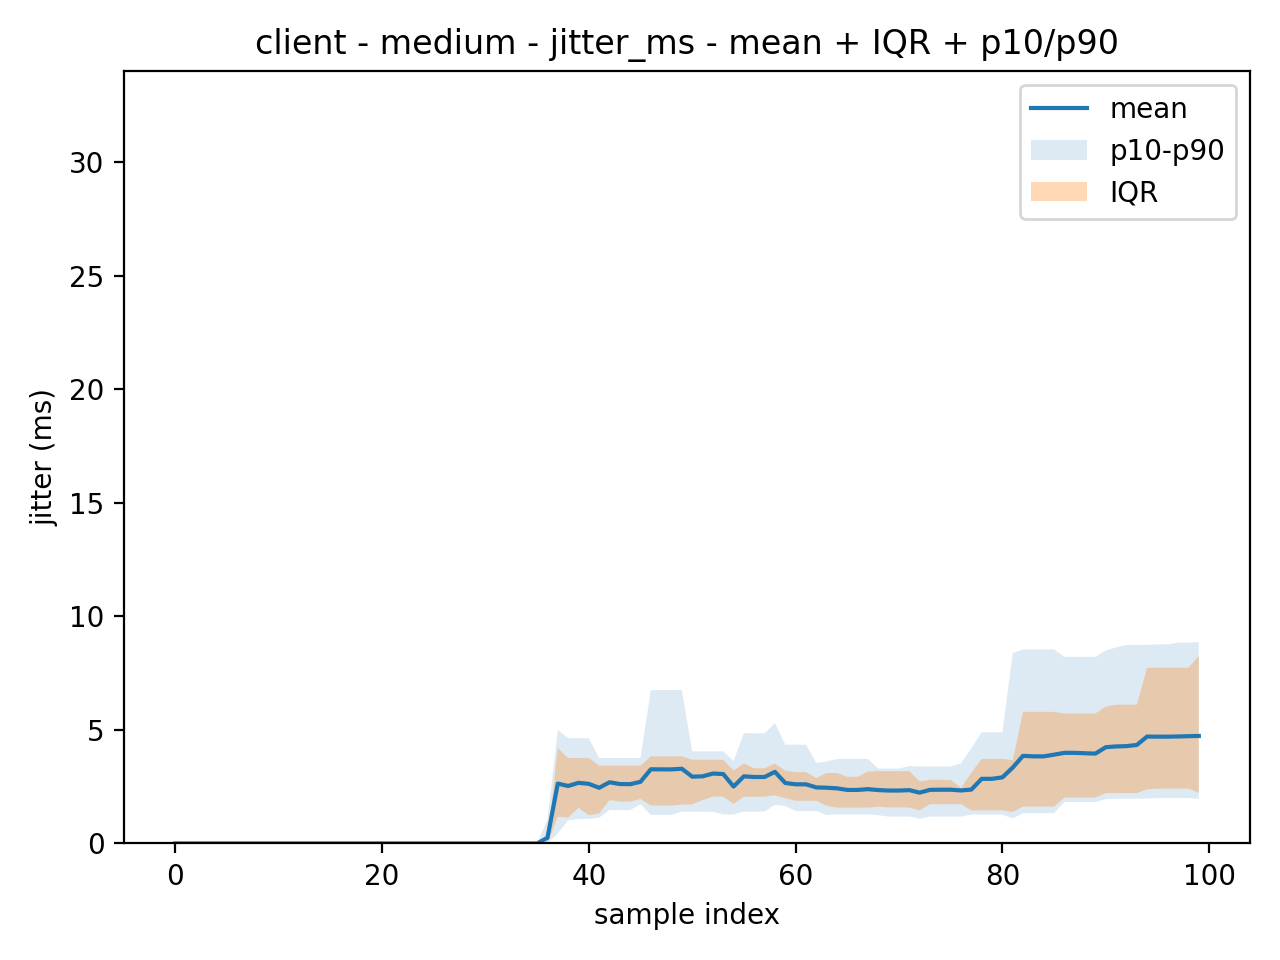
\includegraphics[width=\linewidth]{
      pars_plots/ntpsec/_aggregated/client/medium/jitter_ms_mean_iqr_p10_p90.png
    }
    \caption{Scenario MEDIUM}
  \end{subfigure}
  \hfill
  \begin{subfigure}
    {0.32\textwidth}
    \centering
    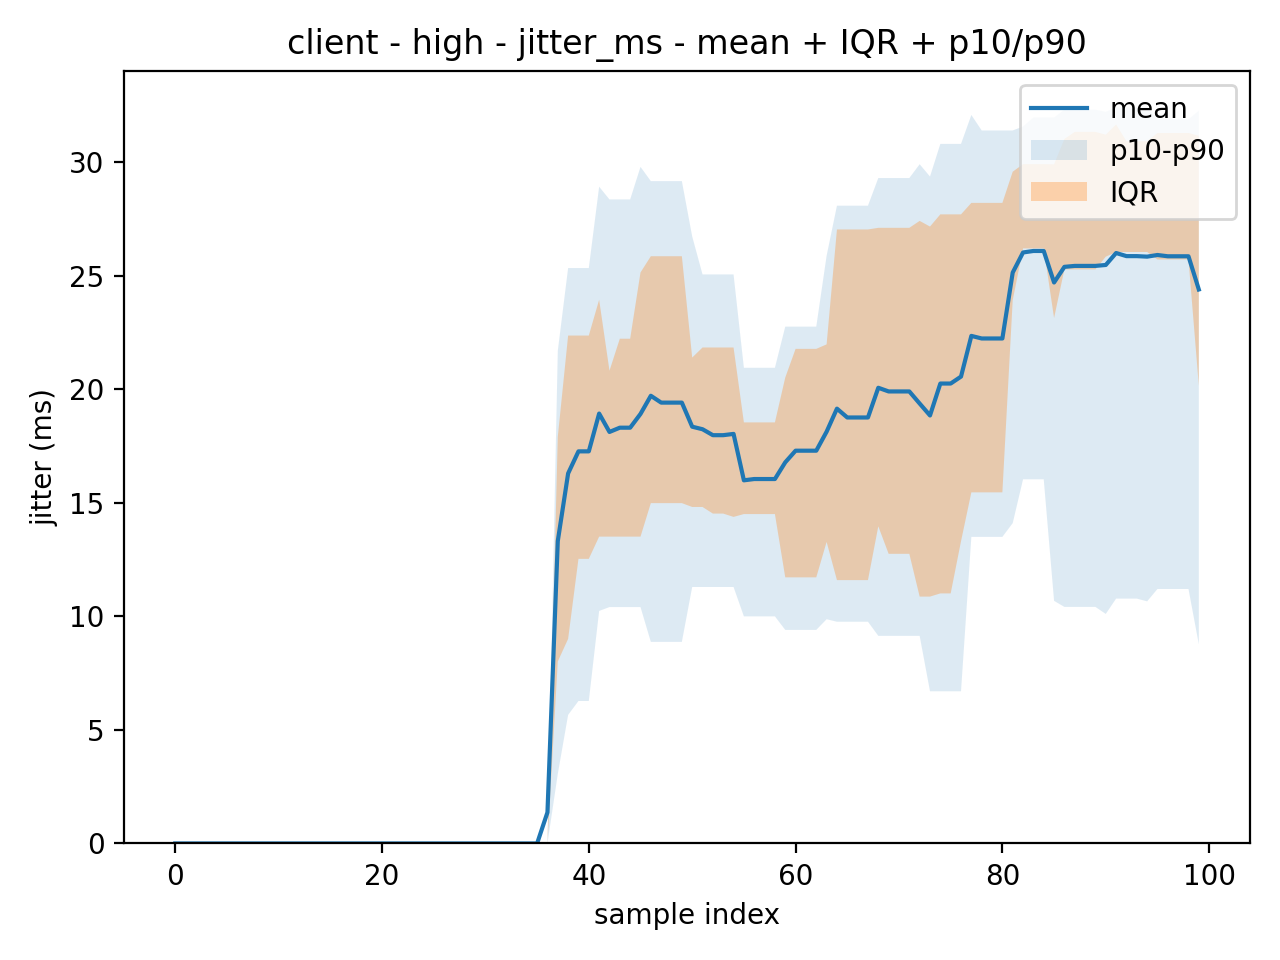
\includegraphics[width=\linewidth]{
      pars_plots/ntpsec/_aggregated/client/high/jitter_ms_mean_iqr_p10_p90.png
    }
    \caption{Scenario HIGH}
  \end{subfigure}

  \caption{Media con banda inter-quartile e banda p10-p90 - nodo: \texttt{clientntp}}
  \label{fig:scenario_comparison}
\end{figure}

L'analisi del jitter mostra un incremento di degrado attraverso un progressivo
aumento del livello medio e della variabilità.

Nello scenario \texttt{low} il valore medio risulta ~1.05 ms, con una dispersione
moderata. La banda inter-quartile media della curva aggregata è pari a ~0.65 ms,
invece la banda p10--p90 si attesta intorno a ~1.46 ms. Il comportamento osservato
è coerente con un degrado debole, evidenziando una condizione di rete stabile.

Nel caso \texttt{medium}, il jitter cresce in modo evidente e si posiziona su
una fascia sensibilmente superiore.Il valore medio è ~3.14 ms, all'incirca tre
volte il corrispondente valore osservato nello scenario \texttt{low}. Si ha un
aumento della dispersione, con banda inter-quartile media di ~2.40 ms e banda p10--p90
di ~4.18 ms.

Nello scenario \texttt{high} si manifesta un degradato più marcato. Il jitter
assume valori elevati lungo l'intera serie aggregata, con una media all'incirca di
20.9 ms. Sia ha un incremento rispetto agli scenari precedenti, in particolare rispetto
allo scenario \texttt{low}, con un divario di un ordine di grandezza. La
dispersione misurata aumenta con banda inter-quartile media ~9.38 ms e banda p10--p90
di circa 18.3 ms. Nel grafico si evidenzia una forte oscillazione, ampia e
persiste.

Vi è un generale aumento coerente con il degrado di rete, evidenziando un impatto
maggiore da gli scenari \texttt{low-medium} allo scenario \texttt{high} caratterizzato
da valori medi elevati e da una dispersione significativamente maggiore.

\subsubsection{Analisi metrica: \texttt{offset}}
\begin{figure}[H]
  \centering

  \begin{subfigure}
    {0.32\textwidth}
    \centering
    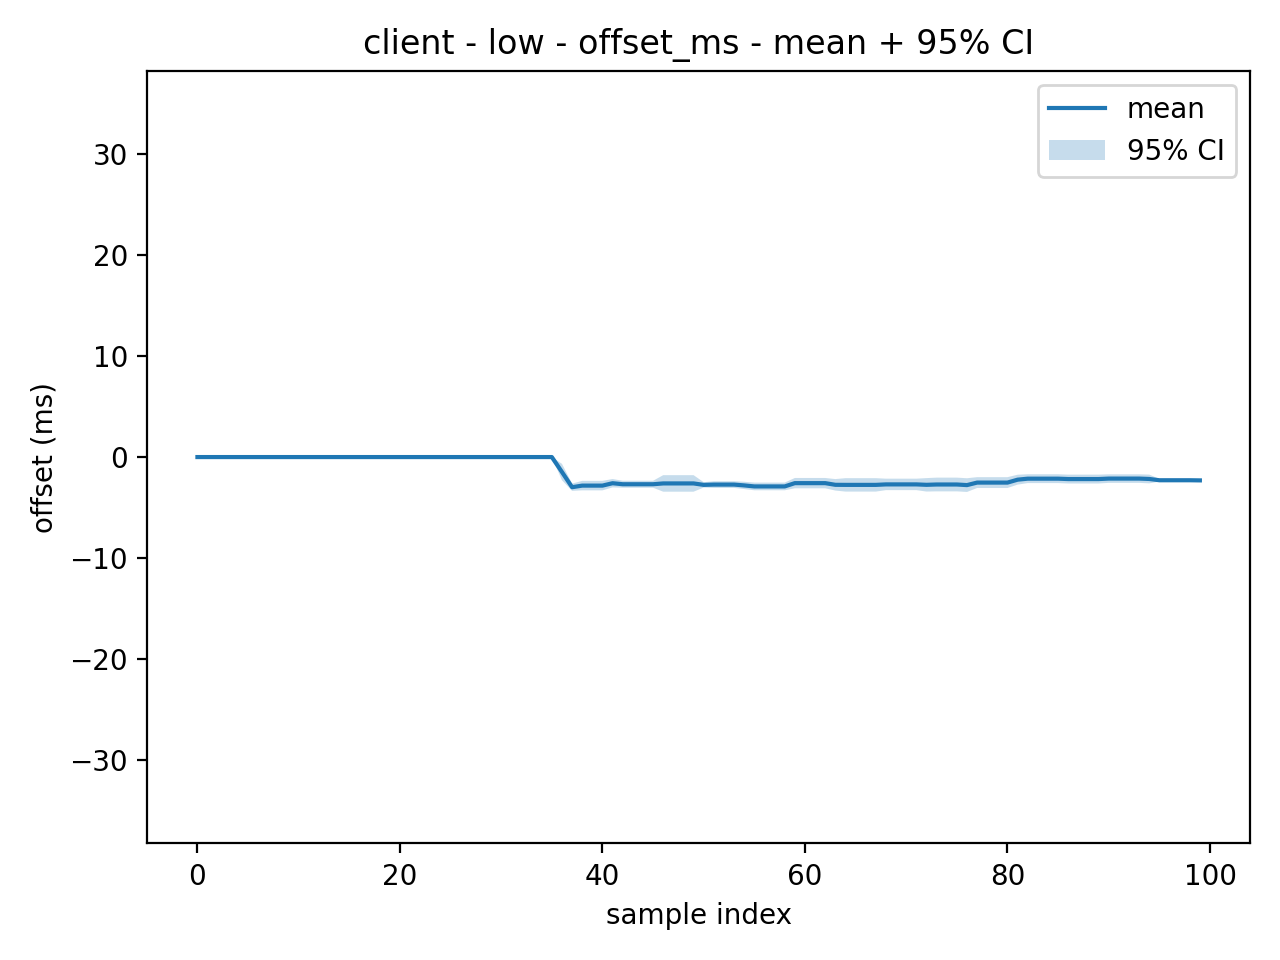
\includegraphics[width=\linewidth]{
      pars_plots/ntpsec/_aggregated/client/low/offset_ms_mean_ci95.png
    }
    \caption{Scenario LOW}
  \end{subfigure}
  \hfill
  \begin{subfigure}
    {0.32\textwidth}
    \centering
    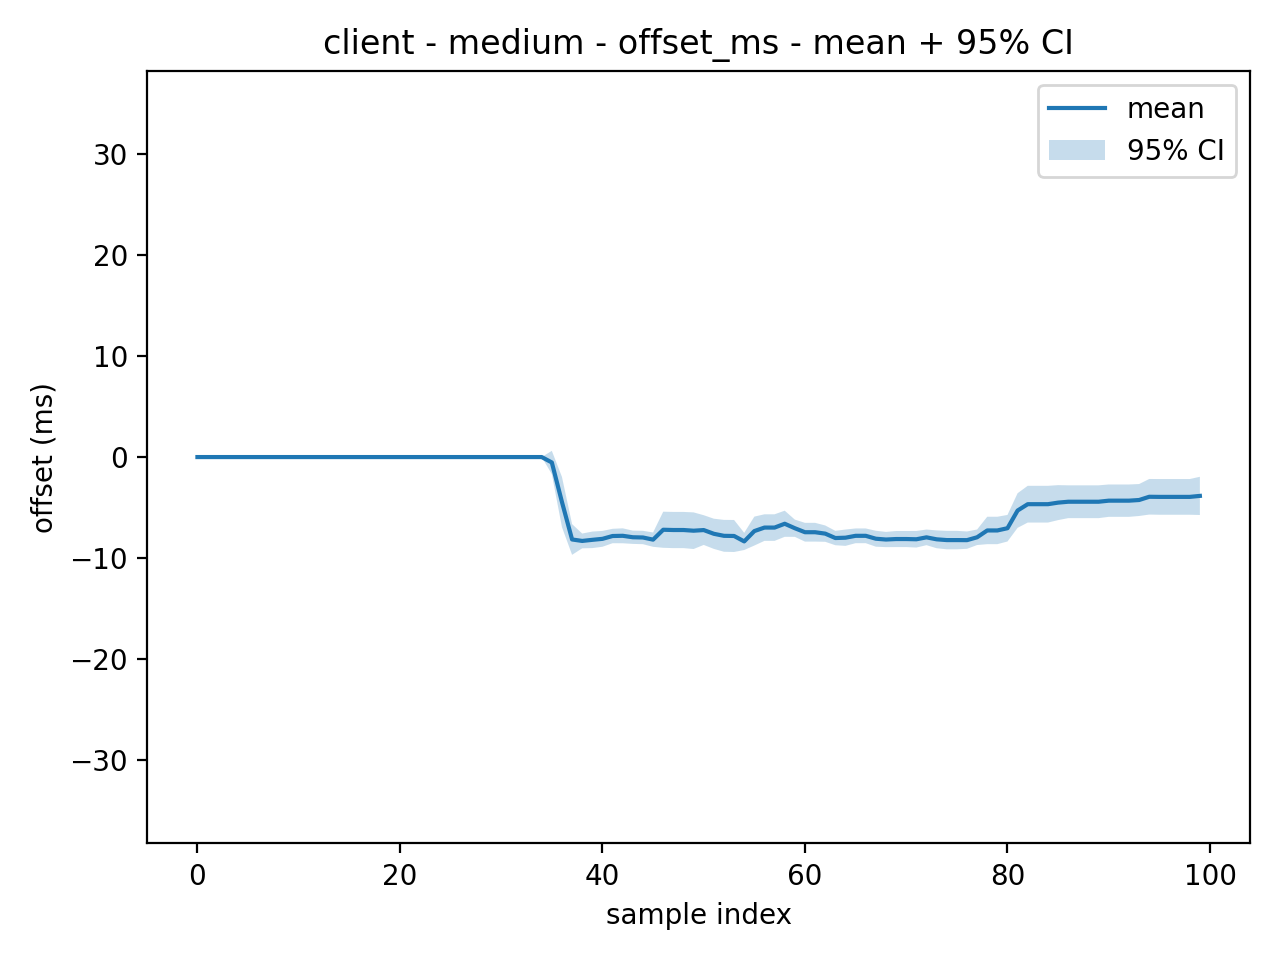
\includegraphics[width=\linewidth]{
      pars_plots/ntpsec/_aggregated/client/medium/offset_ms_mean_ci95.png
    }
    \caption{Scenario MEDIUM}
  \end{subfigure}
  \hfill
  \begin{subfigure}
    {0.32\textwidth}
    \centering
    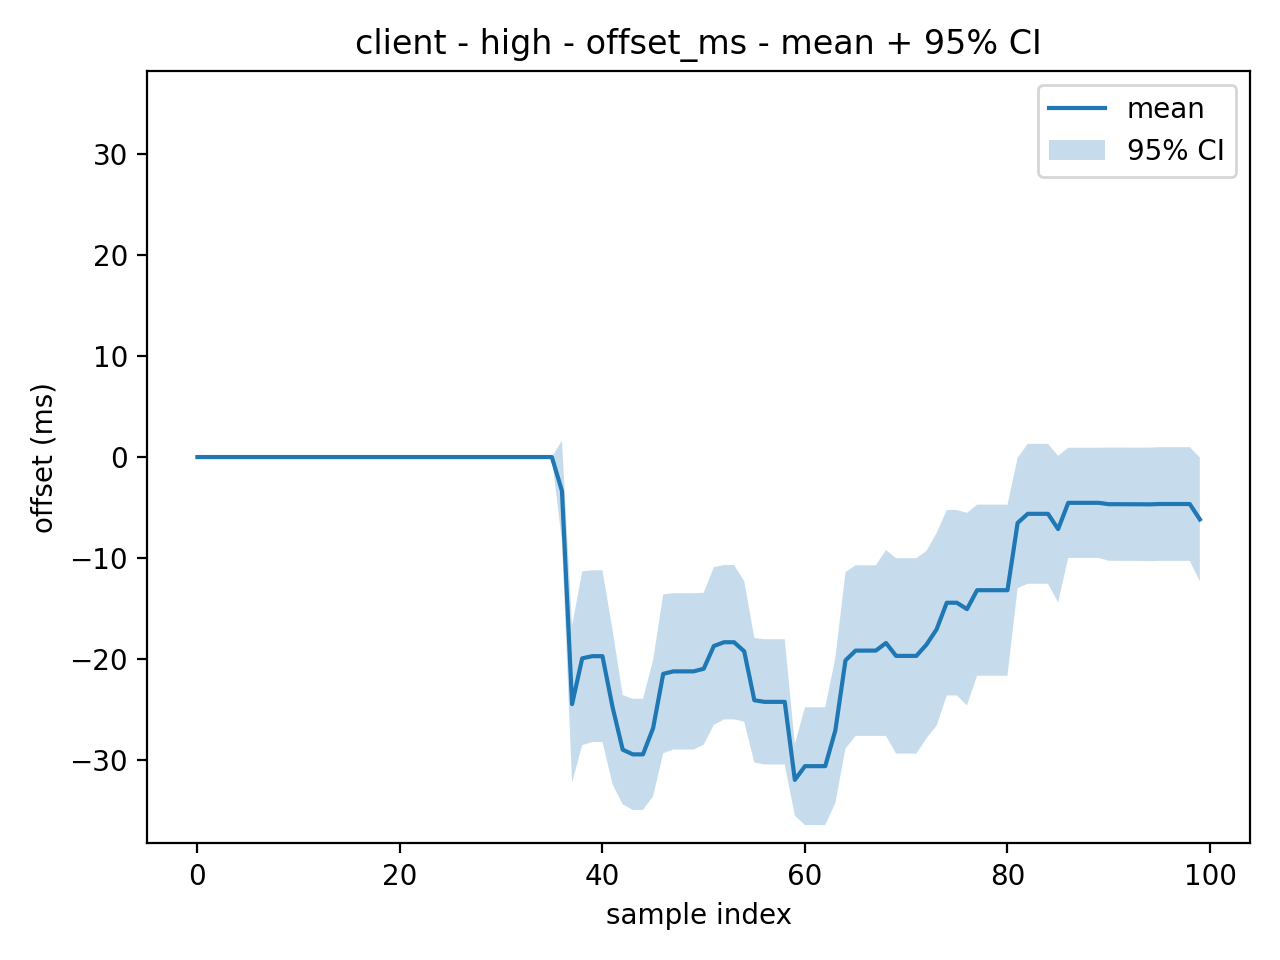
\includegraphics[width=\linewidth]{
      pars_plots/ntpsec/_aggregated/client/high/offset_ms_mean_ci95.png
    }
    \caption{Scenario HIGH}
  \end{subfigure}

  \caption{Media con intervallo di confidenza al 95\% - nodo: \texttt{clientntp}}
  \label{fig:scenario_comparison}
\end{figure}
\begin{figure}[H]
  \centering

  \begin{subfigure}
    {0.32\textwidth}
    \centering
    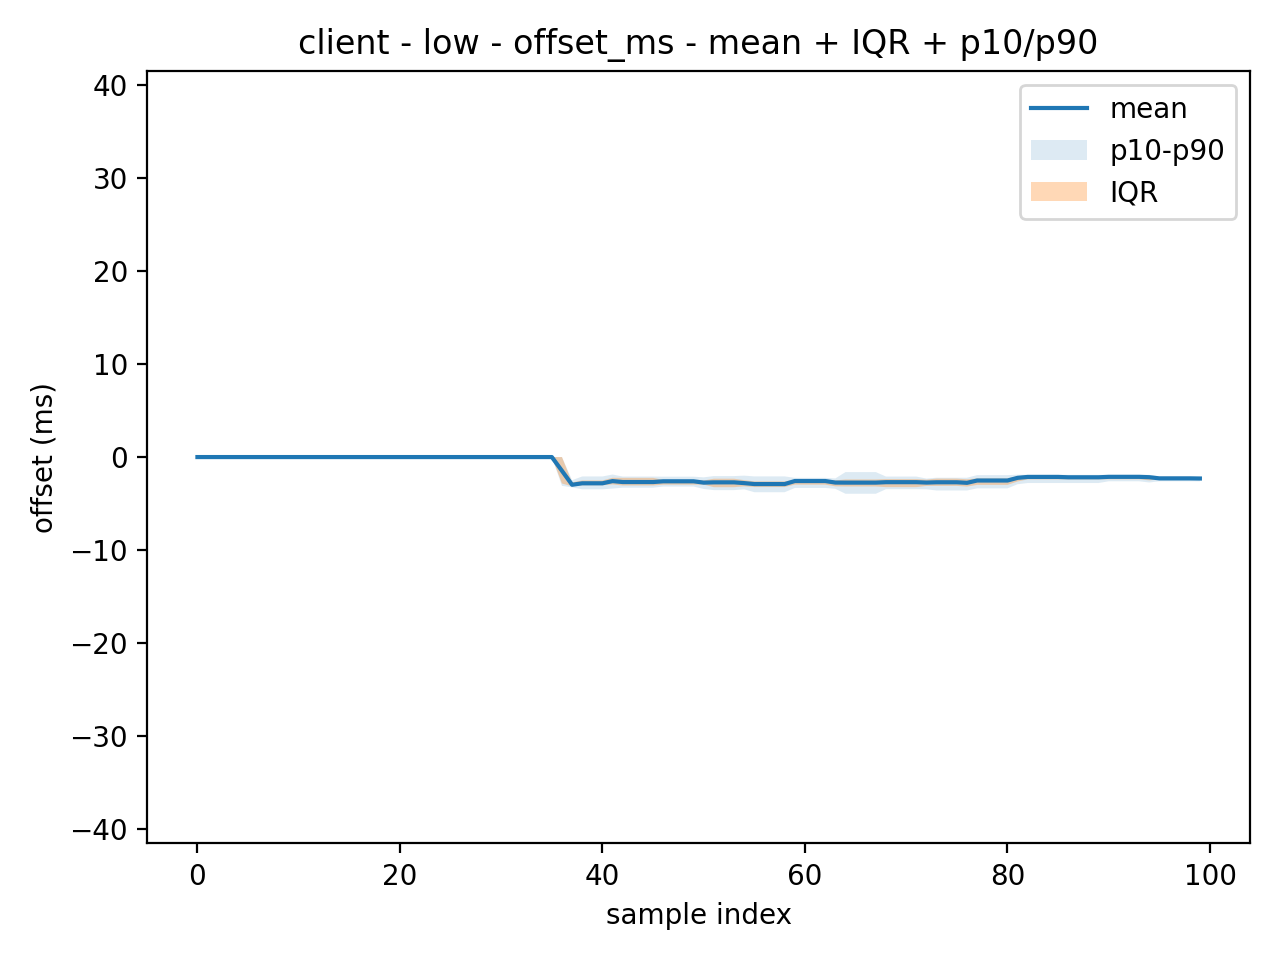
\includegraphics[width=\linewidth]{
      pars_plots/ntpsec/_aggregated/client/low/offset_ms_mean_iqr_p10_p90.png
    }
    \caption{Scenario LOW}
  \end{subfigure}
  \hfill
  \begin{subfigure}
    {0.32\textwidth}
    \centering
    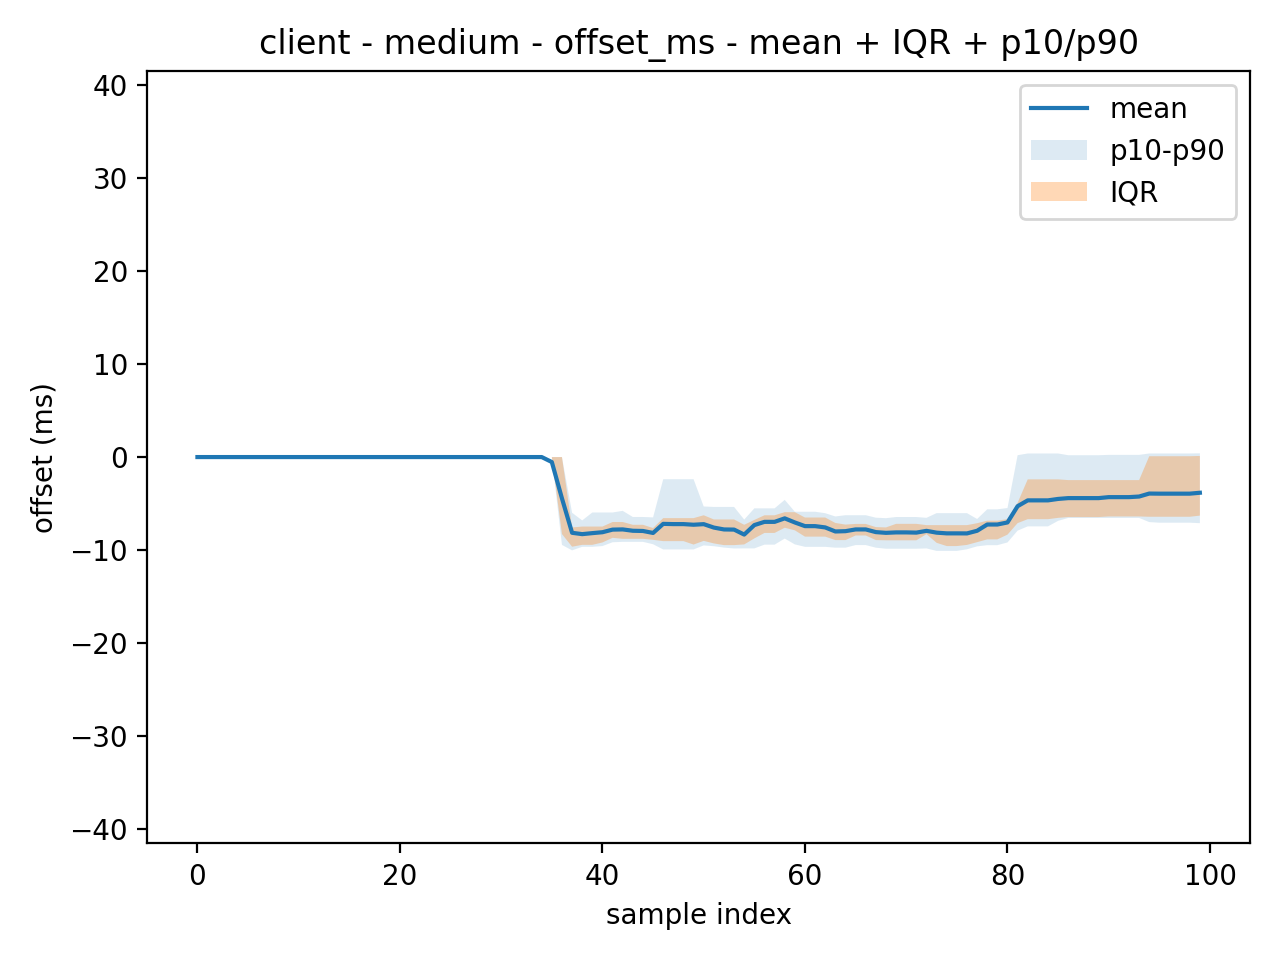
\includegraphics[width=\linewidth]{
      pars_plots/ntpsec/_aggregated/client/medium/offset_ms_mean_iqr_p10_p90.png
    }
    \caption{Scenario MEDIUM}
  \end{subfigure}
  \hfill
  \begin{subfigure}
    {0.32\textwidth}
    \centering
    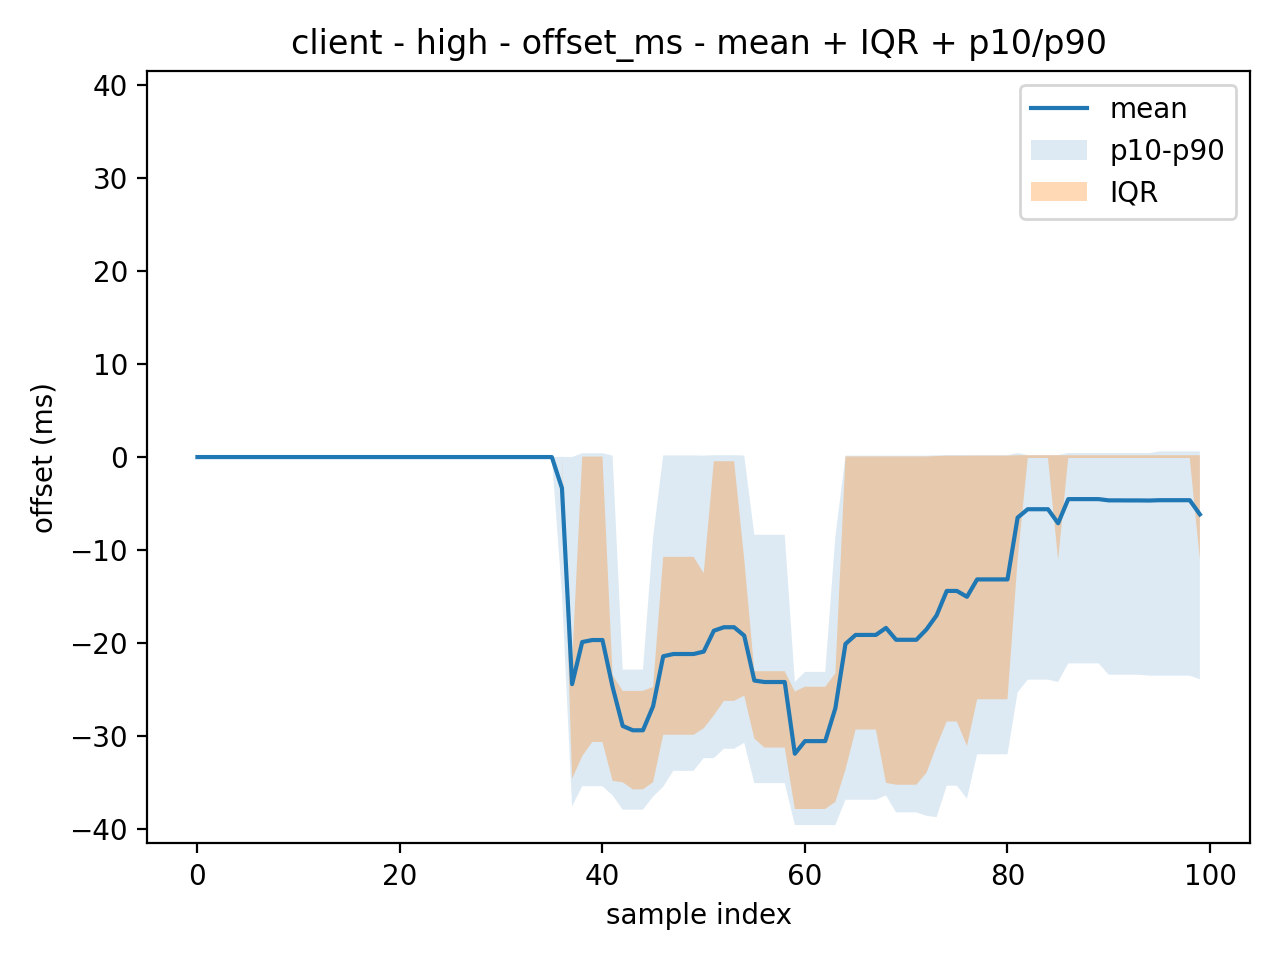
\includegraphics[width=\linewidth]{
      pars_plots/ntpsec/_aggregated/client/high/offset_ms_mean_iqr_p10_p90.png
    }
    \caption{Scenario HIGH}
  \end{subfigure}

  \caption{Media con banda inter-quartile e banda p10-p90 - nodo: \texttt{clientntp}}
  \label{fig:scenario_comparison}
\end{figure}

Nell'analisi dell'offset si evidenziano valori sistematicamente negativi.

Nello scenario \texttt{low}, l'offset si stabilizza su valori nell'intervallo ~$-
2.5$/$-3\,\mathrm{ms}$. La media è di ~$-2.55\,\mathrm{ms}$. La mediana è
pressoché identica, $-2 .55\,\mathrm{ms}$. La dispersione è moderata, ($\sigma \approx
0.91\,\mathrm{ms}$). La curva aggregata conferma il trend con un valore medio
centrale di $-2.55\,\mathrm{ms}$, invece l'ampiezza banda inter-quartile è di ~($\mathrm{IQR}
\approx 0.56\,\mathrm{ms}$) e la fascia $p10$--$p 90$ di circa ($\approx 1.21\,\mathrm{ms}$).Il
comportamento è stabile e uno scostamento limitato rispetto al riferimento.

Nel caso \texttt{medium} si ha un offset traslato su valori più marcati (negativi).
La misura è in un intervallo di $-7$/$-8\,\mathrm{ms}$, con un aumento nella
fase finale della serie. La media è ~$-6.70\,\mathrm{ms}$, con mediana pari a $-7
.08\,\mathrm{ms}$. La deviazione standard è di ~$2.81\,\mathrm{ms}$. La curva
aggregata rimane coerente con un valor medio centrale di $-6.69\,\mathrm{ms}$. C'è
una crescita anche della variabilità, mostrato dall'ampiezza media della banda
inter-quartile ($\approx 2.74\,\mathrm{ms}$) e della fascia $p10$--$p90$ ($\approx
4.97\,\mathrm{ms}$).

Lo scenario \texttt{high}, conferma il trend. La curva aggregata evidenzia una
prolungata permanenza dei valori in una fascia di circa $-20$ e
$-30\,\mathrm{ms}$ per poi avere valori che si stabiliscono nella parte finale
della run. La media pari a circa $-16.42\,\mathrm{ms}$, la mediana a
$-21.87\,\mathrm{ms}$ e la deviazione standard a circa $15.38\,\mathrm{ms}$
confermano quanto osservato. Vi è una dispersione superiore rispetto agli altri scenari.
L'ampiezza media della banda inter-quartile è di ~$15 .17\,\mathrm{ms}$, La
fascia $p10$--$p90$ di ~$29.44\, \mathrm{ms}$. Il minimo della curva media aggregata
scende inoltre fino a circa $-30.12\,\mathrm{ms}$.
Nella fase finale si osserva una presenza più marcata dagli outlier, con una curva media
esterna alla banda inter-quartile.

La misura dell'offset conferma un coerente e progressivo degrado al variare degli
impairment. Nello scenario \texttt{high} si ha un peggioramento marcato.

\subsection{\texttt{boundary}}
Nel caso del nodo \texttt{boundary} vi è necessario fare un considerazione
preliminare. A differenza di quanto osservato sul nodo \texttt{clientntp}, gli impairment
di rete introdotti mediante \texttt{tc/netem} non impattano direttamente sul
collegamento \texttt{upstream} tra il nodo \texttt{boundary} e il nodo di
riferimento ma solamente nel ramo \texttt{downstream} tra \texttt{boundary} e
\texttt{clientntp}. Di conseguenza le metriche osservate non dovrebbero, in linea
teorica, risentirne. La sezione seguente quindi, ha come scopo verificare se i
dati sono coerenti con il sistema.

L'analisi è quindi orientata principalmente a verificare la coerenza tra tale
aspettativa teorica e i dati effettivamente osservati.

È utile notare che nell'analisi il tempo di peer-selection differente rispetto a
quello osservato sul nodo \texttt{clientntp} è tenuto in considerazione.

\subsubsection{Analisi metriche: \texttt{delay, jitter, offset}}
\begin{figure}[H]
  \centering

  \begin{subfigure}
    {0.32\textwidth}
    \centering
    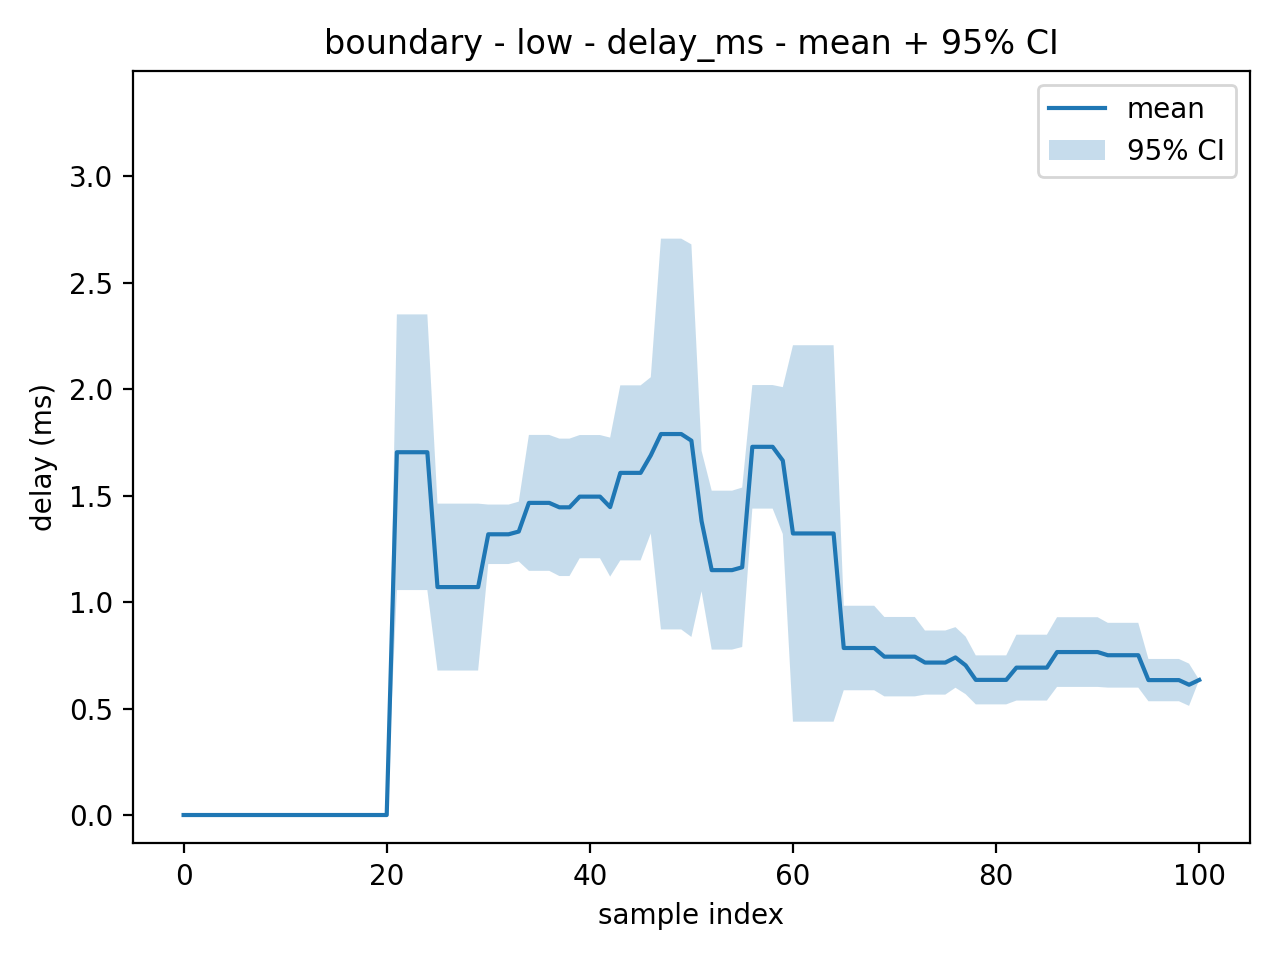
\includegraphics[width=\linewidth]{
      pars_plots/ntpsec/_aggregated/boundary/low/delay_ms_mean_ci95.png
    }
    \caption{Scenario LOW}
  \end{subfigure}
  \hfill
  \begin{subfigure}
    {0.32\textwidth}
    \centering
    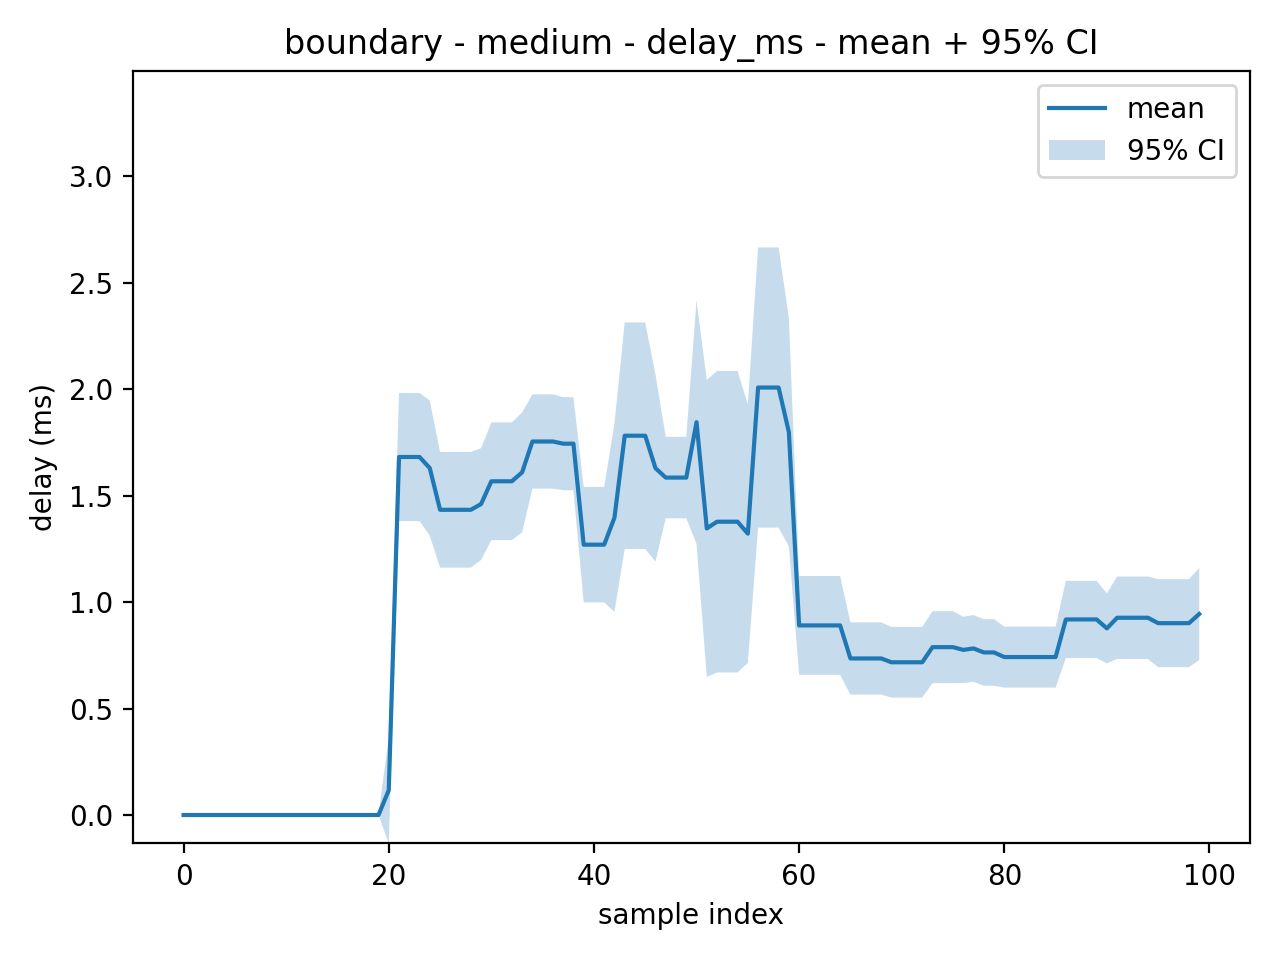
\includegraphics[width=\linewidth]{
      pars_plots/ntpsec/_aggregated/boundary/medium/delay_ms_mean_ci95.png
    }
    \caption{Scenario MEDIUM}
  \end{subfigure}
  \hfill
  \begin{subfigure}
    {0.32\textwidth}
    \centering
    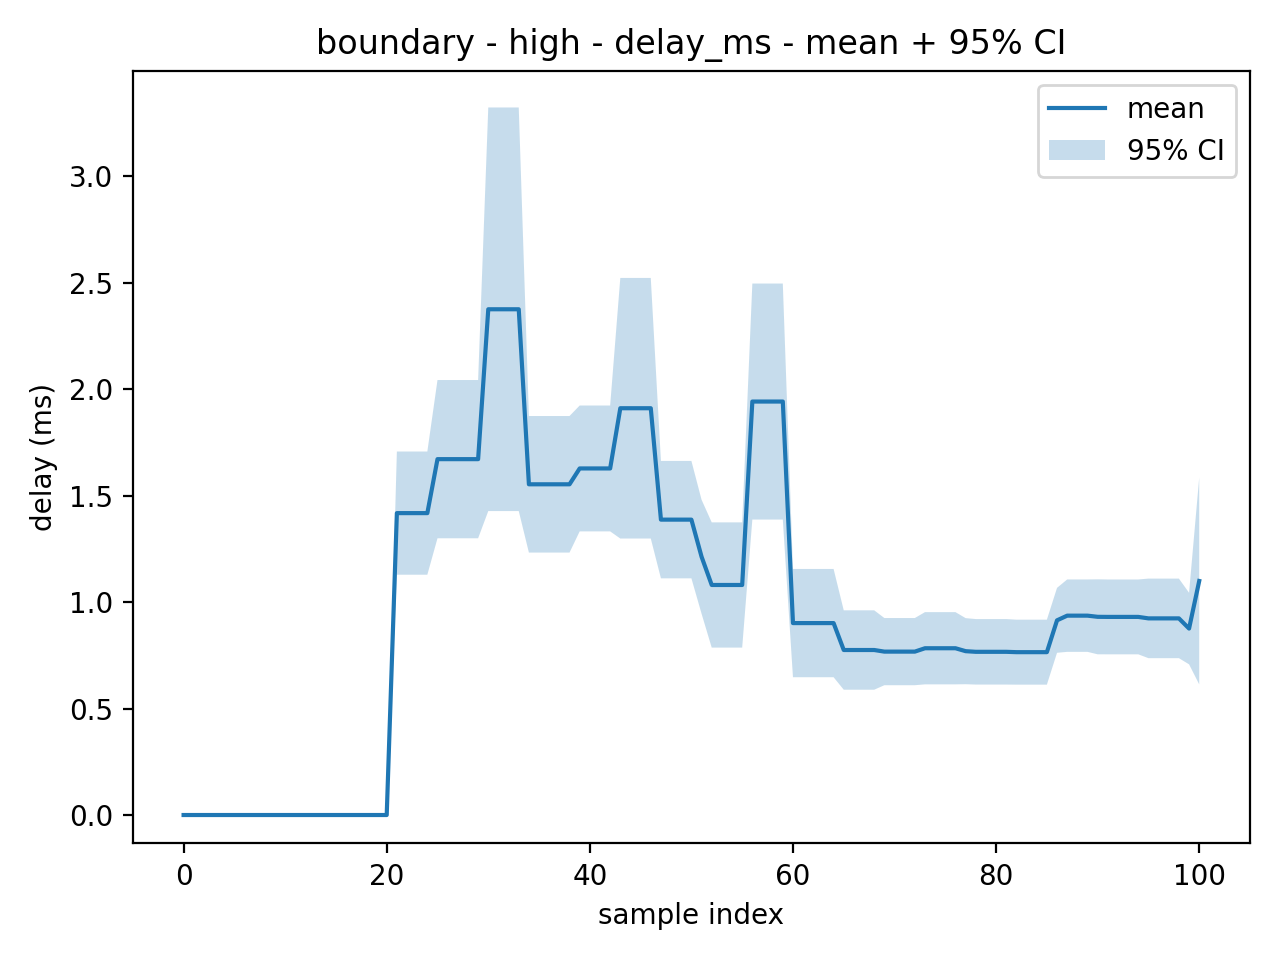
\includegraphics[width=\linewidth]{
      pars_plots/ntpsec/_aggregated/boundary/high/delay_ms_mean_ci95.png
    }
    \caption{Scenario HIGH}
  \end{subfigure}

  \caption{Media con intervallo di confidenza al 95\% - nodo: \texttt{boundary} metrica:
  \texttt{delay}}
  \label{fig:scenario_comparison}
\end{figure}
\begin{figure}[H]
  \centering

  \begin{subfigure}
    {0.32\textwidth}
    \centering
    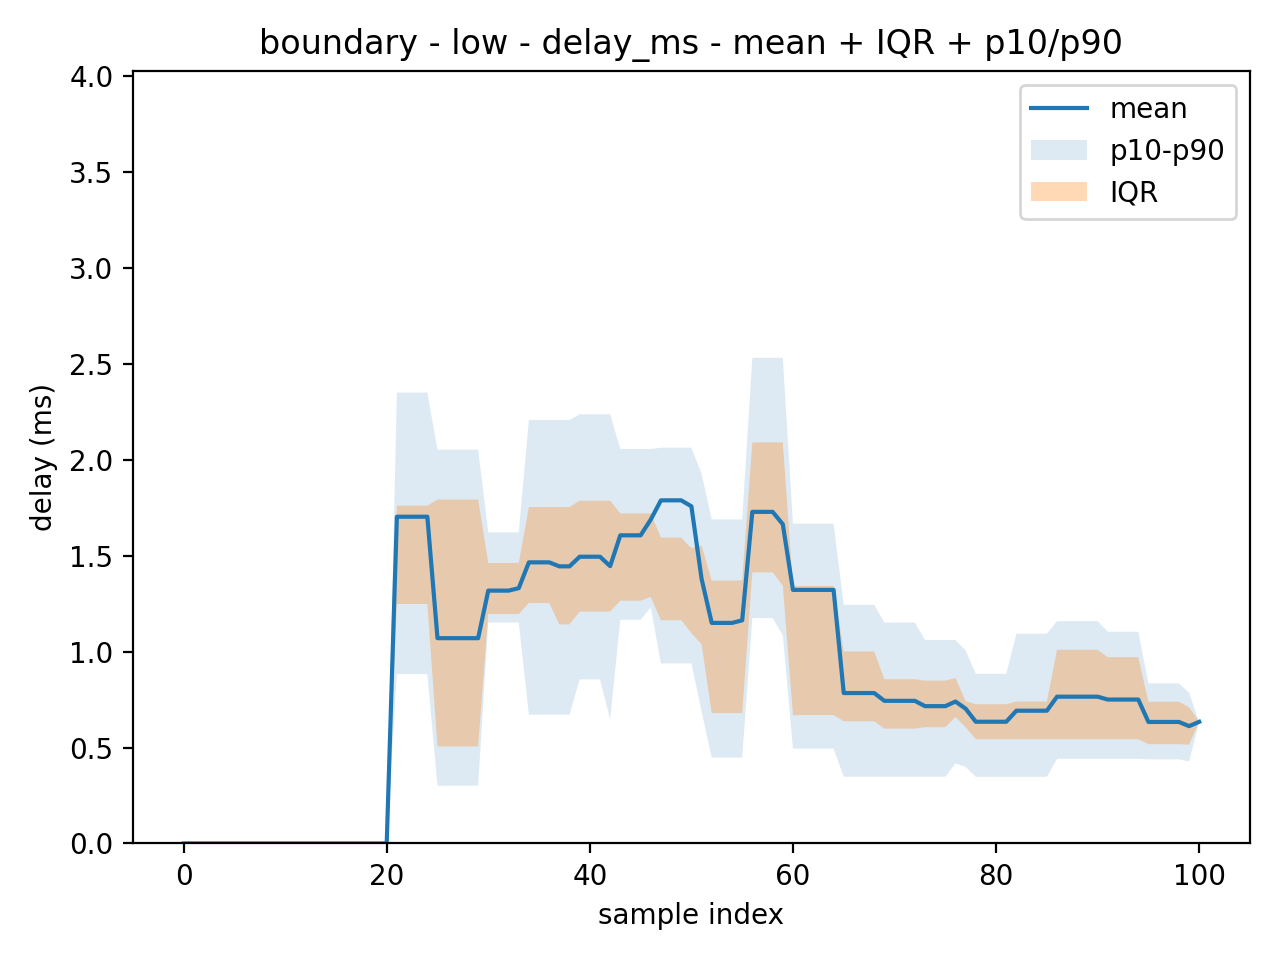
\includegraphics[width=\linewidth]{
      pars_plots/ntpsec/_aggregated/boundary/low/delay_ms_mean_iqr_p10_p90.png
    }
    \caption{Scenario LOW}
  \end{subfigure}
  \hfill
  \begin{subfigure}
    {0.32\textwidth}
    \centering
    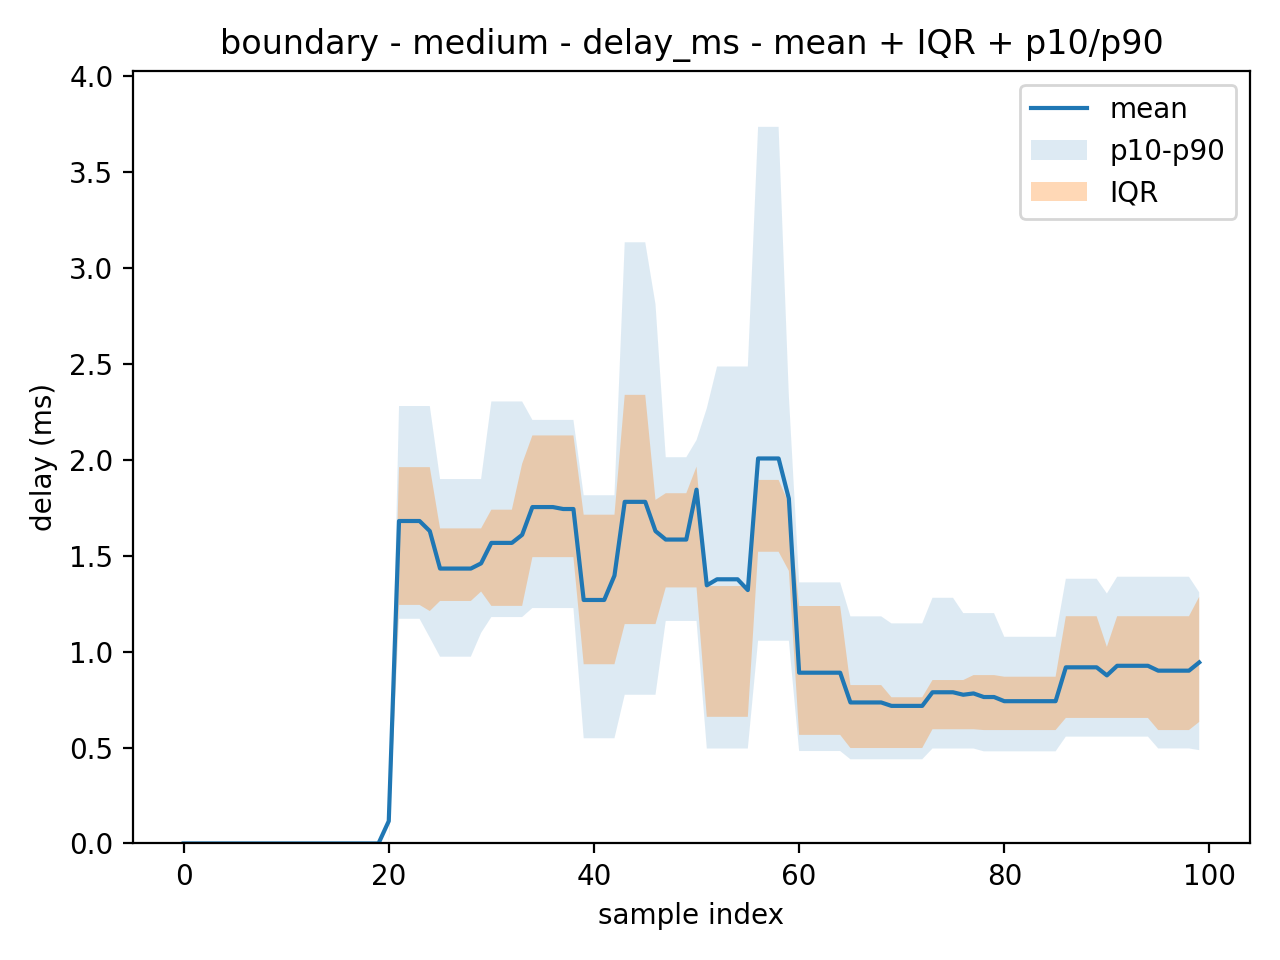
\includegraphics[width=\linewidth]{
      pars_plots/ntpsec/_aggregated/boundary/medium/delay_ms_mean_iqr_p10_p90.png
    }
    \caption{Scenario MEDIUM}
  \end{subfigure}
  \hfill
  \begin{subfigure}
    {0.32\textwidth}
    \centering
    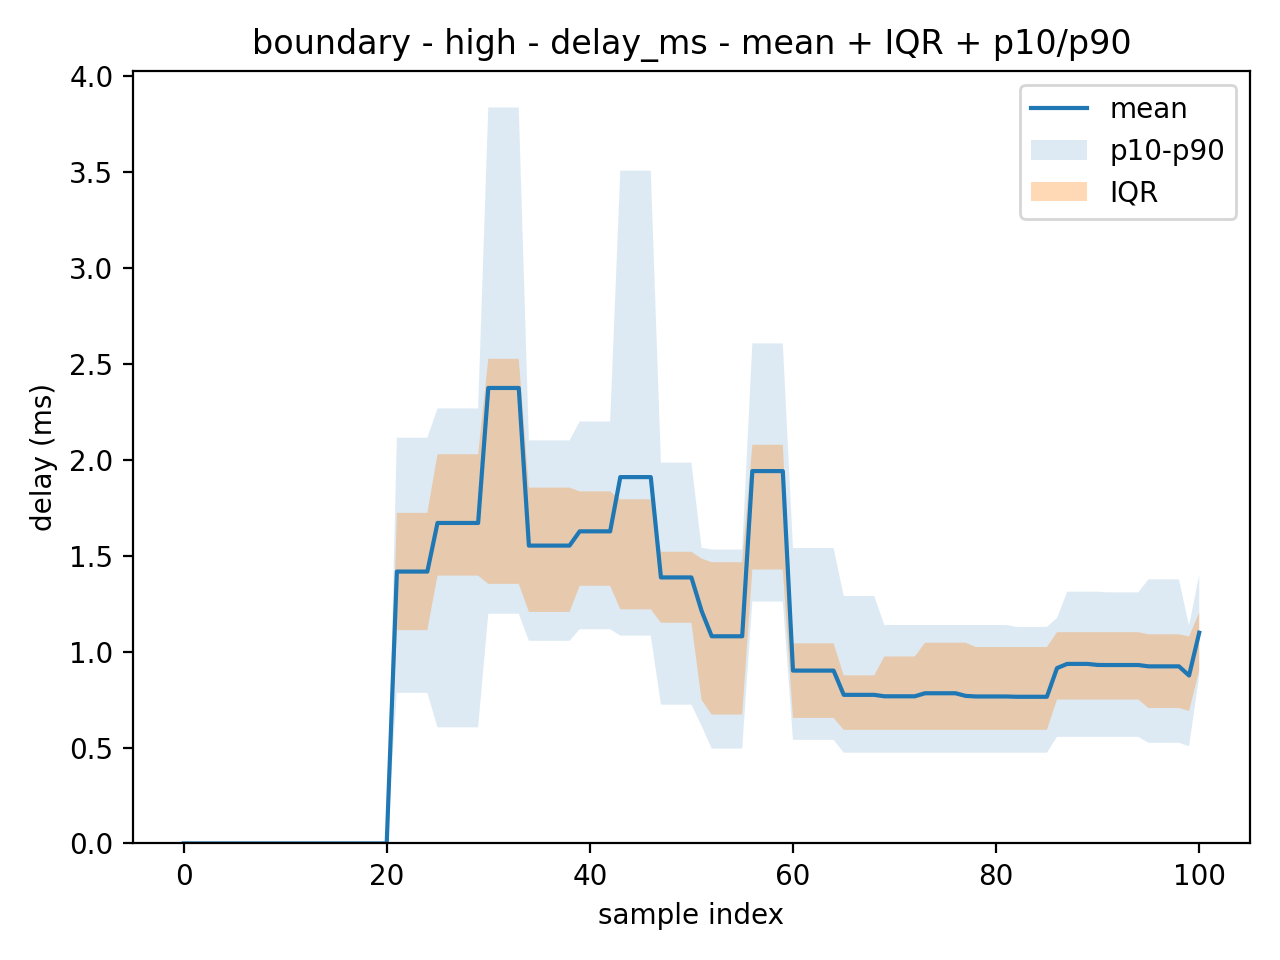
\includegraphics[width=\linewidth]{
      pars_plots/ntpsec/_aggregated/boundary/high/delay_ms_mean_iqr_p10_p90.png
    }
    \caption{Scenario HIGH}
  \end{subfigure}

  \caption{Media con banda inter-quartile e banda p10-p90 - nodo: \texttt{boundary}
  metrica: \texttt{delay}}
  \label{fig:scenario_comparison}
\end{figure}

\hrule

\begin{figure}[H]
  \centering

  \begin{subfigure}
    {0.32\textwidth}
    \centering
    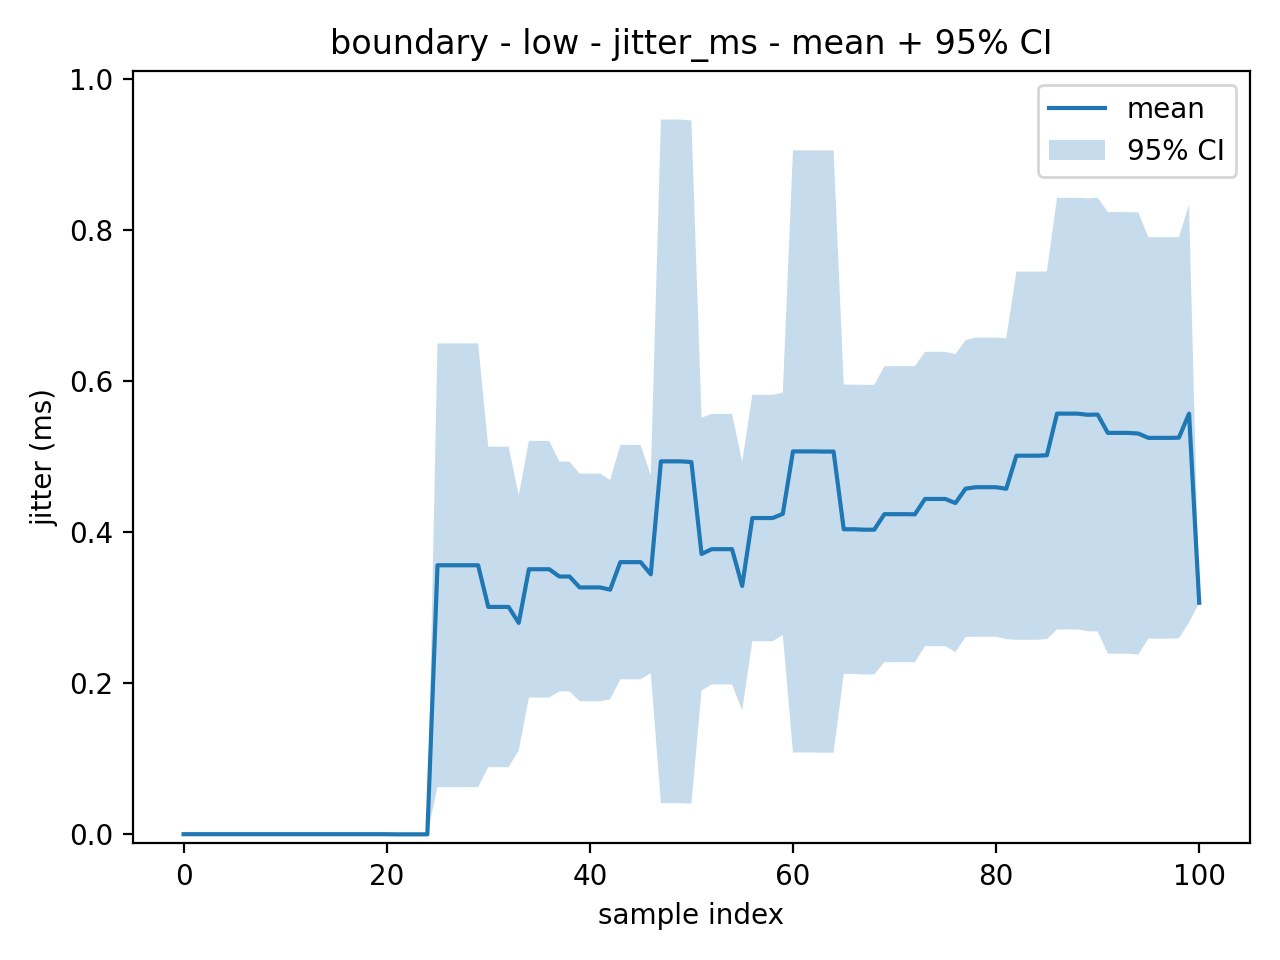
\includegraphics[width=\linewidth]{
      pars_plots/ntpsec/_aggregated/boundary/low/jitter_ms_mean_ci95.png
    }
    \caption{Scenario LOW}
  \end{subfigure}
  \hfill
  \begin{subfigure}
    {0.32\textwidth}
    \centering
    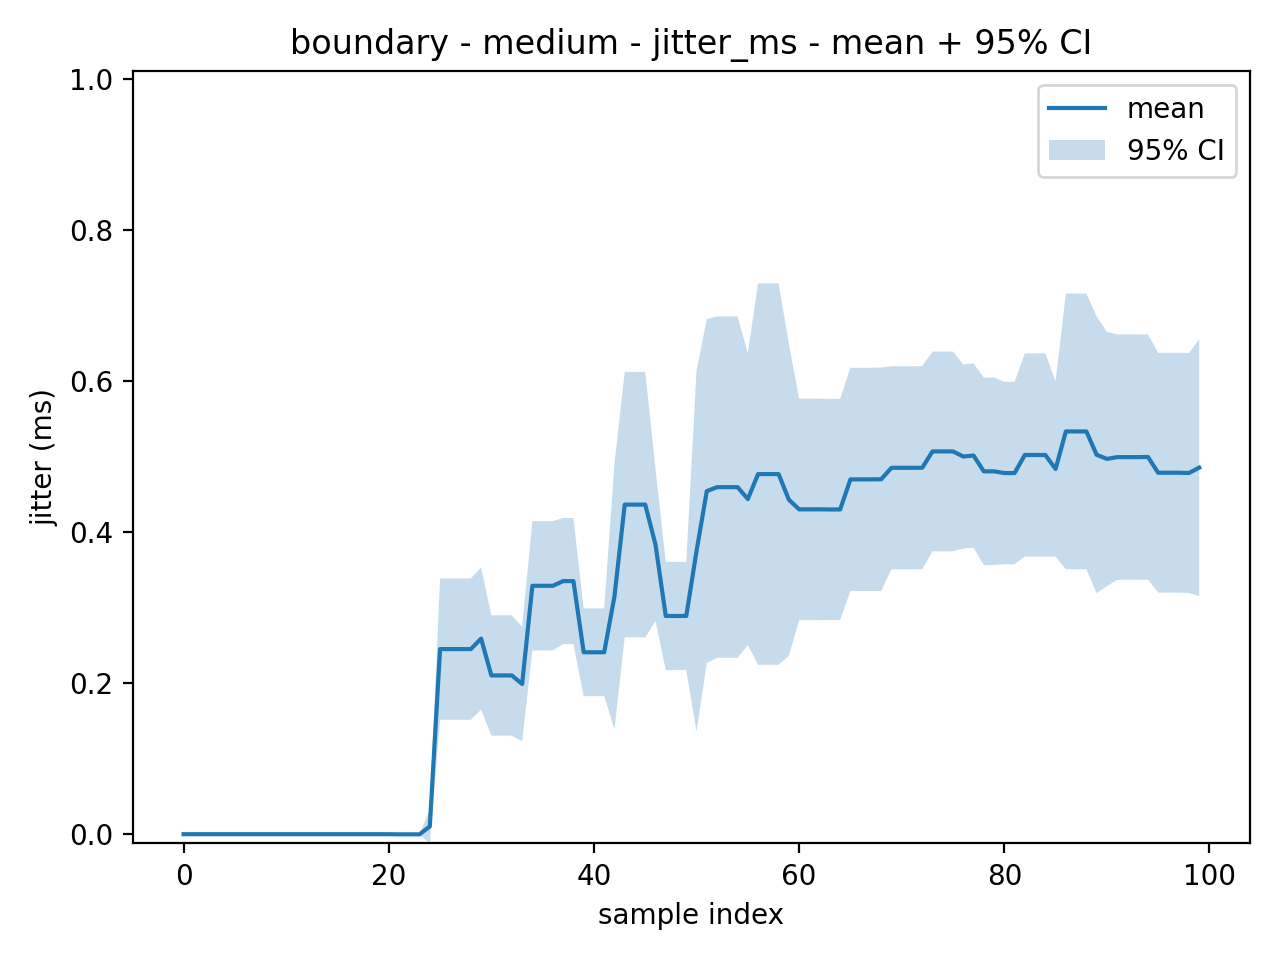
\includegraphics[width=\linewidth]{
      pars_plots/ntpsec/_aggregated/boundary/medium/jitter_ms_mean_ci95.png
    }
    \caption{Scenario MEDIUM}
  \end{subfigure}
  \hfill
  \begin{subfigure}
    {0.32\textwidth}
    \centering
    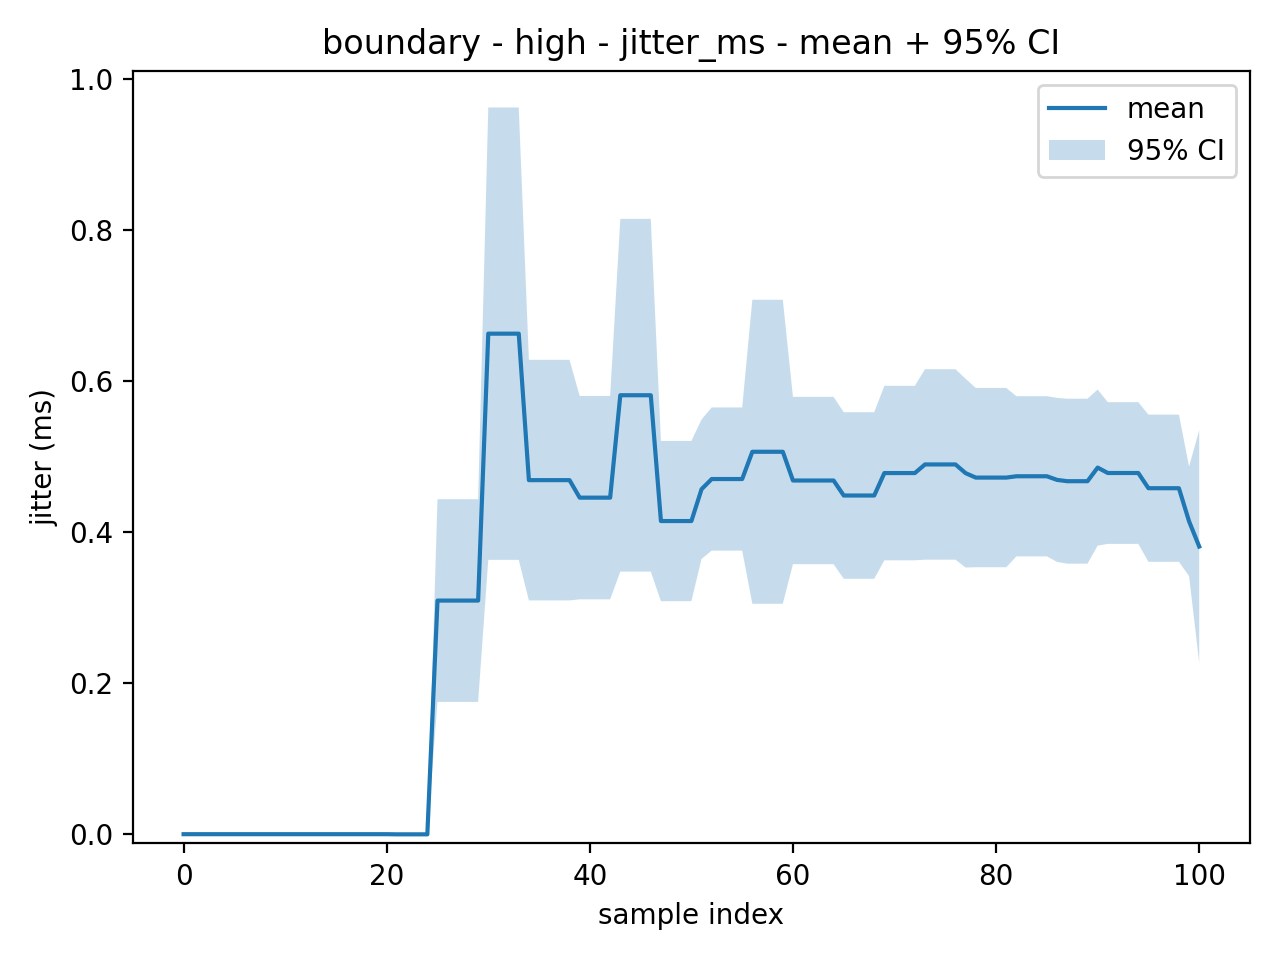
\includegraphics[width=\linewidth]{
      pars_plots/ntpsec/_aggregated/boundary/high/jitter_ms_mean_ci95.png
    }
    \caption{Scenario HIGH}
  \end{subfigure}

  \caption{Media con intervallo di confidenza al 95\% - nodo: \texttt{boundary} metrica:
  \texttt{jitter}}
  \label{fig:scenario_comparison}
\end{figure}
\begin{figure}[H]
  \centering

  \begin{subfigure}
    {0.32\textwidth}
    \centering
    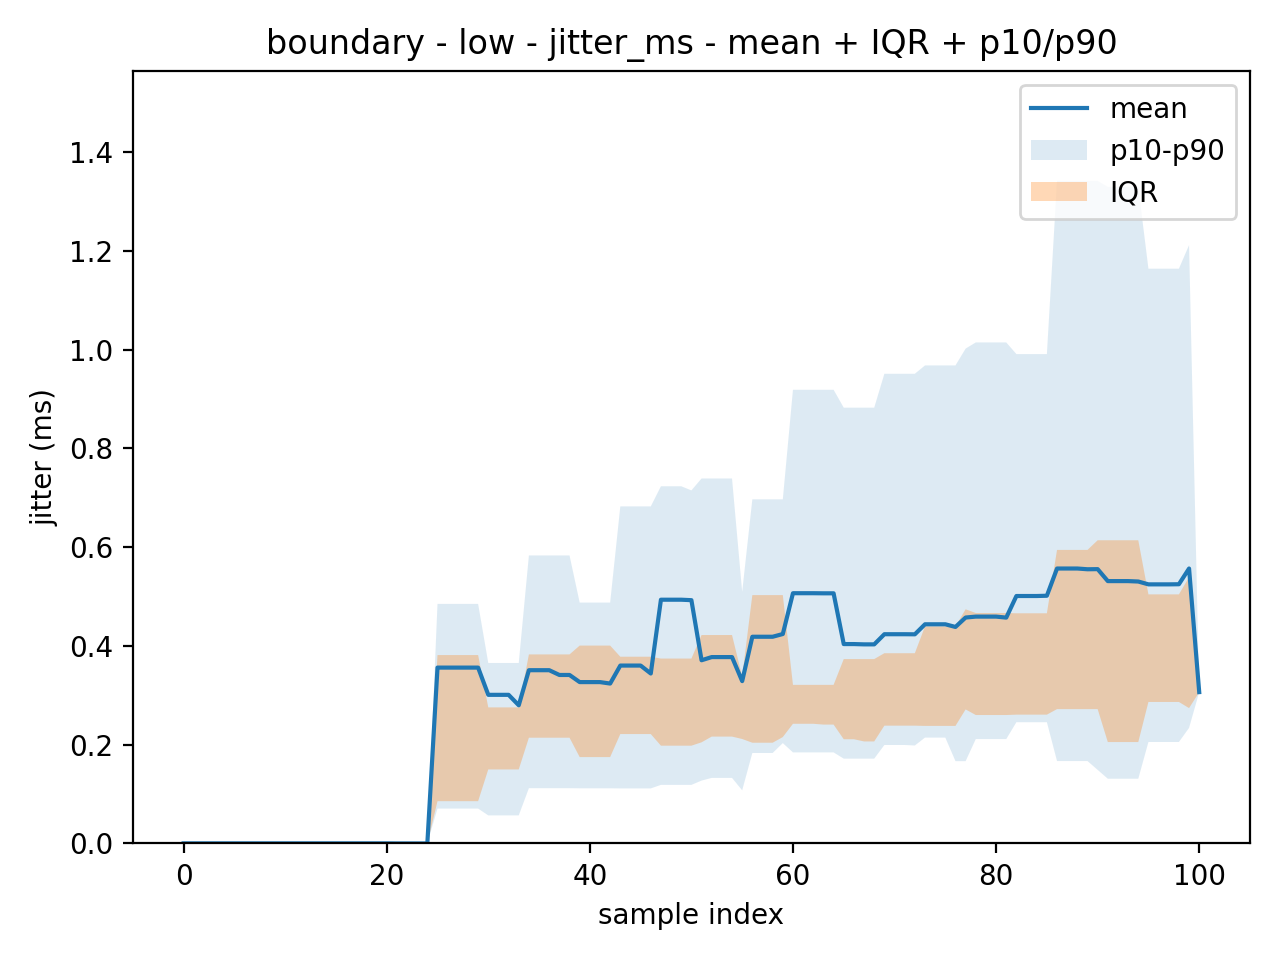
\includegraphics[width=\linewidth]{
      pars_plots/ntpsec/_aggregated/boundary/low/jitter_ms_mean_iqr_p10_p90.png
    }
    \caption{Scenario LOW}
  \end{subfigure}
  \hfill
  \begin{subfigure}
    {0.32\textwidth}
    \centering
    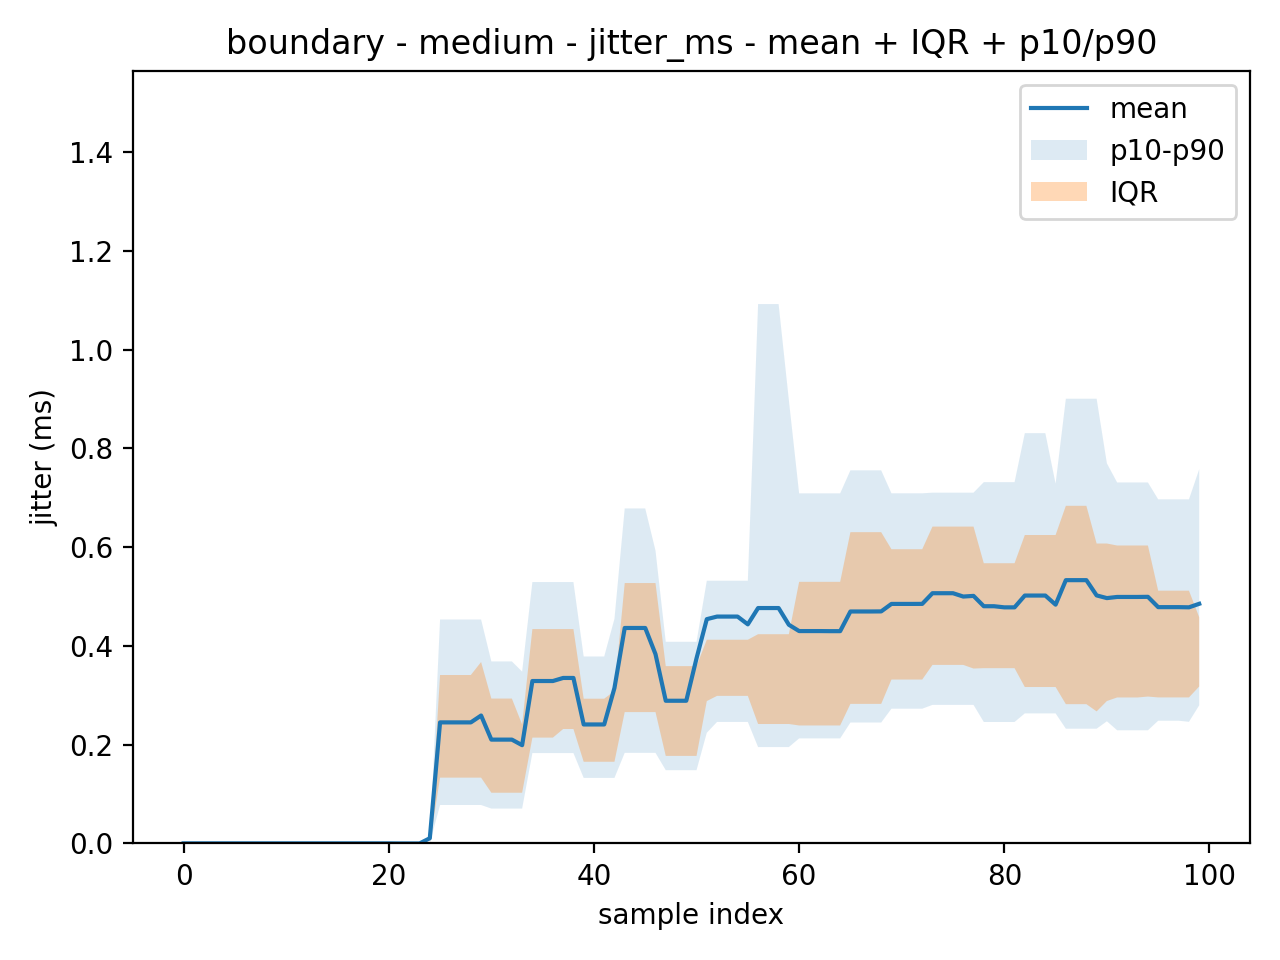
\includegraphics[width=\linewidth]{
      pars_plots/ntpsec/_aggregated/boundary/medium/jitter_ms_mean_iqr_p10_p90.png
    }
    \caption{Scenario MEDIUM}
  \end{subfigure}
  \hfill
  \begin{subfigure}
    {0.32\textwidth}
    \centering
    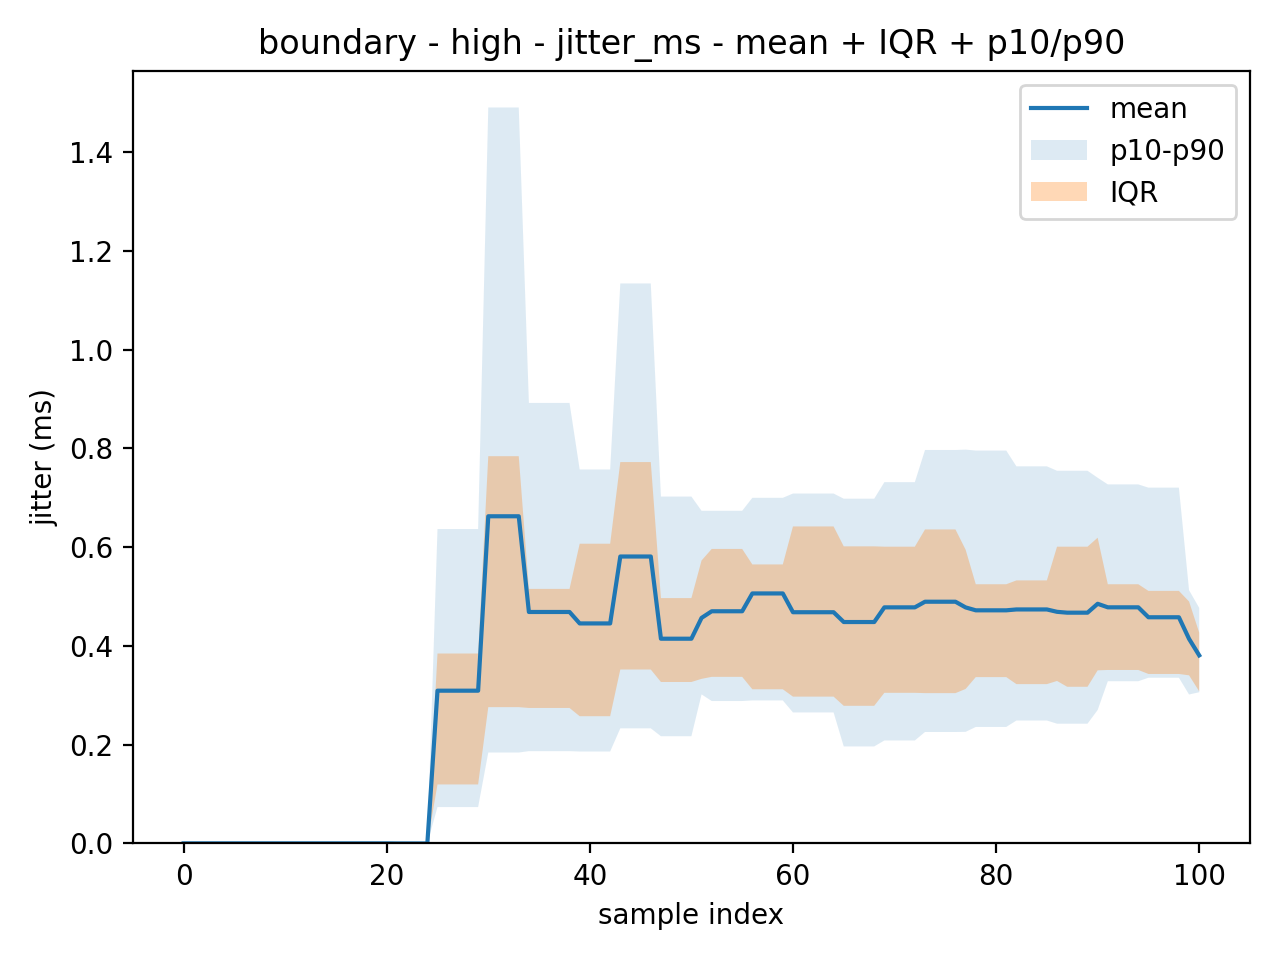
\includegraphics[width=\linewidth]{
      pars_plots/ntpsec/_aggregated/boundary/high/jitter_ms_mean_iqr_p10_p90.png
    }
    \caption{Scenario HIGH}
  \end{subfigure}

  \caption{Media con banda inter-quartile e banda p10-p90 - nodo: \texttt{boundary}
  metrica: \texttt{jitter}}
  \label{fig:scenario_comparison}
\end{figure}

\hrule

\begin{figure}[H]
  \centering

  \begin{subfigure}
    {0.32\textwidth}
    \centering
    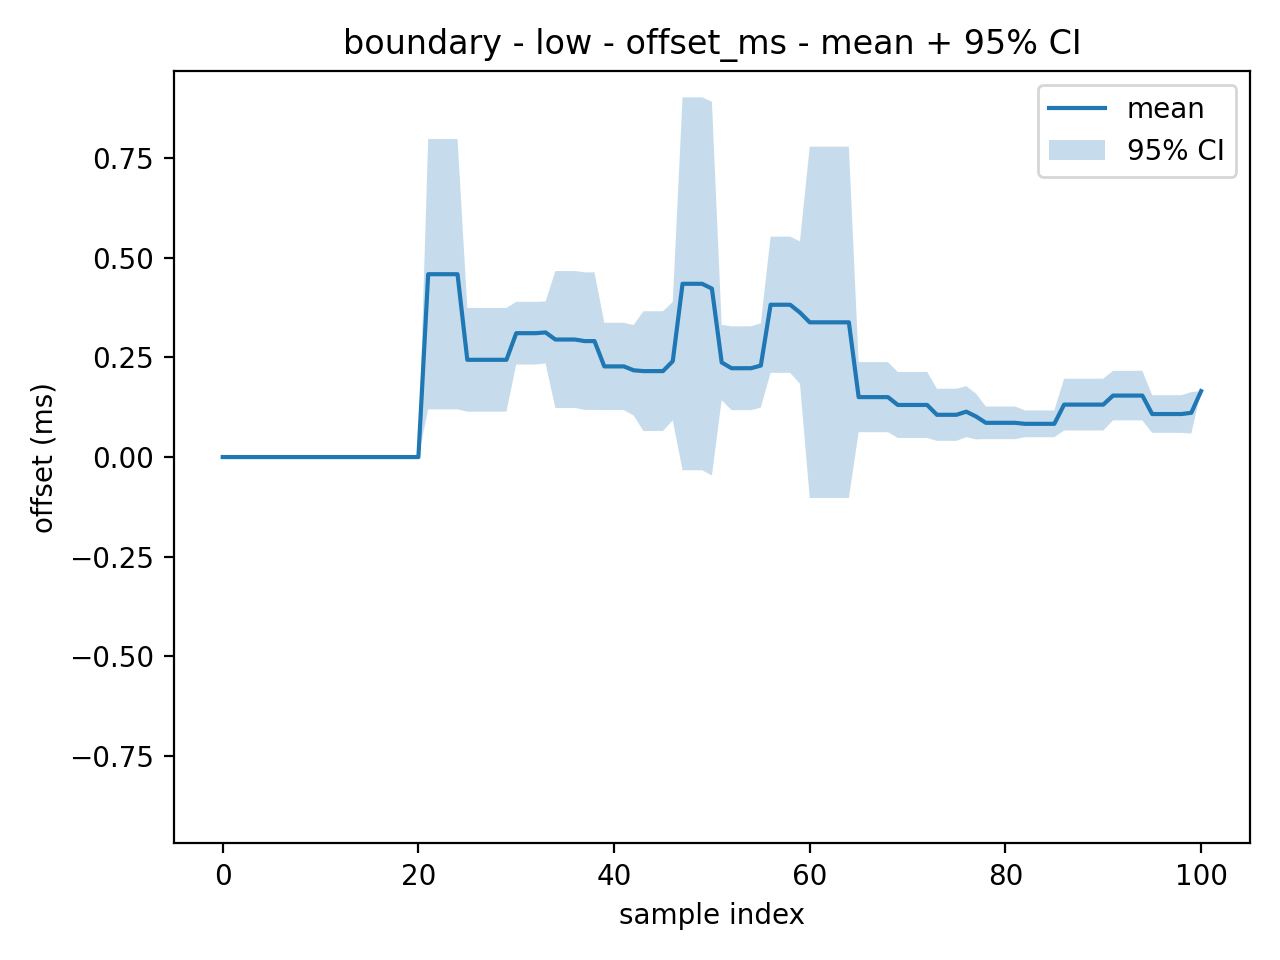
\includegraphics[width=\linewidth]{
      pars_plots/ntpsec/_aggregated/boundary/low/offset_ms_mean_ci95.png
    }
    \caption{Scenario LOW}
  \end{subfigure}
  \hfill
  \begin{subfigure}
    {0.32\textwidth}
    \centering
    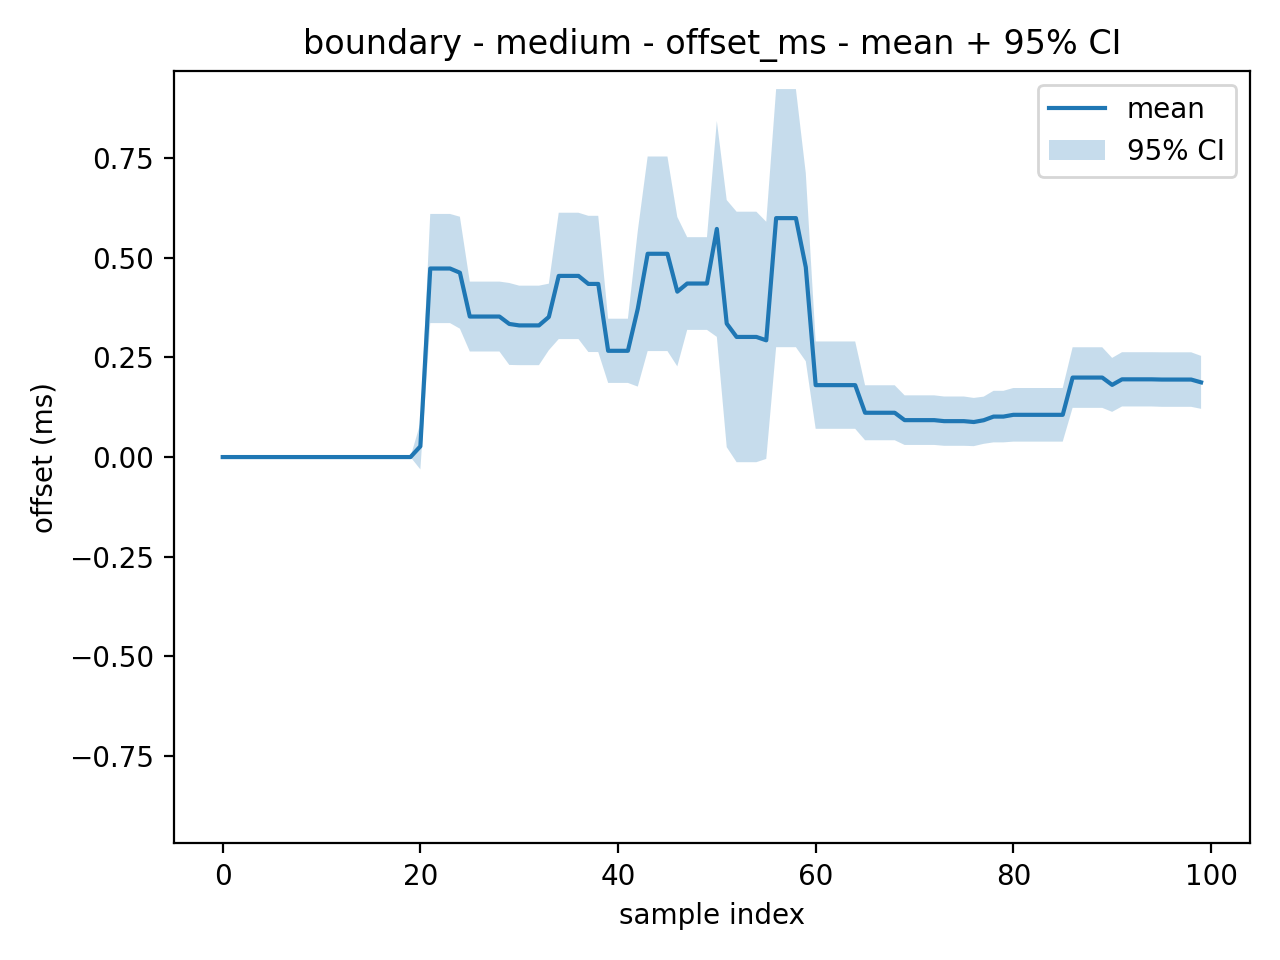
\includegraphics[width=\linewidth]{
      pars_plots/ntpsec/_aggregated/boundary/medium/offset_ms_mean_ci95.png
    }
    \caption{Scenario MEDIUM}
  \end{subfigure}
  \hfill
  \begin{subfigure}
    {0.32\textwidth}
    \centering
    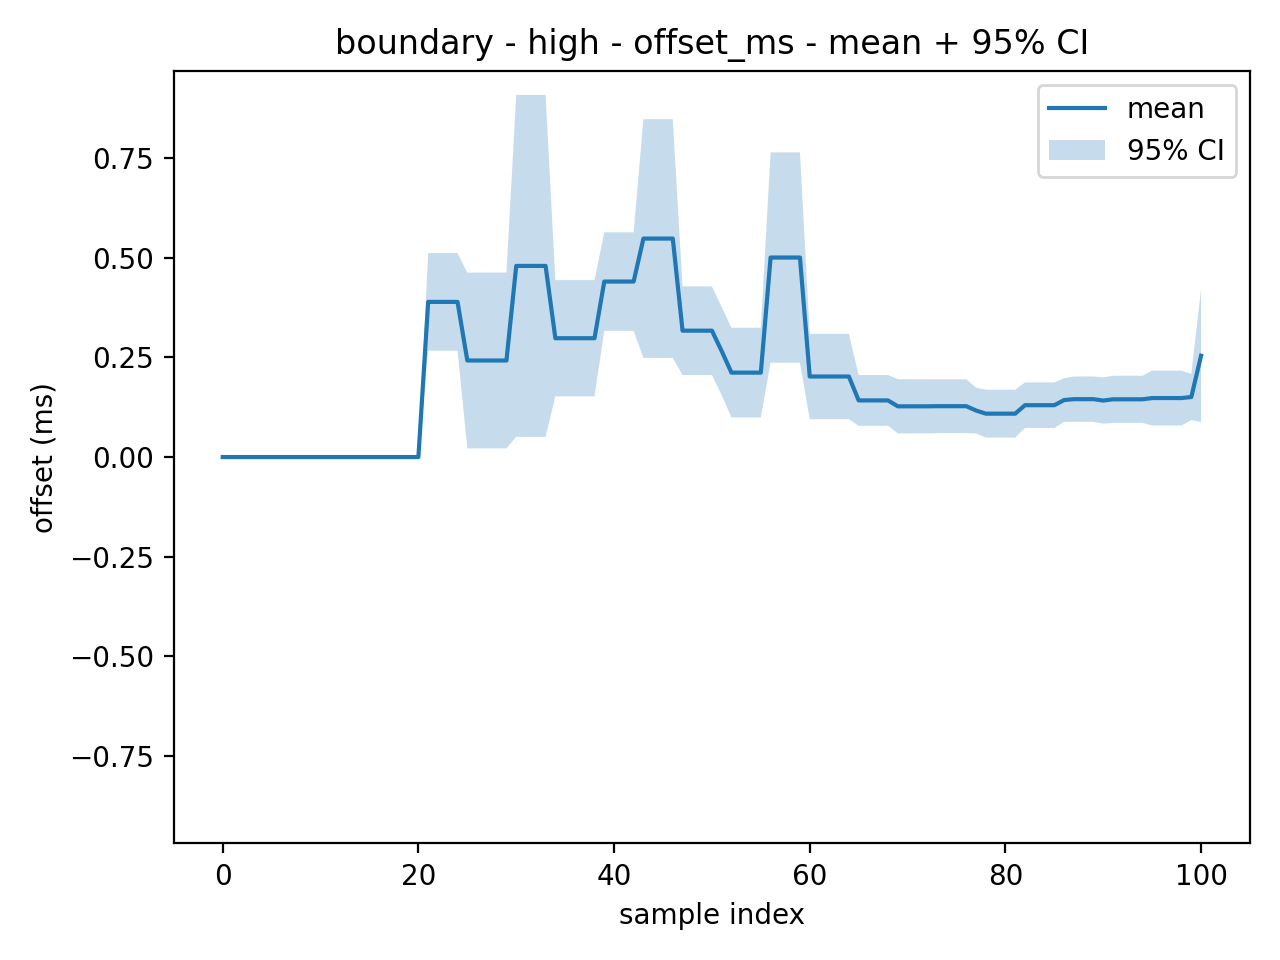
\includegraphics[width=\linewidth]{
      pars_plots/ntpsec/_aggregated/boundary/high/offset_ms_mean_ci95.png
    }
    \caption{Scenario HIGH}
  \end{subfigure}

  \caption{Media con intervallo di confidenza al 95\% - nodo: \texttt{boundary} metrica:
  \texttt{offset}}
  \label{fig:scenario_comparison}
\end{figure}
\begin{figure}[H]
  \centering

  \begin{subfigure}
    {0.32\textwidth}
    \centering
    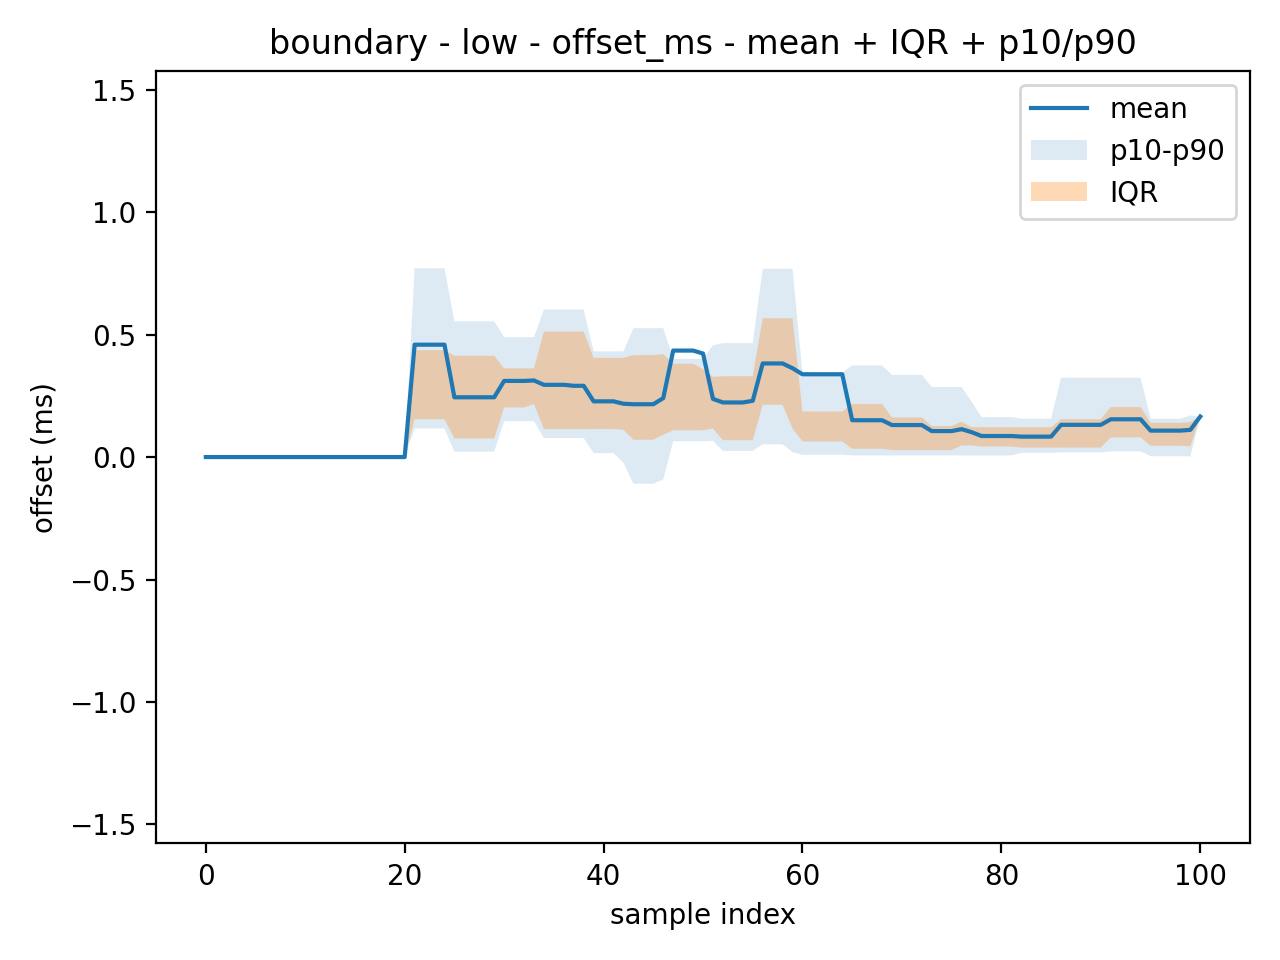
\includegraphics[width=\linewidth]{
      pars_plots/ntpsec/_aggregated/boundary/low/offset_ms_mean_iqr_p10_p90.png
    }
    \caption{Scenario LOW}
  \end{subfigure}
  \hfill
  \begin{subfigure}
    {0.32\textwidth}
    \centering
    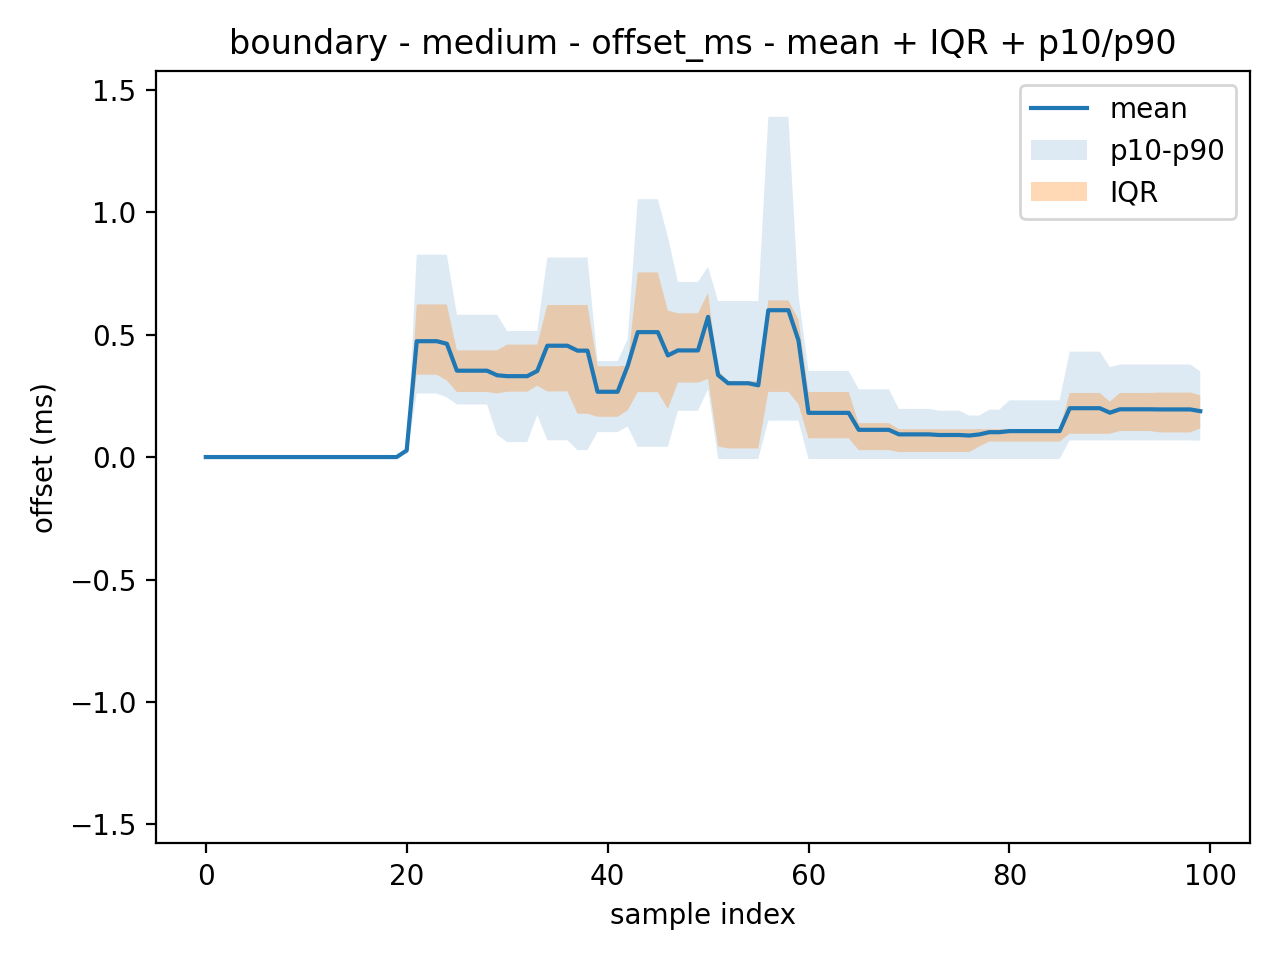
\includegraphics[width=\linewidth]{
      pars_plots/ntpsec/_aggregated/boundary/medium/offset_ms_mean_iqr_p10_p90.png
    }
    \caption{Scenario MEDIUM}
  \end{subfigure}
  \hfill
  \begin{subfigure}
    {0.32\textwidth}
    \centering
    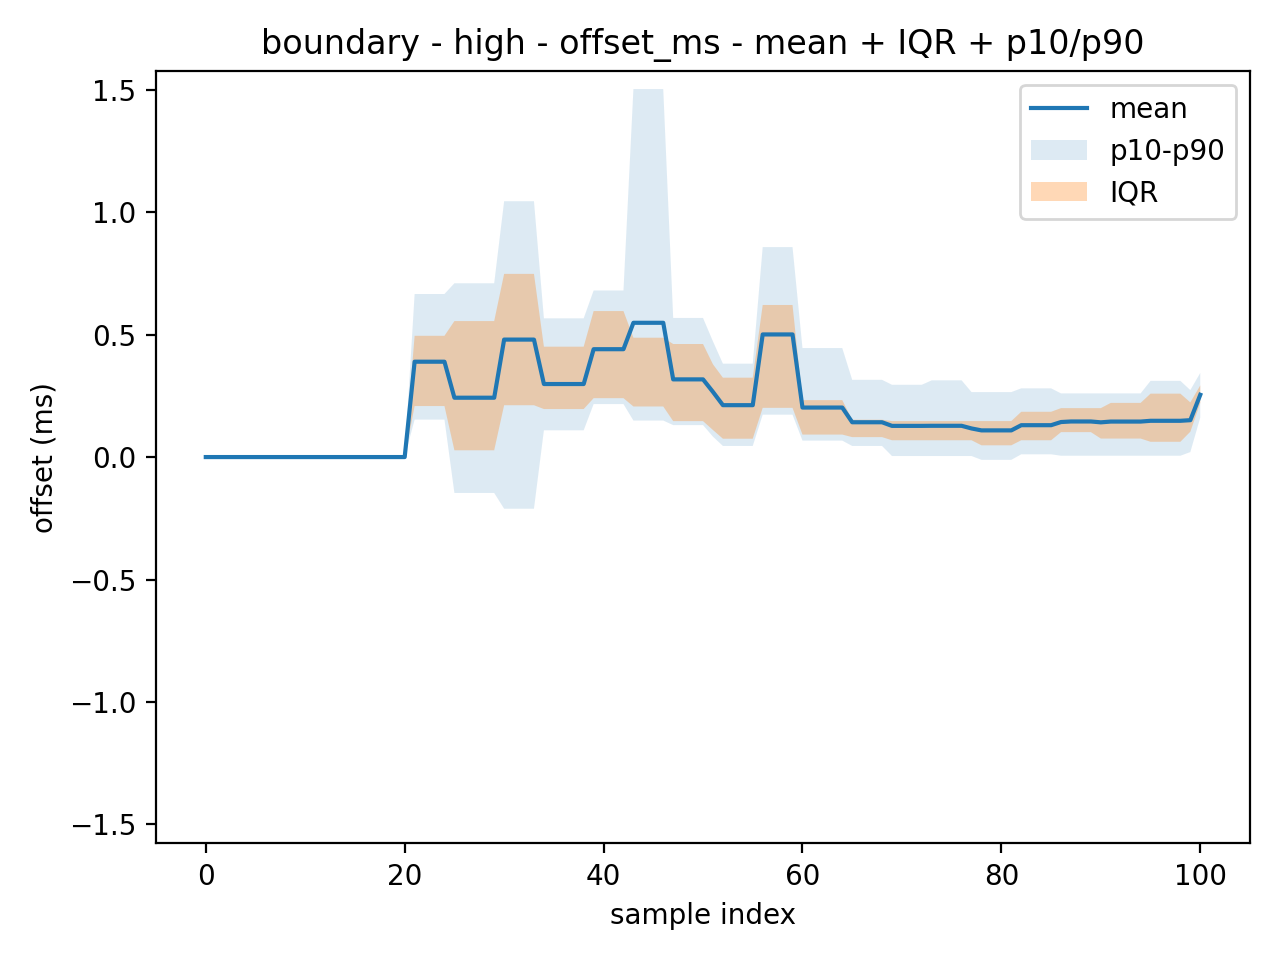
\includegraphics[width=\linewidth]{
      pars_plots/ntpsec/_aggregated/boundary/high/offset_ms_mean_iqr_p10_p90.png
    }
    \caption{Scenario HIGH}
  \end{subfigure}

  \caption{Media con banda inter-quartile e banda p10-p90 - nodo: \texttt{boundary}
  metrica: \texttt{offset}}
  \label{fig:scenario_comparison}
\end{figure}

Le metriche rilevate evidenziano un comportamento notevolmente differente
rispetto a quelle osservate sul nodo client. In tutti e tre gli scenari i dati restano
coerenti e stabili, con valori dello stesso ordine di grandezza, non evidenziando
una crescita progressiva netta al crescere della severità degli impairment di rete.
Vi è coerenza con la premessa iniziale.

Il delay ha valori medi di ~1.080 ms nello scenario low, ~1.139 ms nello scenario
medium e ~1.127 ms nello scenario high. Variazioni minime che non configurano un cambio
di regime. La dispersione associata conferma le ipotesi, con metriche dello stesso
ordine di grandezza.

Andamento analogo è osservabile per il jitter. I valori medi sono di circa 0.446
ms in low, 0.442 ms in medium e 0.473 ms in high. Differenze ridotte, evidenziando
un'assenza di degrado del nodo \texttt{boundary}.La variabilità delle curve
aggregate resta limitata, suggerendo un comportamento omogeneo nei tre casi.

Infine l'offset, con valori anche essi contenuti in tutti gli scenari. La media di
~0.204 ms nel caso low, 0.254 ms nel caso medium e 0.236 ms nel caso high.
Comportamento invariato, anche per la dispersione, con minime oscillazioni
compatibili con l'ambiente sperimentale, ma non un andamento monotono né un incremento
compatibile con un peggioramento strutturale.

I risultati ottenuti mostrano quindi un assenza di degrado. Le differenze
osservate tra low, medium e high risultano contenute e prive di una tendenza sistematica,
confermando l'ipotesi iniziale.

\section{\texttt{ptp4l}}
L'analisi dei dati relativa al demone \texttt{\textbf{ptp4l}} è fatta su due nodi
della topologia. In particolare sui nodi \texttt{clientptp} e \texttt{boundary}, per
i quali sono disponibili misurazioni direttamente riconducibili al comportamento del
protocollo in termini di sincronizzazione e ritardo.

Il nodo \texttt{servergm}, per configurazione, essendo eletto definitivamente GM,
non fornisce metriche comparabili, poiché il relativo output è limitato
essenzialmente allo stato di inizializzazione del demone e alla selezione del
clock locale come \texttt{best master}, non viene quindi incluso nell'analisi.

Anche in questa situazione \texttt{\textbf{ptp4l}}, gli impairment di rete
introdotti mediante \texttt{tc/netem} sono applicati sul ramo \texttt{downstream}
a valle del nodo \texttt{boundary}. Di conseguenza il confronto tra scenari
assume significato principalmente nel caso del nodo \texttt{clientptp}. Per
quanto riguarda il nodo \texttt{boundary} ci si attende, in linea teorica, un impatto
più contenuto, o una totale assenza di degrado.

Alla luce di ciò, l'analisi viene sviluppata separatamente per i nodi \texttt{clientptp}
e \texttt{boundary}.

\subsection{\texttt{clientptp}}
Per quanto riguarda, l'analisi quantitativa delle metriche, non può essere estesa
in modo uniforme a tutti gli scenari. Infatti, nello scenario \texttt{high} non
venendo raggiunta una stabile condizione operativa i campioni prodotti non sono
utilizzabili per un confronto. Quindi l'analisi si limita agli scenari \texttt{low}
e \texttt{medium}.

L'instabilità non raggiunta è evidenziata dal file di log, il quale mostra
ripetute selezioni del clock locale come miglior master e un solo tentativo
transitorio di passaggio verso un master esterno, seguito tuttavia da ritorno allo
stato di \texttt{LISTENING}. L'assenza di campioni numerici confrontabili nello scenario
\texttt{high} rappresenta dunque un risultato sperimentale, e segnala un livello di
degrado tale da impedire la normale operatività del client PTP. Il relativo
output viene comunque richiamato a supporto di tale evidenza qualitativa.

\subsubsection{Analisi metrica: \texttt{path Delay}}
\begin{figure}[H]
  \centering

  \begin{subfigure}
    {0.4\textwidth}
    \centering
    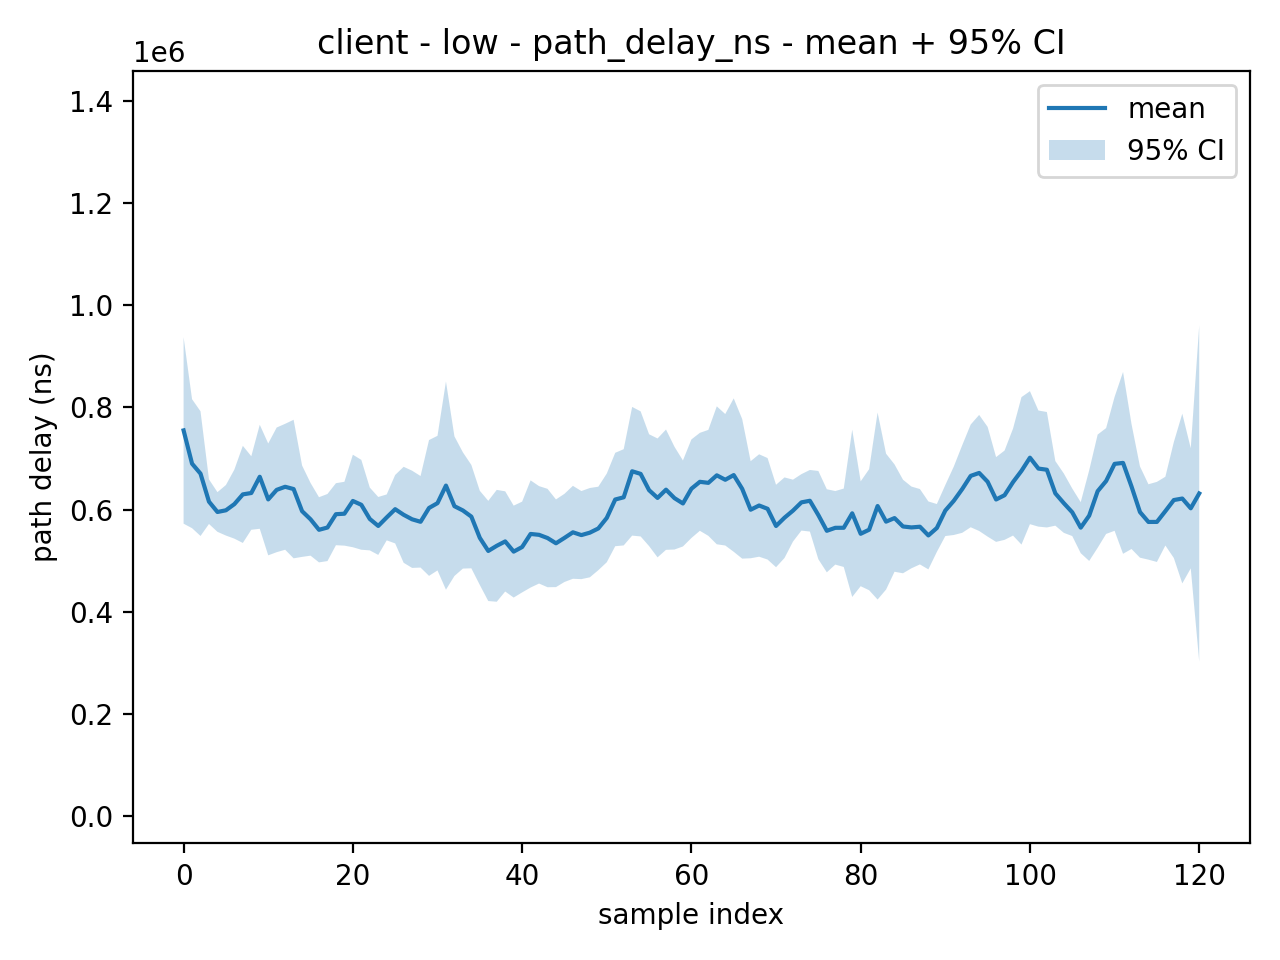
\includegraphics[width=\linewidth]{
      pars_plots/ptp/_aggregated/client/low/path_delay_ns_mean_ci95.png
    }
    \caption{Scenario LOW}
  \end{subfigure}
  \hfill
  \begin{subfigure}
    {0.4\textwidth}
    \centering
    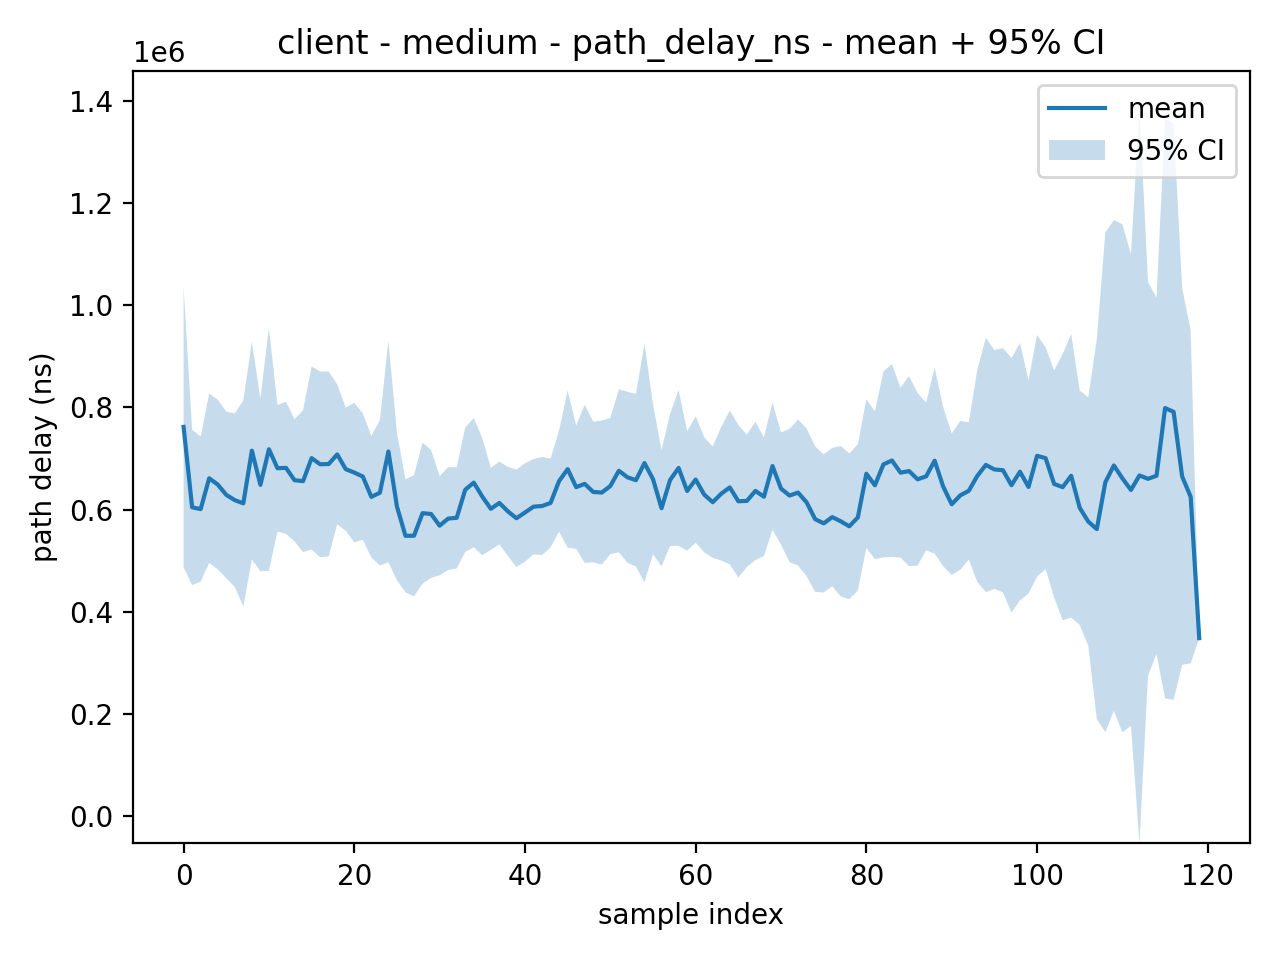
\includegraphics[width=\linewidth]{
      pars_plots/ptp/_aggregated/client/medium/path_delay_ns_mean_ci95.png
    }
    \caption{Scenario MEDIUM}
  \end{subfigure}
  \caption{Media con intervallo di confidenza al 95\% - nodo: \texttt{clientptp}}
  \label{fig:scenario_comparison}
\end{figure}
\begin{figure}[H]
  \centering

  \begin{subfigure}
    {0.4\textwidth}
    \centering
    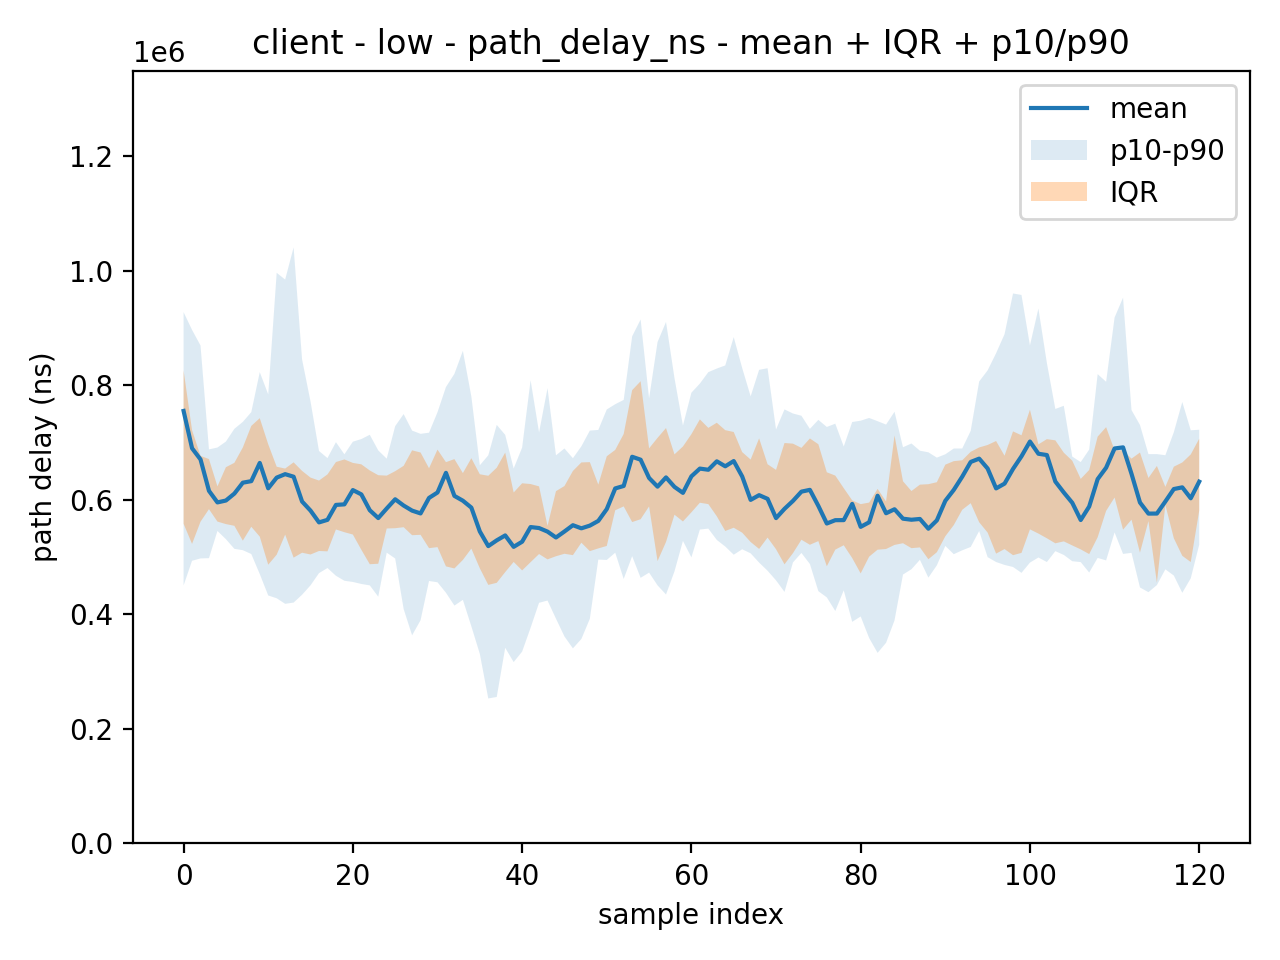
\includegraphics[width=\linewidth]{
      pars_plots/ptp/_aggregated/client/low/path_delay_ns_mean_iqr_p10_p90.png
    }
    \caption{Scenario LOW}
  \end{subfigure}
  \hfill
  \begin{subfigure}
    {0.4\textwidth}
    \centering
    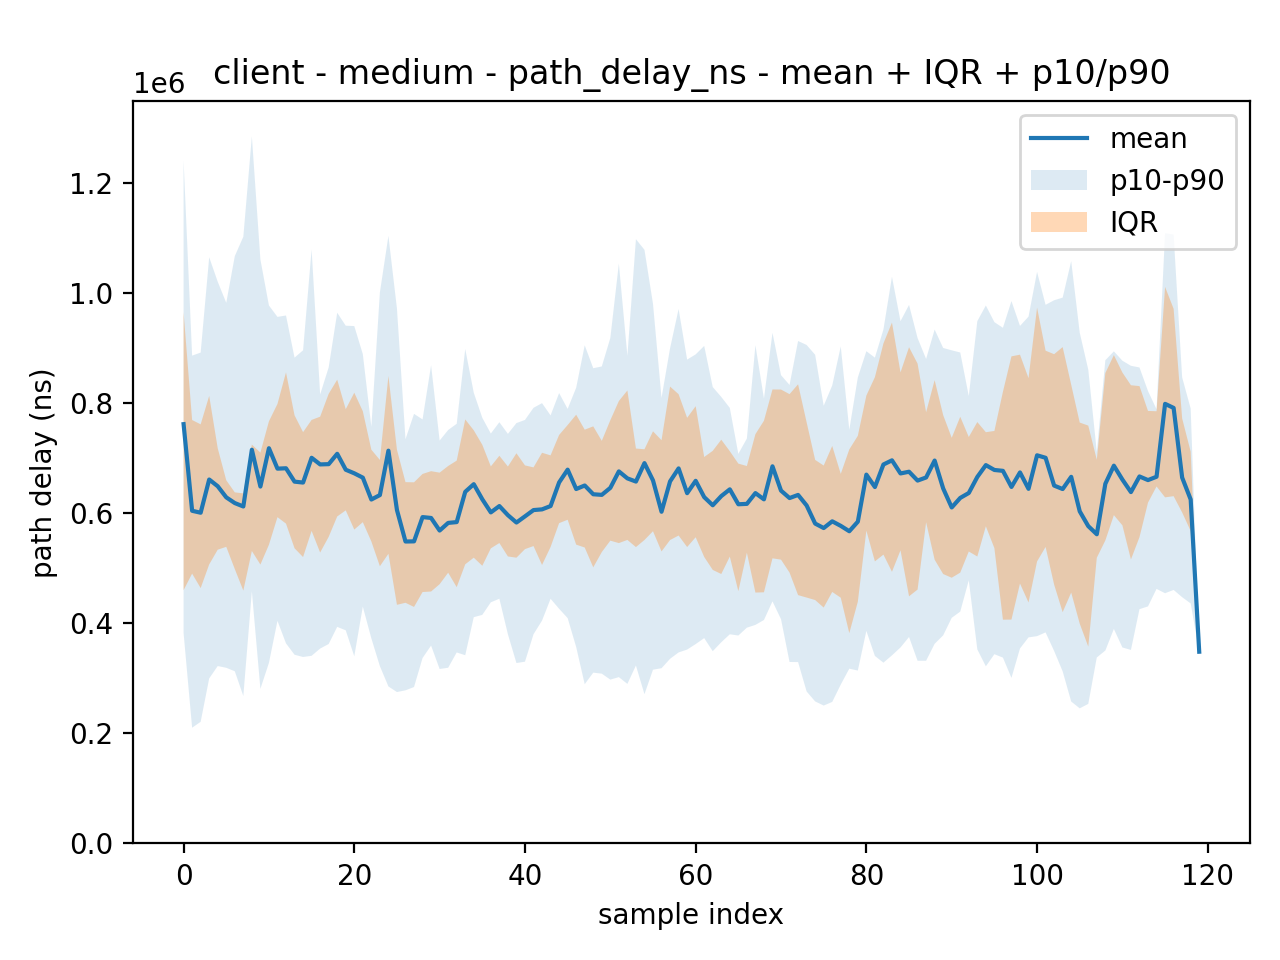
\includegraphics[width=\linewidth]{
      pars_plots/ptp/_aggregated/client/medium/path_delay_ns_mean_iqr_p10_p90.png
    }
    \caption{Scenario MEDIUM}
  \end{subfigure}
  \caption{Media con banda inter-quartile e banda p10-p90 - nodo: \texttt{clientptp}}
  \label{fig:scenario_comparison}
\end{figure}

La metrica \texttt{path delay} sul nodo \texttt{clientptp} consente di valutare il
ritardo stimato lungo il percorso di sincronizzazione tra il client e il master.

Nello scenario \texttt{low} vi è un andamento mediamente regolare, collocandosi su
valori nell'ordine di centinaia di microsecondi. La curva aggregata ha un valore
medio ~$606.8\,\mu s$ e la mediana è di ~$602.5\,\mu s$. La distribuzione dei valori
centrali è piuttosto contenuta, con il primo e terzo quartile rispettivamente a
$575.8\,\mu s$ e $638.6\,\mu s$. L'analisi dei grafici conferma un andamento stabile,
pur con oscillazioni locali non trascurabili, ma complessivamente compatibili con
una condizione di rete moderatamente controllata.

Nel caso \texttt{medium}, si ha un livello medio crescente ma sempre contenuto.
La curva aggregata ha un valore medio di ~$6 42.2\,\mu s$, con mediana pari a ~$6
45 .5\,\mu s$. L'incremento rispetto allo scenario precedente è nell'ordine di
decine di microsecondi. Questo scenario, comunque, mostra una dispersione più elevata.
Il primo e il terzo quartile della curva centrale sono rispettivamente pari a
$613.0\,\mu s$ e $672.3\, \mu s$, invece le bande di variabilità sono mediamente più
ampie. L'ampiezza dell'IQR, cosi come quella della fascia $p10$--$p 90$, segnalano una
minore regolarità della stima del ritardo di percorso.

Vi è un chiaro aumento del degrado tra i primi due scenari, in termini di misurazioni
ottenute. Nonostante il degrado della rete non produce un forte aumento del
valore medio del \texttt{path delay}, ma si riflette soprattutto in una maggiore
variabilità delle misurazioni. La metrica risulta quindi sensibile al peggioramento
dello scenario sperimentale, ma l'effetto osservato si manifesta principalmente
come perdita di stabilità più che come incremento netto del livello centrale. Lo scenario
\texttt{high}, come già discusso, evidenzia una totale perdita di connessione
con il riferimento principale.

\subsubsection{Analisi metrica: \texttt{RMS offset}}
\begin{figure}[H]
  \centering

  \begin{subfigure}
    {0.4\textwidth}
    \centering
    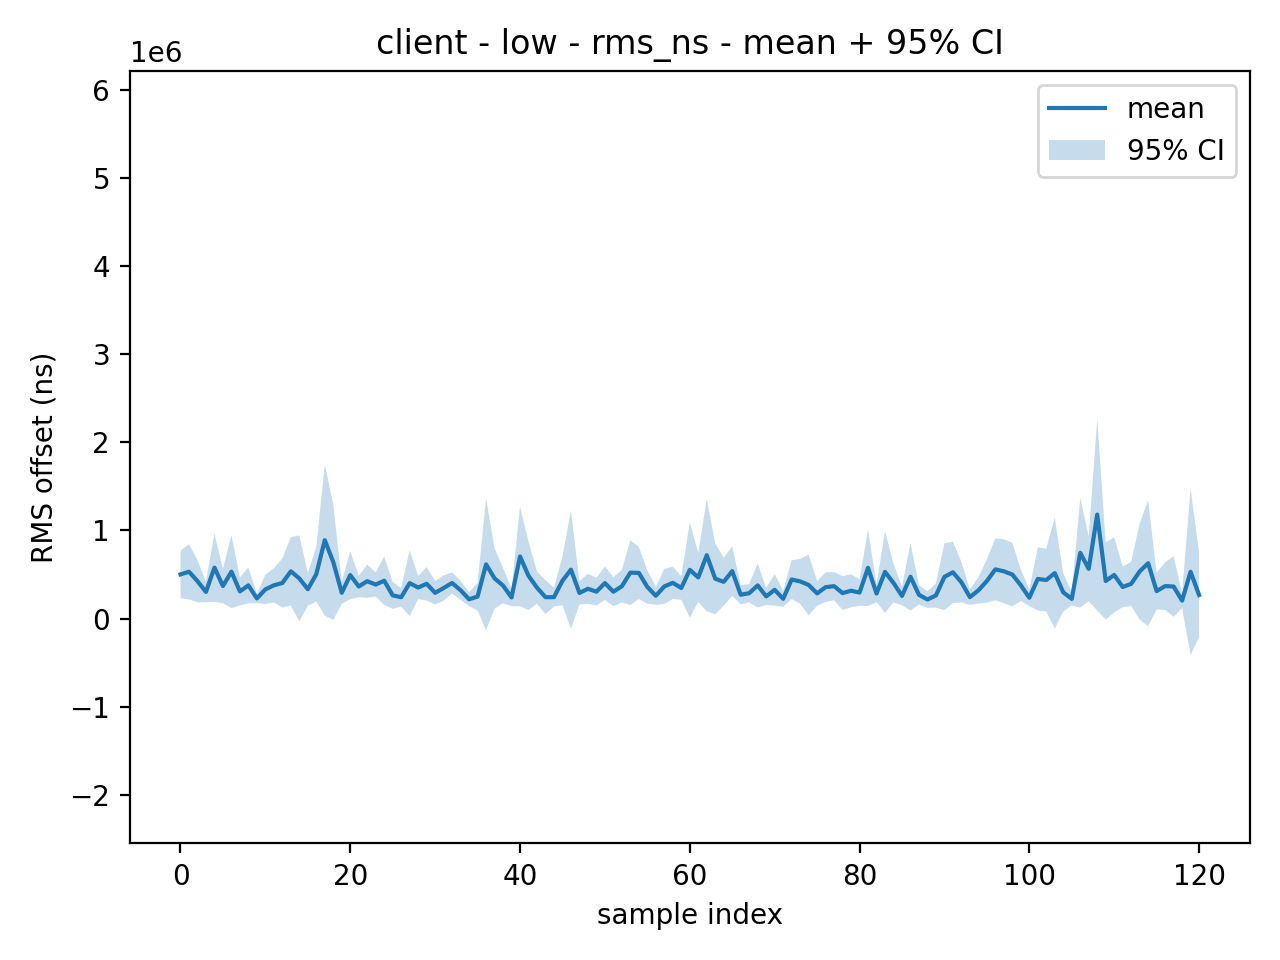
\includegraphics[width=\linewidth]{
      pars_plots/ptp/_aggregated/client/low/rms_ns_mean_ci95.png
    }
    \caption{Scenario LOW}
  \end{subfigure}
  \hfill
  \begin{subfigure}
    {0.4\textwidth}
    \centering
    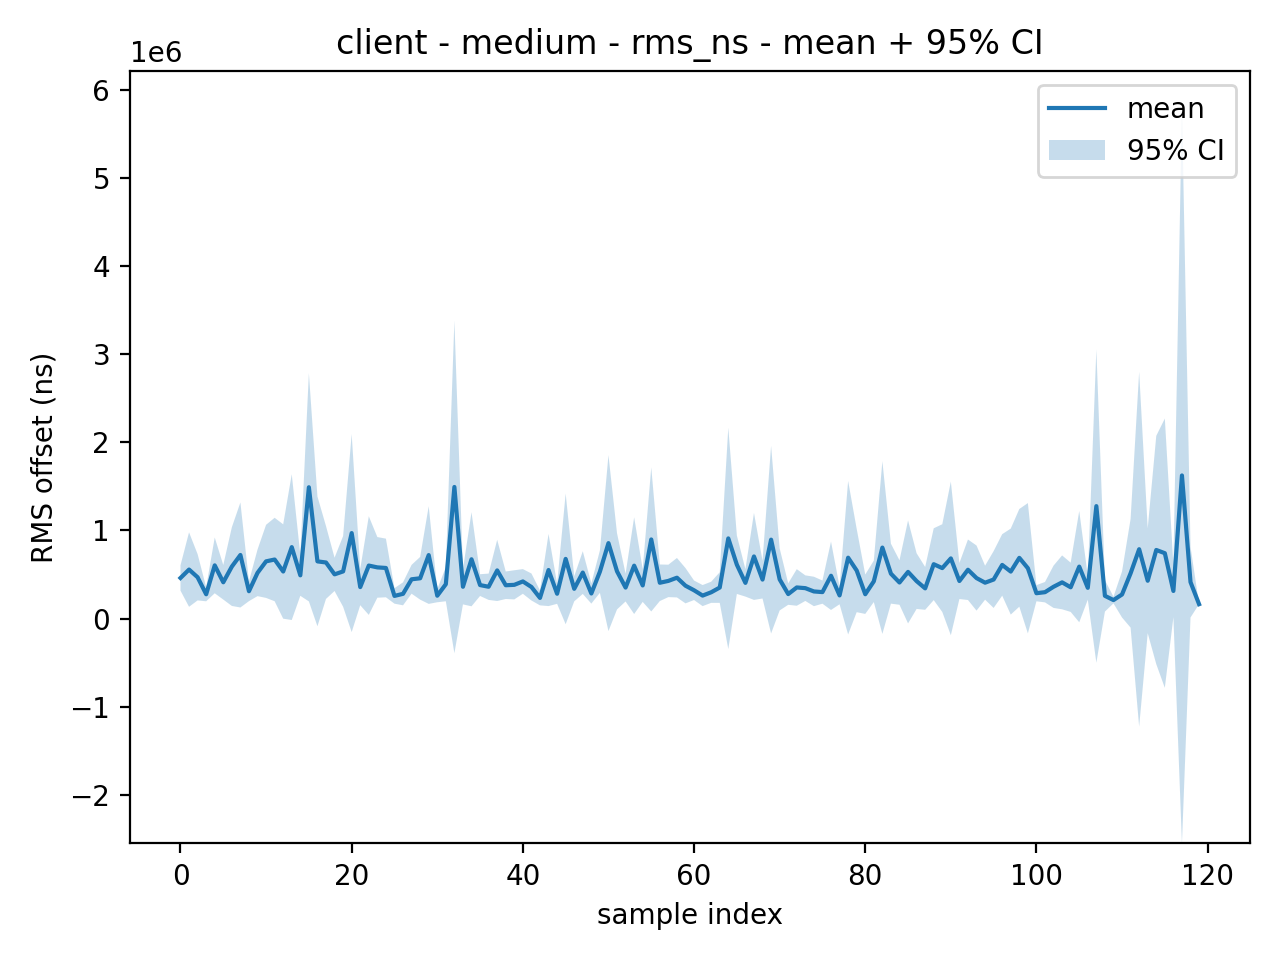
\includegraphics[width=\linewidth]{
      pars_plots/ptp/_aggregated/client/medium/rms_ns_mean_ci95.png
    }
    \caption{Scenario MEDIUM}
  \end{subfigure}
  \caption{Media con intervallo di confidenza al 95\% - nodo: \texttt{clientptp}}
  \label{fig:scenario_comparison}
\end{figure}
\begin{figure}[H]
  \centering

  \begin{subfigure}
    {0.4\textwidth}
    \centering
    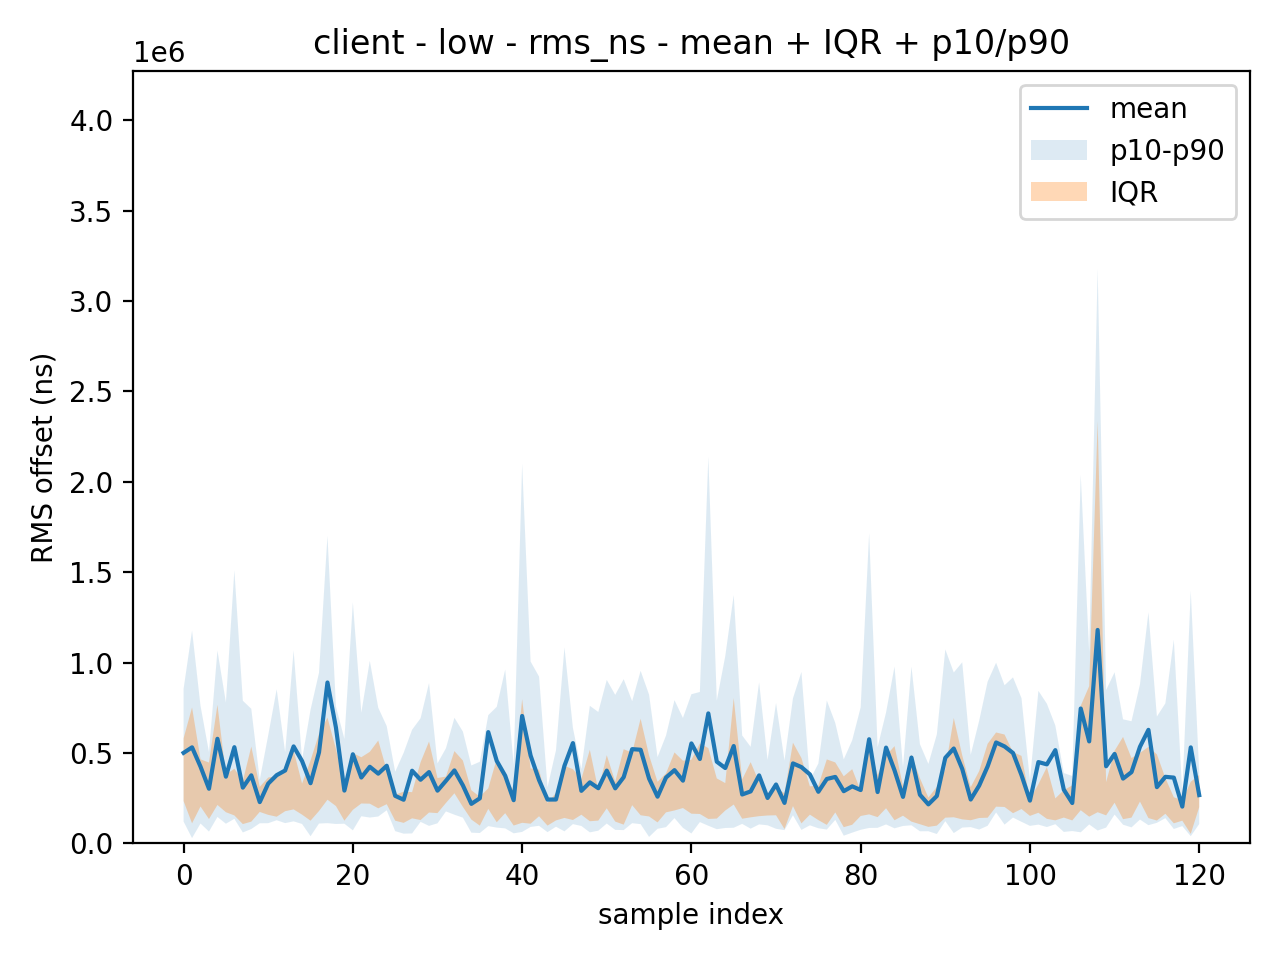
\includegraphics[width=\linewidth]{
      pars_plots/ptp/_aggregated/client/low/rms_ns_mean_iqr_p10_p90.png
    }
    \caption{Scenario LOW}
  \end{subfigure}
  \hfill
  \begin{subfigure}
    {0.4\textwidth}
    \centering
    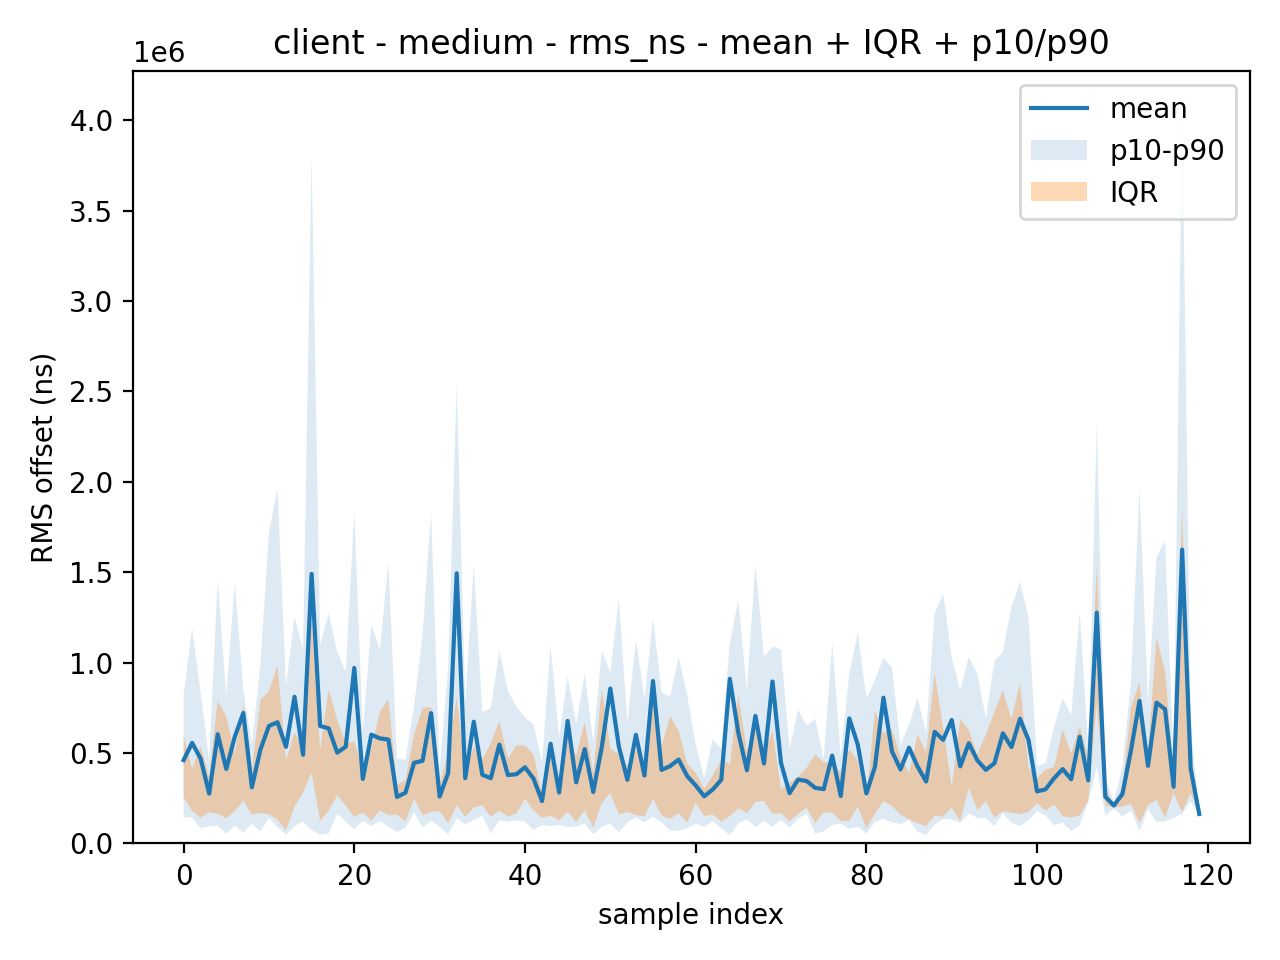
\includegraphics[width=\linewidth]{
      pars_plots/ptp/_aggregated/client/medium/rms_ns_mean_iqr_p10_p90.png
    }
    \caption{Scenario MEDIUM}
  \end{subfigure}
  \caption{Media con banda inter-quartile e banda p10-p90 - nodo: \texttt{clientptp}}
  \label{fig:scenario_comparison}
\end{figure}

La metrica \texttt{RMS} sul nodo \texttt{clientptp} misura l'entità media dell'errore
di sincronizzazione osservato dal client PTP fornendo una misura della qualità temporale
raggiunta dal nodo nel corso dell'esperimento.

Nello scenario \texttt{low}, i valori medi sono nell'ordine di alcune centinaia di
microsecondi. Il valore medio della curva aggregata è di ~$406.7\,\mu s$, mentre
la mediana è ~$378.1\,\mu s$. La distribuzione dei valori centrali è nell'intervallo
$3 02.5\,\mu s$ e $493.2\,\mu s$, con presenza di picchi locali più elevati.
L'andamento della serie risulta nel complesso irregolare ma ancora contenuto.

Nello scenario \texttt{medium}, la RMS aumenta. Il valore medio della curva aggregata
si attesta a ~$514.9\,\mu s$. La mediana ha un valore di ~$458.5\,\mu s$. Rispetto
allo scenario \texttt{low} vi è un incremento sensibile pari a poco più di
$100\,\mu s$. L'aspetto però più rilevante è rappresentato dall'aumento della dispersione.
L'intervallo inter-quartile dei valori centrali è maggiore e le bande di
variabilità nei grafici risultano più estese. In generale la serie mostra una maggiore
oscillazione.

In generale, la metrica RMS mostra un marcato peggioramento al passaggio dallo
scenario \texttt{low} a quello \texttt{medium}. A differenza di quanto osservato sul
\texttt{path delay} vi è anche un incremento maggiore del livello medio
dell'errore temporale. Per lo scenario \texttt{high} vale sempre la premessa
iniziale, confermando l'eccessivo degrado di rete che non permette a \texttt{clientptp}
di stabilizzarsi.

\subsection{\texttt{boundary}}
L'analisi sul nodo \texttt{boundary} è simmetrica a quella effettuata con il demone
\texttt{NTPsec}. Le metriche osservate in questo caso descrivono infatti il comportamento
della sincronizzazione del boundary rispetto al \texttt{master upstream} (\texttt{servergm}).
Non essendoci impairment di rete direttamente applicati, in linea teorica, non
ci si attende un degrado strutturale. A sostegno dell'ipotesi vi è la presenza dei
dati osservati anche nello scenario \texttt{high}.

Occorre tuttavia considerare che il demone \texttt{ptp4l} opera sul nodo in modo unitario,
gestendo contemporaneamente più porte della topologia. Per tale ragione,
eventuali fault, transizioni di stato o condizioni di instabilità osservate sulla
porta downstream possono comunque riflettersi indirettamente sulla stabilità complessiva
del processo di sincronizzazione, introducendo fluttuazioni o anomalie anche
nelle metriche riferite al tratto upstream. L'analisi che segue è pertanto finalizzata
a verificare se i dati confermino una sostanziale stabilità del nodo \texttt{boundary}
nei tre scenari sperimentali, oppure se emergano effetti indiretti riconducibili alle
criticità operative osservate durante il testing.

\subsubsection{Analisi metrica: \texttt{path delay}}
\begin{figure}[H]
  \centering

  \begin{subfigure}
    {0.32\textwidth}
    \centering
    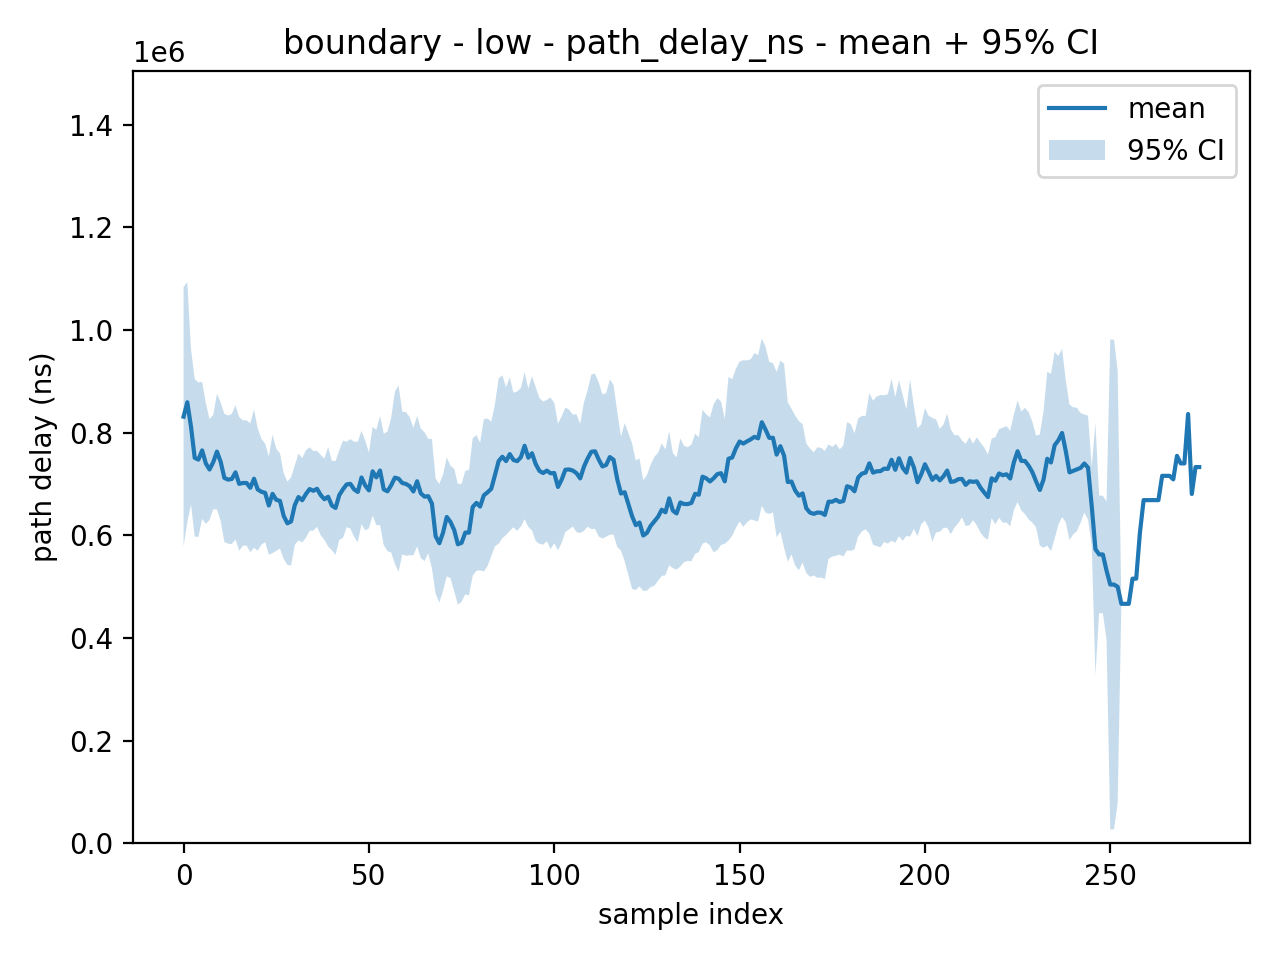
\includegraphics[width=\linewidth]{
      pars_plots/ptp/_aggregated/boundary/low/path_delay_ns_mean_ci95.png
    }
    \caption{Scenario LOW}
  \end{subfigure}
  \hfill
  \begin{subfigure}
    {0.32\textwidth}
    \centering
    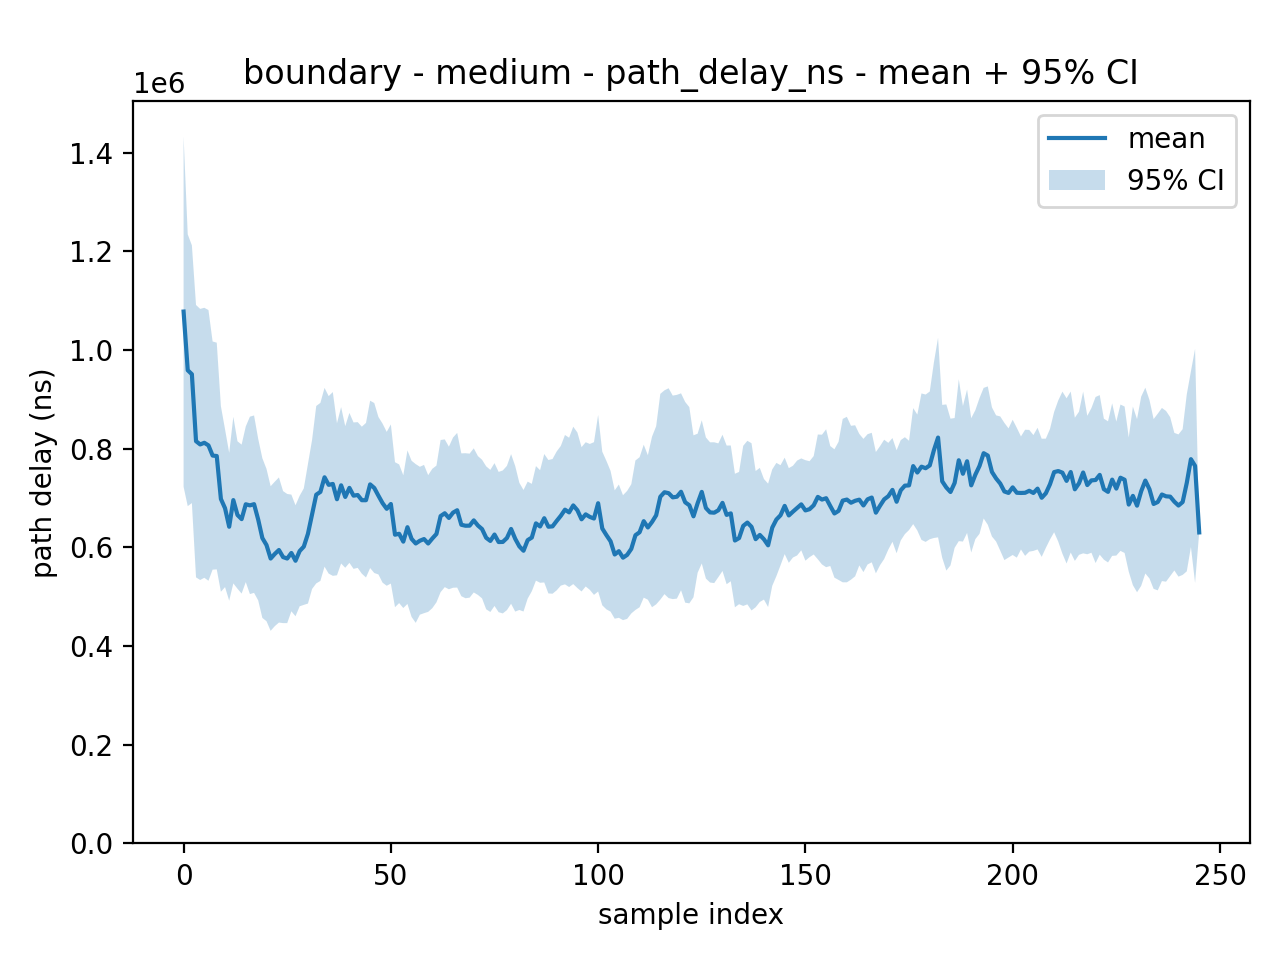
\includegraphics[width=\linewidth]{
      pars_plots/ptp/_aggregated/boundary/medium/path_delay_ns_mean_ci95.png
    }
    \caption{Scenario MEDIUM}
  \end{subfigure}
  \begin{subfigure}
    {0.32\textwidth}
    \centering
    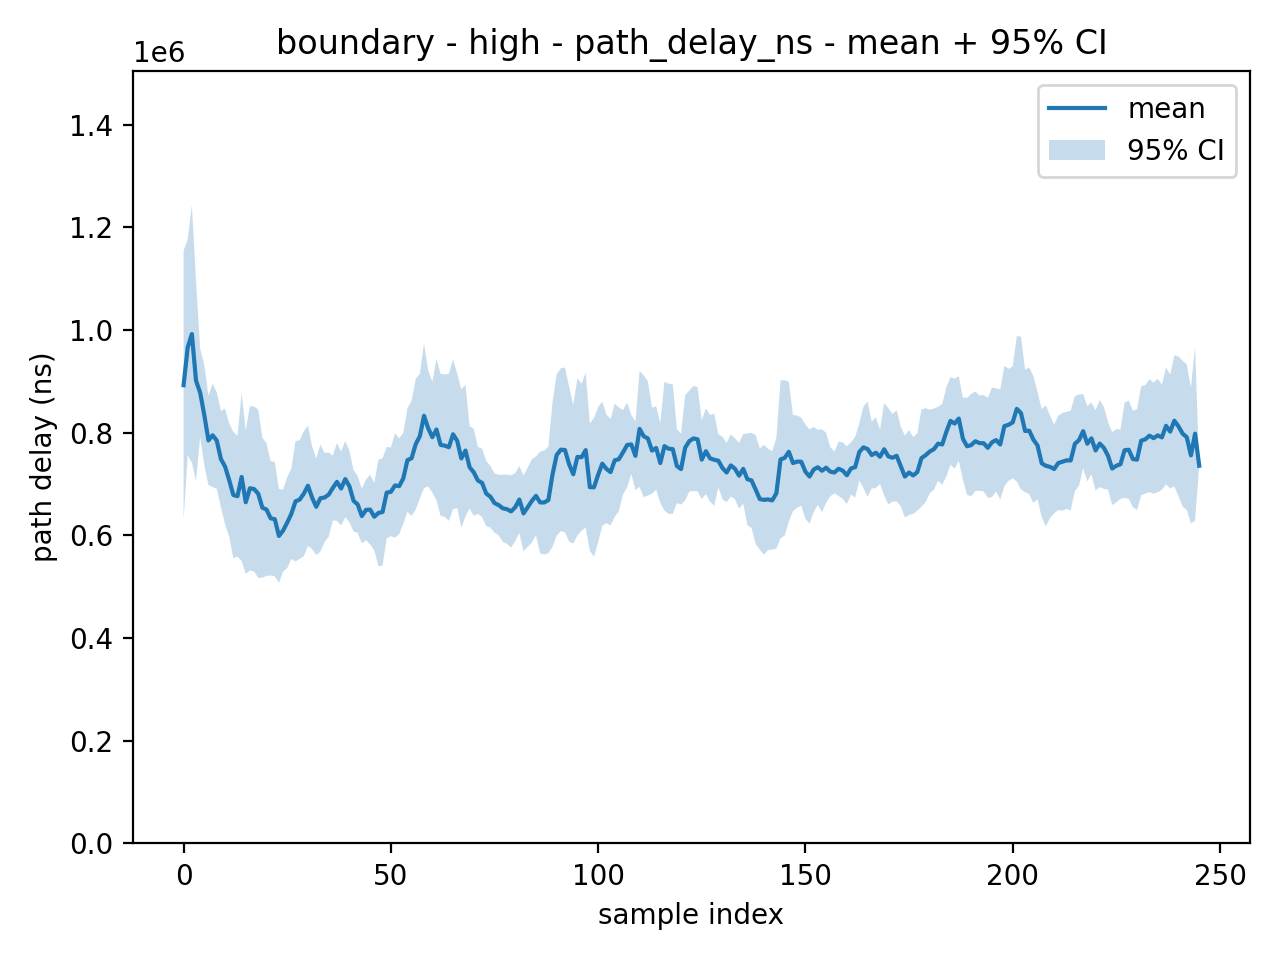
\includegraphics[width=\linewidth]{
      pars_plots/ptp/_aggregated/boundary/high/path_delay_ns_mean_ci95.png
    }
    \caption{Scenario HIGH}
  \end{subfigure}
  \caption{Media con intervallo di confidenza al 95\% - nodo: \texttt{boundary}}
  \label{fig:scenario_comparison}
\end{figure}
\begin{figure}[H]
  \centering

  \begin{subfigure}
    {0.32\textwidth}
    \centering
    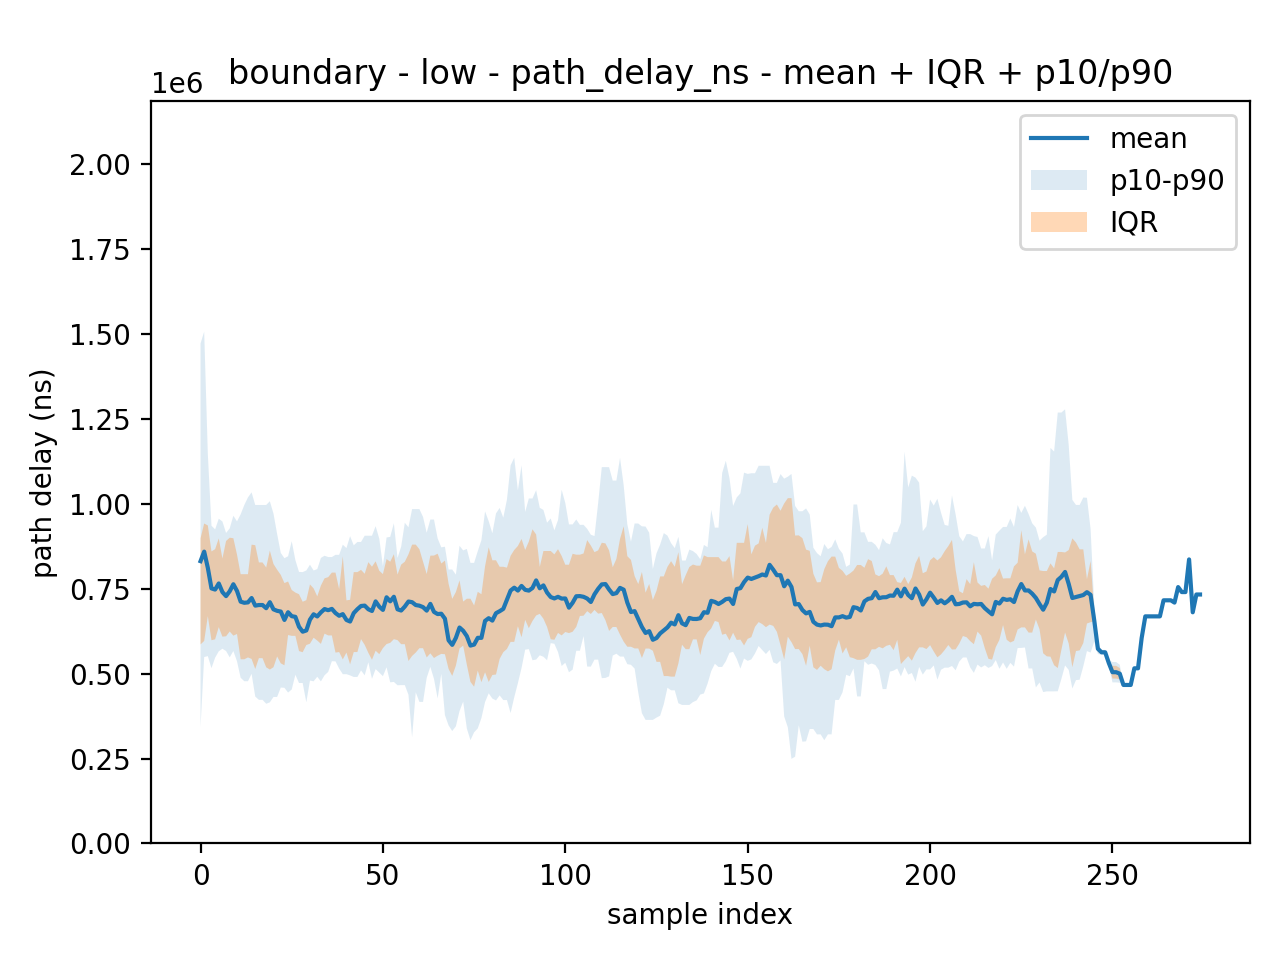
\includegraphics[width=\linewidth]{
      pars_plots/ptp/_aggregated/boundary/low/path_delay_ns_mean_iqr_p10_p90.png
    }
    \caption{Scenario LOW}
  \end{subfigure}
  \hfill
  \begin{subfigure}
    {0.32\textwidth}
    \centering
    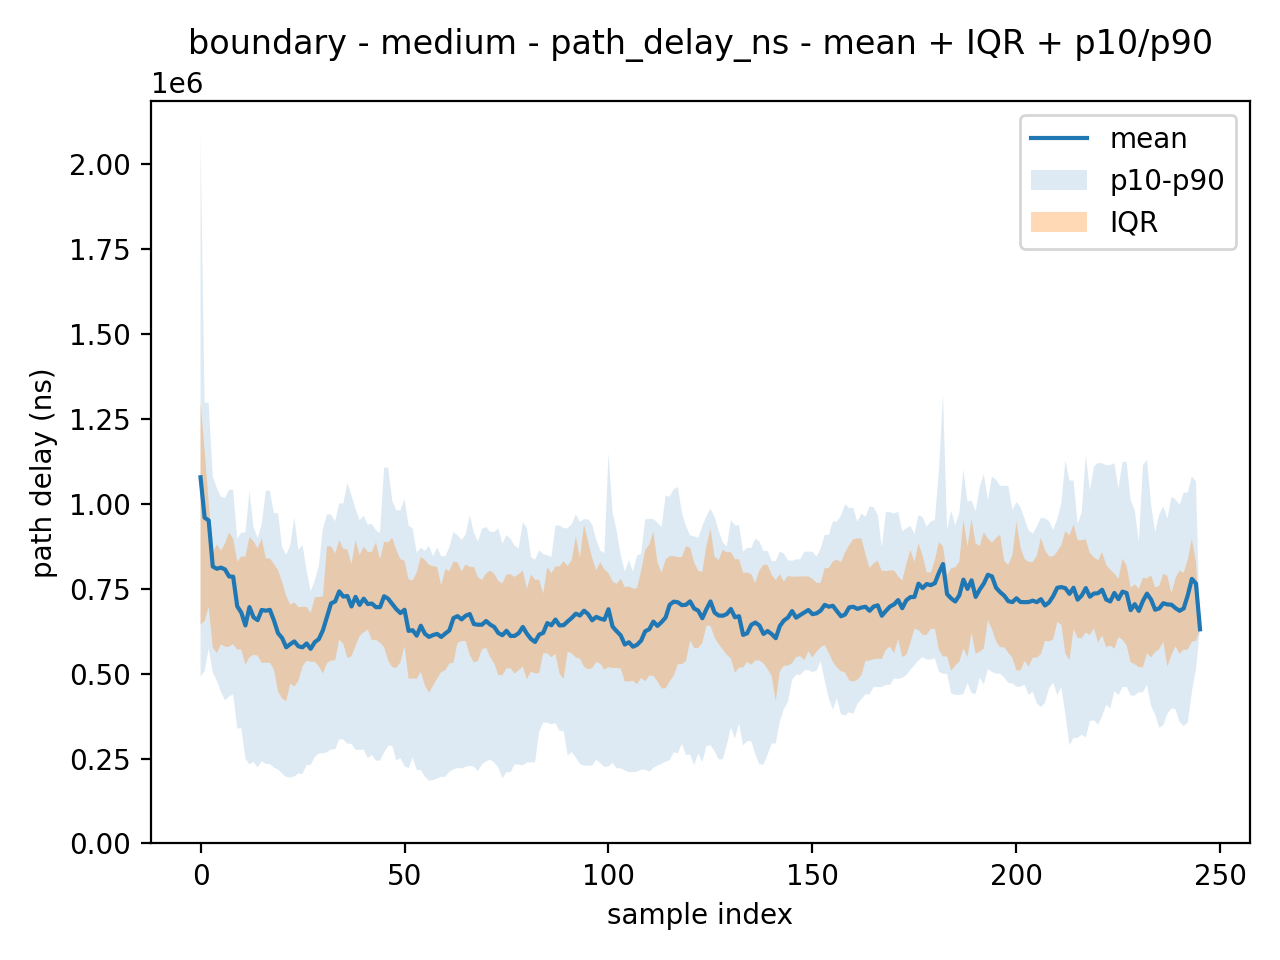
\includegraphics[width=\linewidth]{
      pars_plots/ptp/_aggregated/boundary/medium/path_delay_ns_mean_iqr_p10_p90.png
    }
    \caption{Scenario MEDIUM}
  \end{subfigure}
  \begin{subfigure}
    {0.32\textwidth}
    \centering
    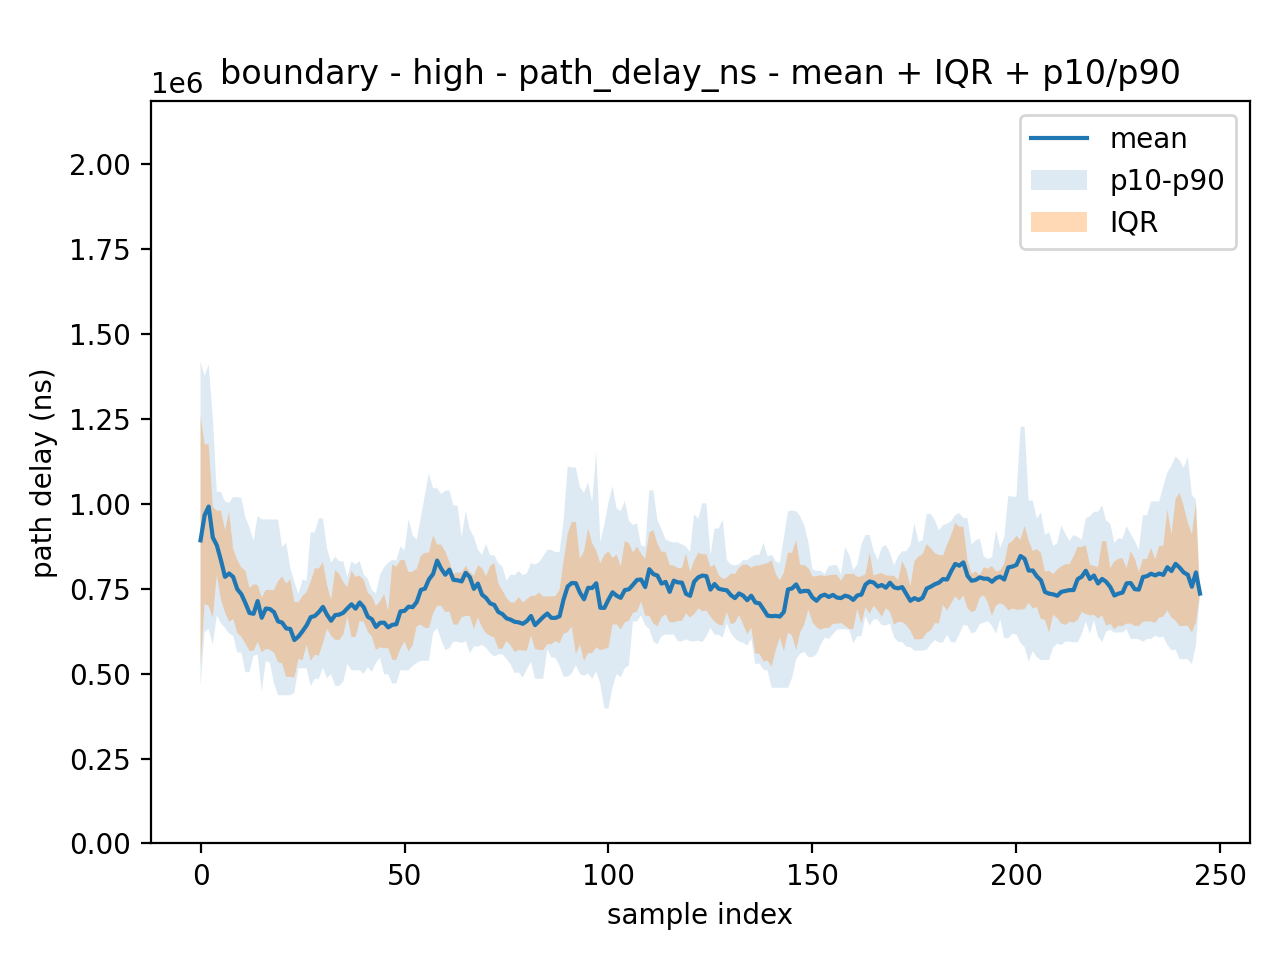
\includegraphics[width=\linewidth]{
      pars_plots/ptp/_aggregated/boundary/high/path_delay_ns_mean_iqr_p10_p90.png
    }
    \caption{Scenario HIGH}
  \end{subfigure}
  \caption{Media con banda inter-quartile e banda p10-p90 - nodo: \texttt{boundary}}
  \label{fig:scenario_comparison}
\end{figure}
Per quanto riguarda il \texttt{path delay} vi è conferma, nel complesso, dell'ipotesi.
Le tre condizioni sperimentali presentano infatti valori medi dello stesso ordine
di grandezza e profili temporali complessivamente regolari, senza evidenza di un
deterioramento sistematico e monotono.

Da un punto di vista quantitativo, si ha un valore medio aggregato del \texttt{path
delay} di ~697.227~\textmu s nello scenario \texttt{low}, 687.669~\textmu s nello
scenario \texttt{medium} e 740.415~\textmu s nello scenario \texttt{high}.
Differenze contenute nei tre casi, non indicano quindi una variazione sostanziale.
L'ampiezza inter-quartile media e la banda p10--p90 non mostrano infatti un incremento
progressivo e coerente con il livello di stress applicato.

Il grafico suggerisce, nello scenario \texttt{low} una curva media attorno a un stabile,
con eventuali fluttuazioni locali. Lo scenario \texttt{medium} mostra un
andamento particolarmente regolare nel tratto centrale, mentre nello scenario \texttt{high}
si osserva un innalzamento moderato del livello medio, comunque compatibile con una
condizione di sincronizzazione ancora stabile.

Per quanto riguarda la metrica del \texttt{path delay} c'è conferma sperimentale
dell'assenza di degrado strutturato. Le variazioni osservate possono essere interpretate
più plausibilmente come effetti indiretti del funzionamento complessivo del demone
\texttt{ptp4l}.

\subsubsection{Analisi metrica: \texttt{offset}}
\begin{figure}[H]
  \centering

  \begin{subfigure}
    {0.32\textwidth}
    \centering
    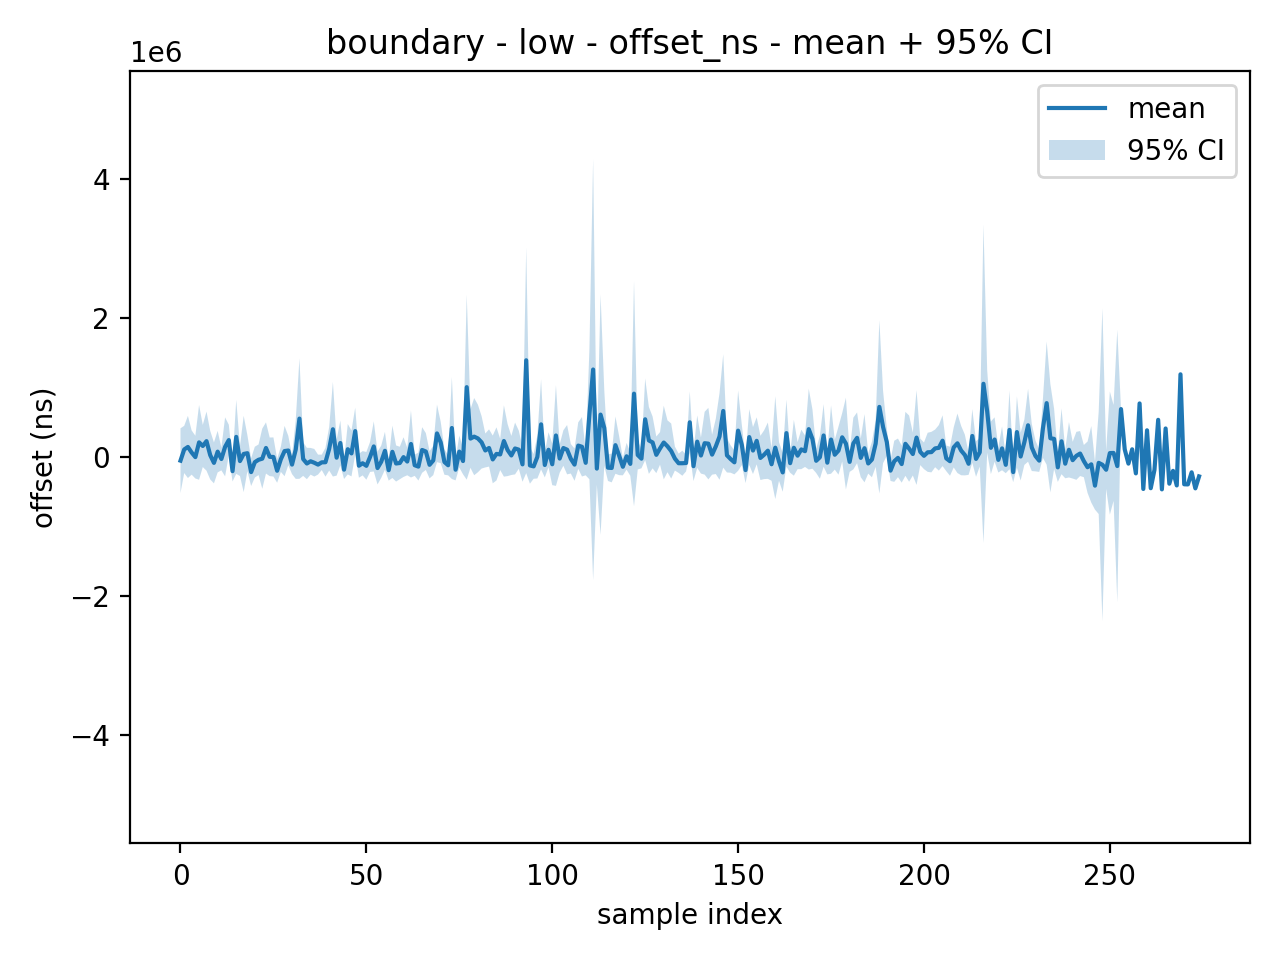
\includegraphics[width=\linewidth]{
      pars_plots/ptp/_aggregated/boundary/low/offset_ns_mean_ci95.png
    }
    \caption{Scenario LOW}
  \end{subfigure}
  \hfill
  \begin{subfigure}
    {0.32\textwidth}
    \centering
    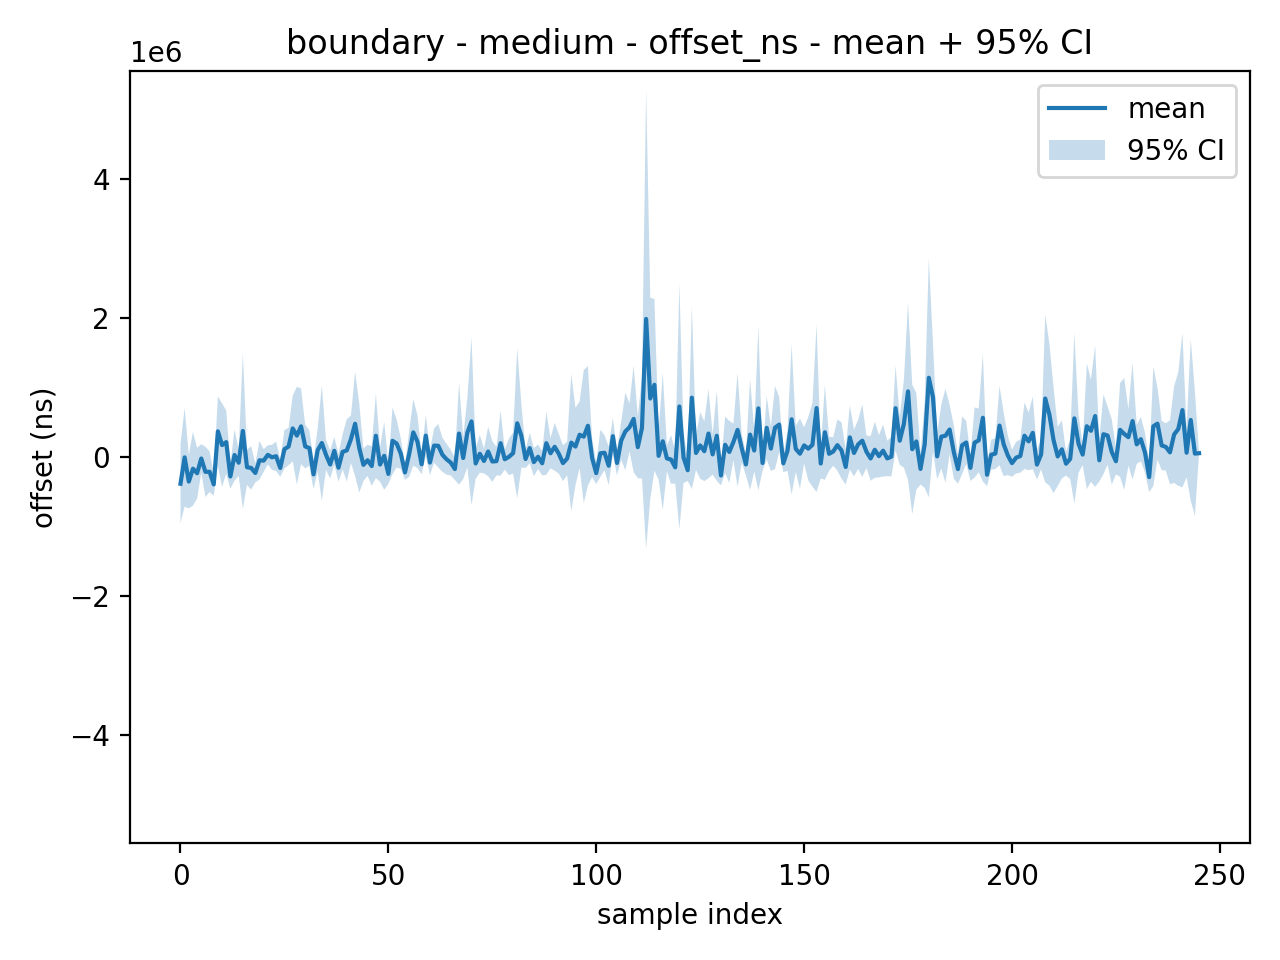
\includegraphics[width=\linewidth]{
      pars_plots/ptp/_aggregated/boundary/medium/offset_ns_mean_ci95.png
    }
    \caption{Scenario MEDIUM}
  \end{subfigure}
  \begin{subfigure}
    {0.32\textwidth}
    \centering
    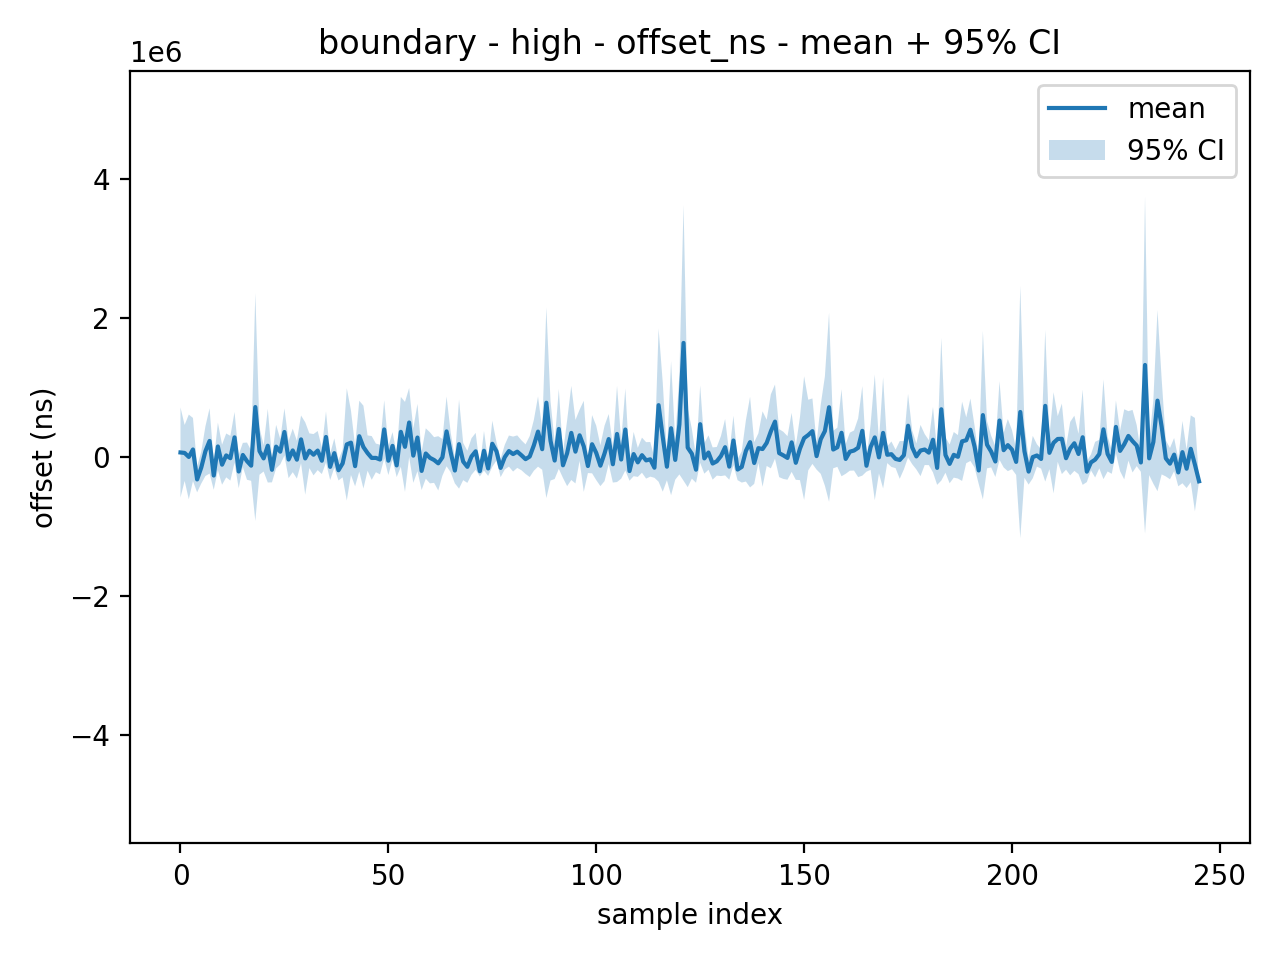
\includegraphics[width=\linewidth]{
      pars_plots/ptp/_aggregated/boundary/high/offset_ns_mean_ci95.png
    }
    \caption{Scenario HIGH}
  \end{subfigure}
  \caption{Media con intervallo di confidenza al 95\% - nodo: \texttt{boundary} -
  dati completi}
  \label{fig:scenario_comparison}
\end{figure}
\begin{figure}[H]
  \centering

  \begin{subfigure}
    {0.32\textwidth}
    \centering
    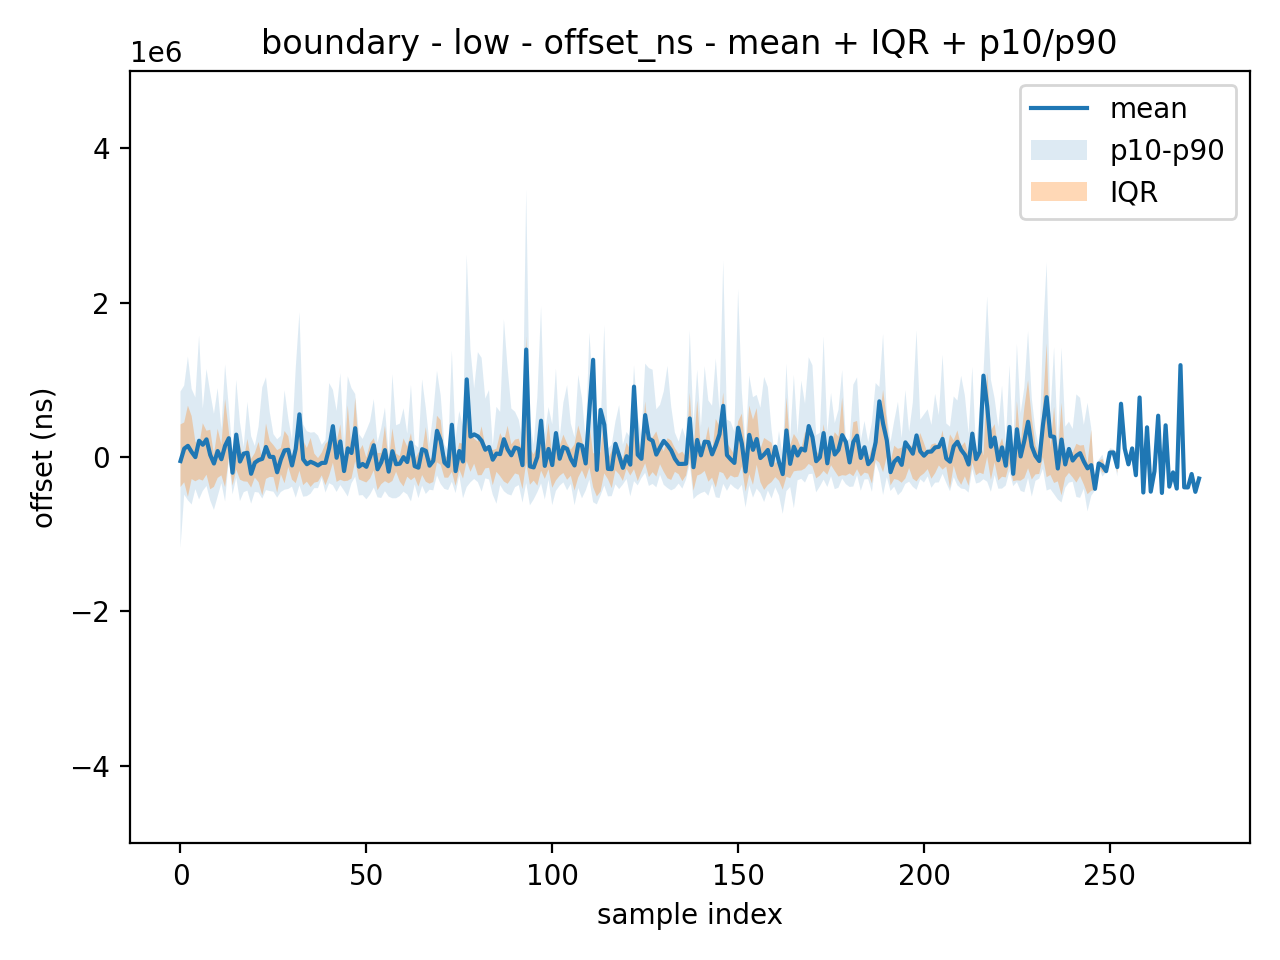
\includegraphics[width=\linewidth]{
      pars_plots/ptp/_aggregated/boundary/low/offset_ns_mean_iqr_p10_p90.png
    }
    \caption{Scenario LOW}
  \end{subfigure}
  \hfill
  \begin{subfigure}
    {0.32\textwidth}
    \centering
    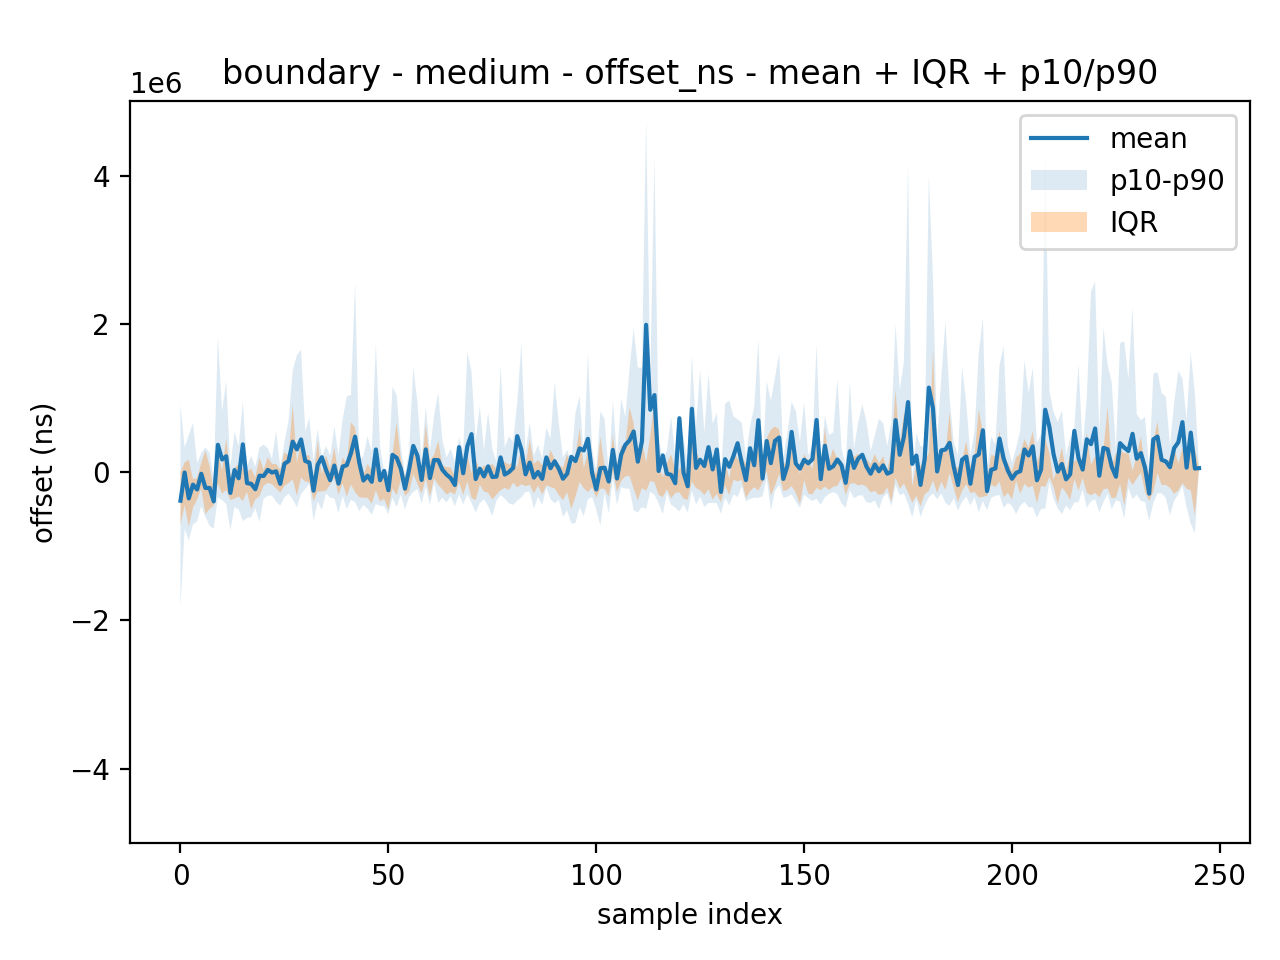
\includegraphics[width=\linewidth]{
      pars_plots/ptp/_aggregated/boundary/medium/offset_ns_mean_iqr_p10_p90.png
    }
    \caption{Scenario MEDIUM}
  \end{subfigure}
  \begin{subfigure}
    {0.32\textwidth}
    \centering
    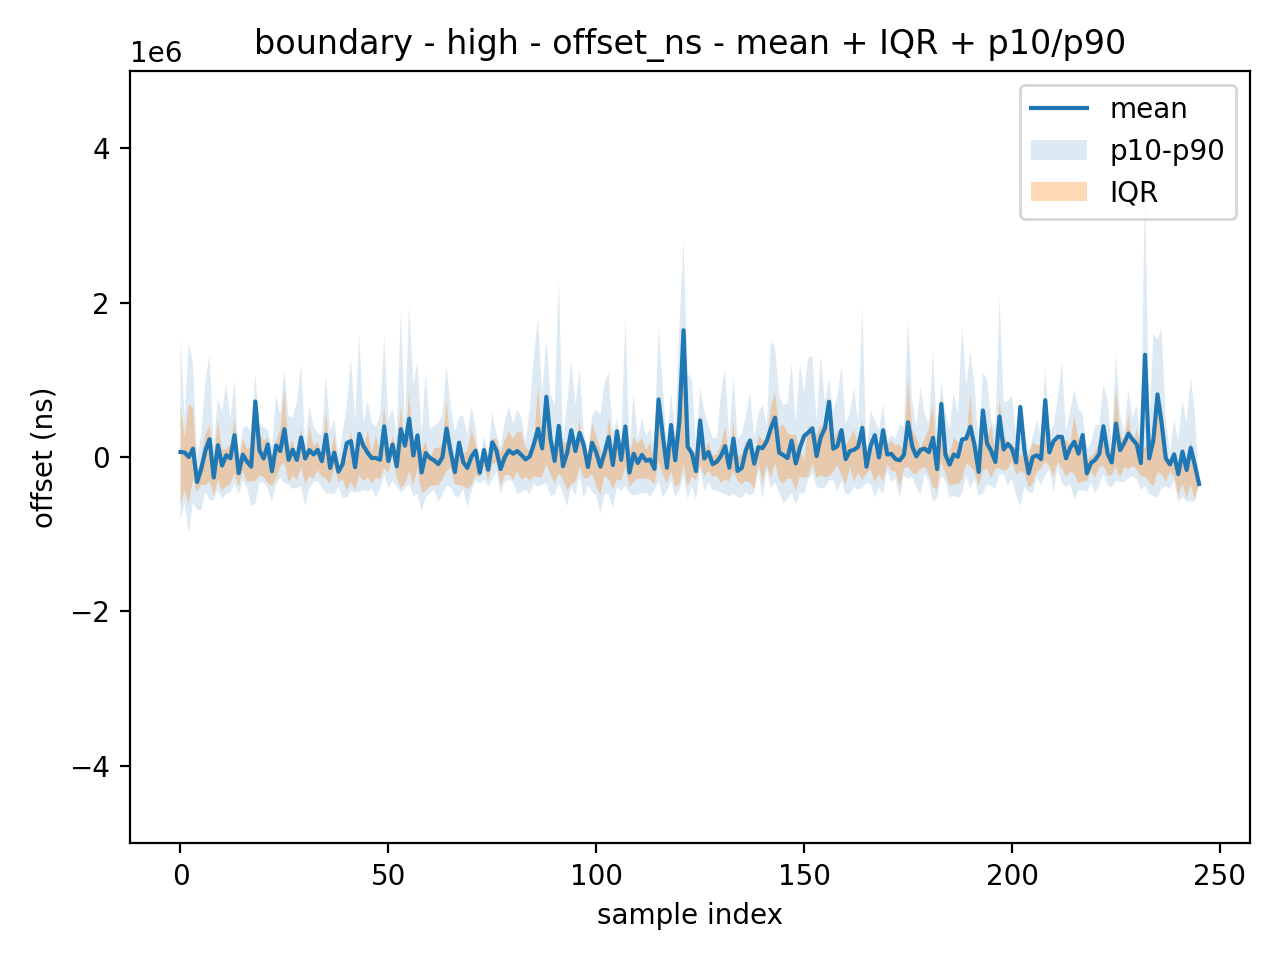
\includegraphics[width=\linewidth]{
      pars_plots/ptp/_aggregated/boundary/high/offset_ns_mean_iqr_p10_p90.png
    }
    \caption{Scenario HIGH}
  \end{subfigure}
  \caption{Media con banda inter-quartile e banda p10-p90 - nodo: \texttt{boundary}}
  \label{fig:scenario_comparison}
\end{figure}

Anche i dati dell'\texttt{offset} confermano il trend. I tre scenari evidenziano un
andamento complessivamente centrato in prossimità dello zero, con oscillazioni
di segno alterno e picchi sporadici.

Il valore medio dell'\texttt{offset} è di ~87.809~\textmu s nello scenario
\texttt{low}, ~153.961~\textmu s nello scenario \texttt{medium} e ~110.782~\textmu
s nello scenario \texttt{high}. La mediana assume valori contenuti rispettivamente
nei tre scenari,con valori di ~45.375~\textmu s, ~97.301~\textmu s e ~65.087~\textmu
s. I risultati mostrano una lieve prevalenza di offset positivo, ma sempre compatibile
con le premesse.

L'ampiezza inter-quartile media è di ~279.114~\textmu s nello scenario \texttt{low},
~327.530~\textmu s nello scenario \texttt{medium} e ~250.843~\textmu s nello scenario
\texttt{high}. La banda p10--p90 media assume valori pari a circa 1017.673~\textmu
s, 1243.040~\textmu s e 1122.148~\textmu s. L'osservazione dei profili temporali
porta alle stesse conclusioni.

Nel complesso, l'\texttt{offset} del \texttt{boundary} conferma una condizione di
stabilità della sincronizzazione. Le differenze osservate tra i tre scenari
appaiono limitate, non monotone e non sufficienti a sostenere l'ipotesi di un impatto
diretto del degrado downstream sulla sincronizzazione del \texttt{boundary}
rispetto al \texttt{servergm}.

\section{\texttt{chronyd}}
Per quanto riguarda il demone \texttt{Chrony}, l'analisi è stata svolta su una topologia
composta dal solo collegamento tra \texttt{servergm} e \texttt{clientchrony}. In
questo contesto, il degrado di rete tramite \texttt{tc}/\texttt{netem} è stato applicato
in due configurazioni distinte: in un primo caso sull'interfaccia del \texttt{clientchrony},
in un secondo caso sull'interfaccia del \texttt{servergm}.

La doppia configurazione permette di osservare in modo separato effetti del degrado
introdotto lungo le due direzioni logiche della comunicazione tra client e server.

Nei risultati proposti, quindi, oltre alla comparazione dei differenti scenari,
si ha la distinzione delle due configurazioni.È utile precisare che tutte le
metriche analizzate sono state rilevate esclusivamente tramite interrogazione
del nodo \texttt{clientchrony}, poiché è da esso che si ricavano le misure
direttamente rilevanti per valutare la qualità della sincronizzazione dal punto
di vista del client.

\subsection{Analisi metrica: \texttt{offset}}
\begin{figure}[H]
  \centering

  \begin{subfigure}
    {0.32\textwidth}
    \centering
    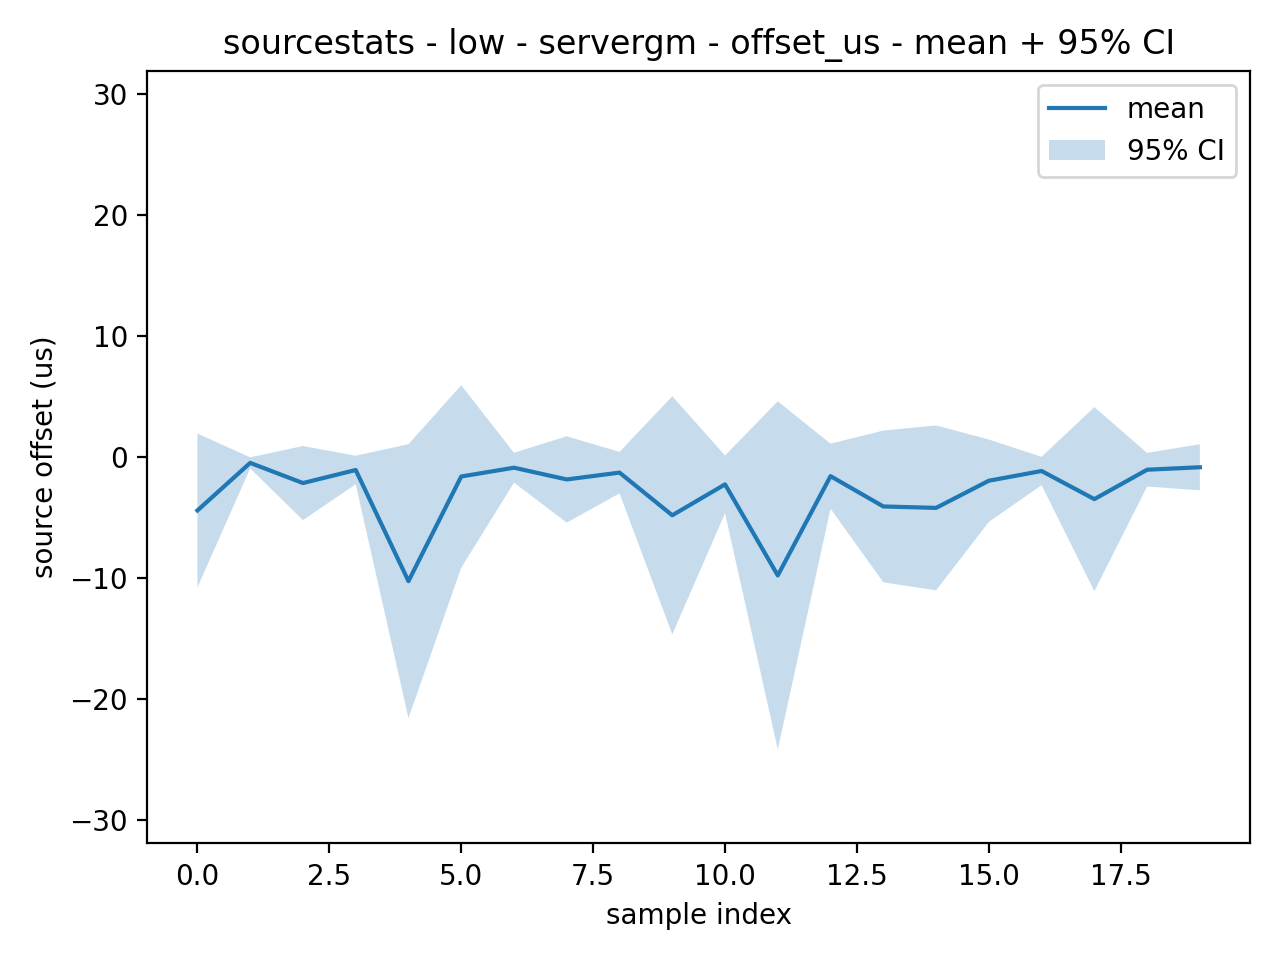
\includegraphics[width=\linewidth]{
      pars_plots/chrony_clientchrony/_aggregated/sourcestats/low/servergm/offset_us_mean_ci95.png
    }
    \caption{Scenario LOW}
  \end{subfigure}
  \hfill
  \begin{subfigure}
    {0.32\textwidth}
    \centering
    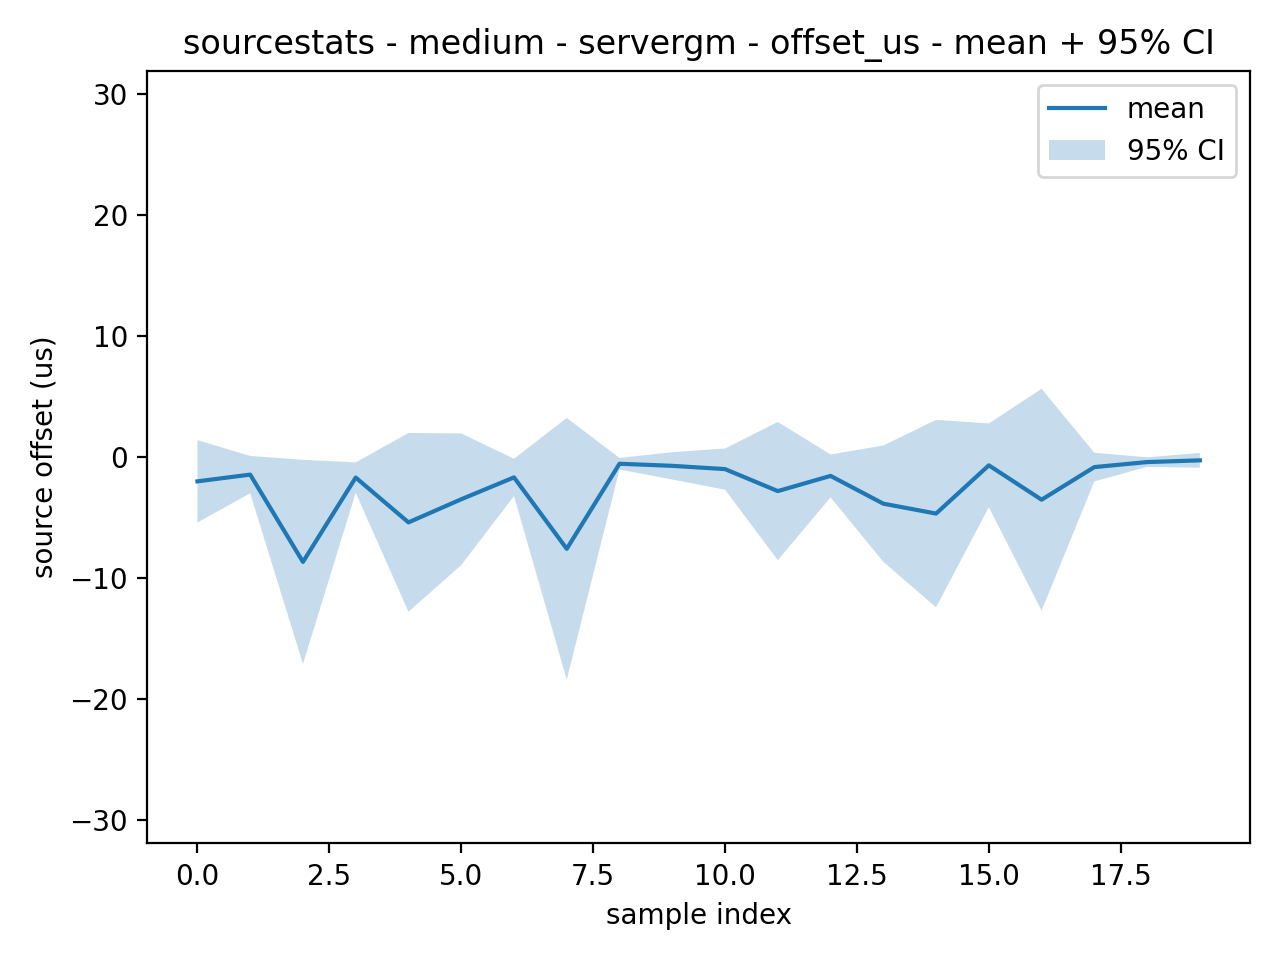
\includegraphics[width=\linewidth]{
      pars_plots/chrony_clientchrony/_aggregated/sourcestats/medium/servergm/offset_us_mean_ci95.png
    }
    \caption{Scenario MEDIUM}
  \end{subfigure}
  \begin{subfigure}
    {0.32\textwidth}
    \centering
    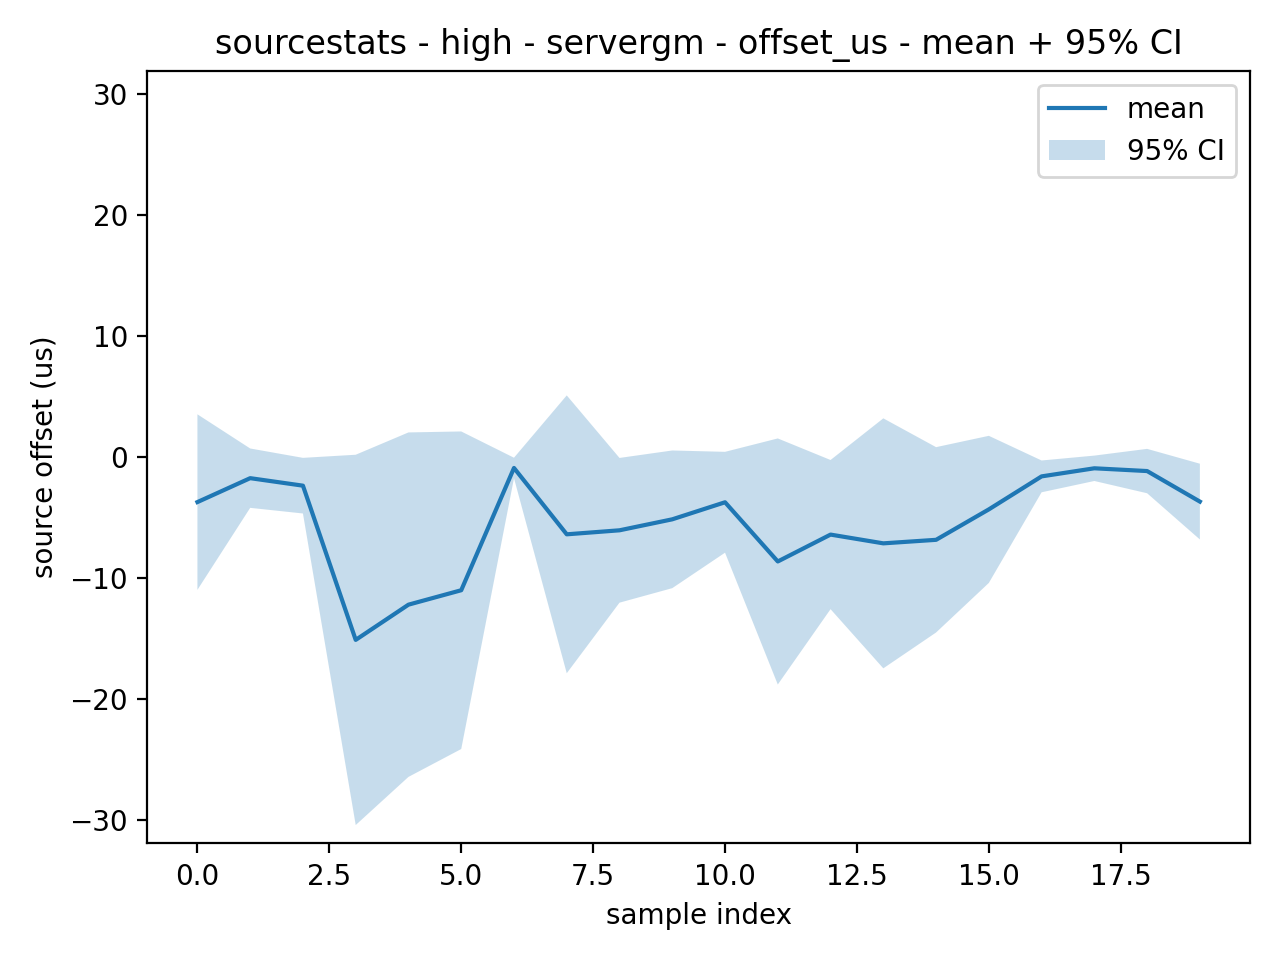
\includegraphics[width=\linewidth]{
      pars_plots/chrony_clientchrony/_aggregated/sourcestats/high/servergm/offset_us_mean_ci95.png
    }
    \caption{Scenario HIGH}
  \end{subfigure}
  \caption{Media con intervallo di confidenza al 95\% - nodo: \texttt{clientchrony}
  - netem/tc: \texttt{clientchrony}}
  \label{fig:scenario_comparison}
\end{figure}
\begin{figure}[H]
  \centering

  \begin{subfigure}
    {0.32\textwidth}
    \centering
    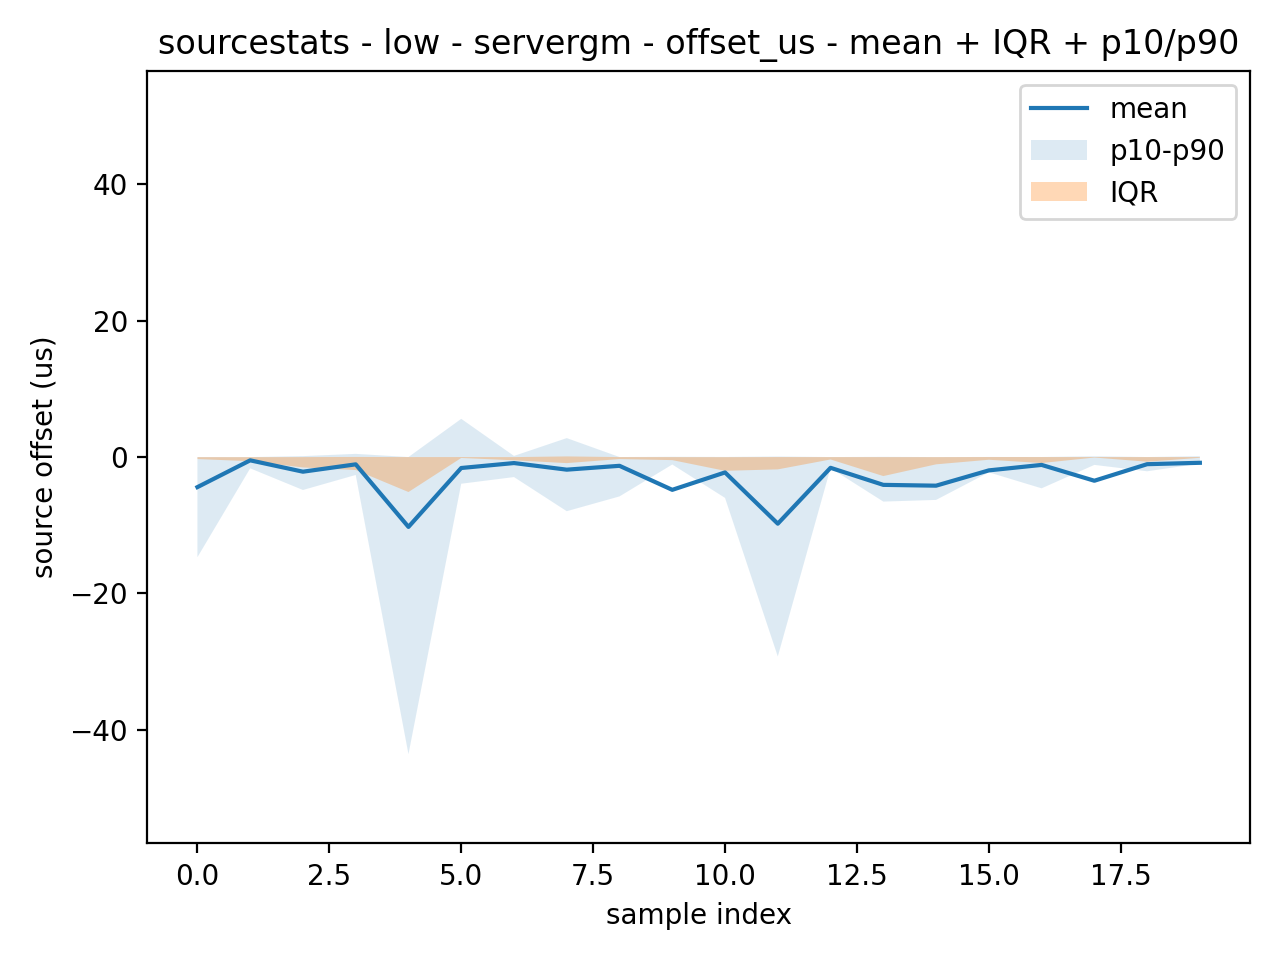
\includegraphics[width=\linewidth]{
      pars_plots/chrony_clientchrony/_aggregated/sourcestats/low/servergm/offset_us_mean_iqr_p10_p90.png
    }
    \caption{Scenario LOW}
  \end{subfigure}
  \hfill
  \begin{subfigure}
    {0.32\textwidth}
    \centering
    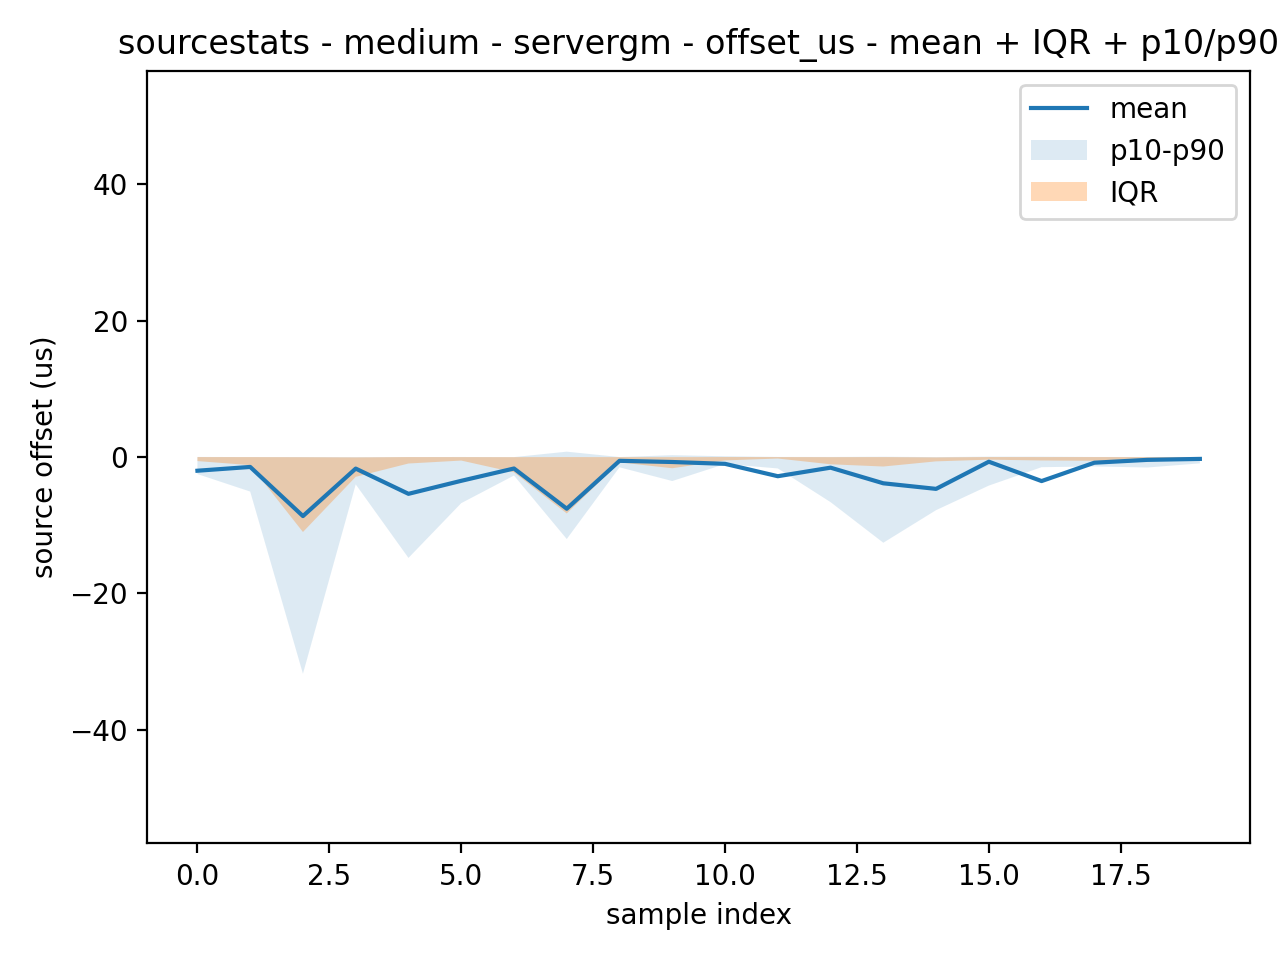
\includegraphics[width=\linewidth]{
      pars_plots/chrony_clientchrony/_aggregated/sourcestats/medium/servergm/offset_us_mean_iqr_p10_p90.png
    }
    \caption{Scenario MEDIUM}
  \end{subfigure}
  \begin{subfigure}
    {0.32\textwidth}
    \centering
    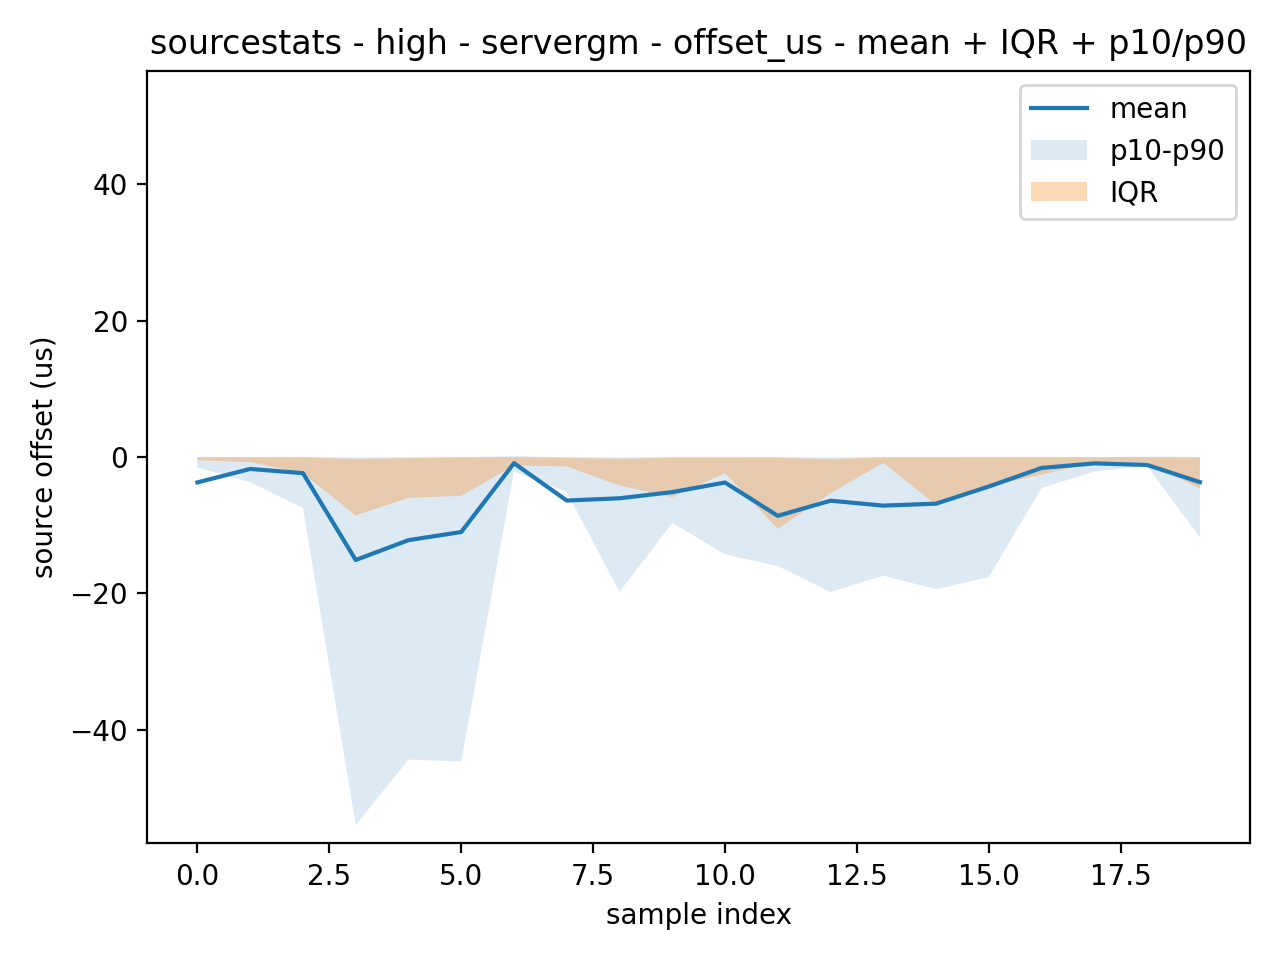
\includegraphics[width=\linewidth]{
      pars_plots/chrony_clientchrony/_aggregated/sourcestats/high/servergm/offset_us_mean_iqr_p10_p90.png
    }
    \caption{Scenario HIGH}
  \end{subfigure}
  \caption{Media con banda inter-quartile e banda p10-p90 - nodo: \texttt{clientchrony}
  - netem/tc: \texttt{clientchrony}}
  \label{fig:scenario_comparison}
\end{figure}
\paragraph*{clientchrony - netem/tc:}
Nel caso della metrica \texttt{offset\_us}, l'analisi relativa a \texttt{clientchrony}
vi è un peggioramento progressivo all'aumentare dell'intensità dello scenario, nonostante
non venga compromessa la sincronizzazione verso la sorgente.

Nel caso \texttt{low}, si ha una curva delle medie vicino all zero, ma con
prevalenza di valori leggermente negativi. L'aggregazione sulle curve fornisce una
media di ~\texttt{-2.958 \,$\mu$s} e i valori medi sono compresi nell'intervallo ~\texttt{-10.250
\,$\mu$s} e ~\texttt{-0.481 \,$\mu$s}. Per quanto riguarda le statistiche
globali sui campioni si ha la mediana pari a ~\texttt{-0.049 \,$\mu$s}, il primo quartile
è ~\texttt{-0.927 \,$\mu$s} e il terzo quartile è ~\texttt{-0.002 \,$\mu$s}. L'ampiezza
media dell'intervallo ~\texttt{p10-p90}, pari a ~\texttt{7.971 \,$\mu$s}. La
banda inter-quartile media è contenuta, con un valore di ~\texttt{1.095 \,$\mu$s}.
In questo scenario il degrado introdotto sul client produce soltanto un lieve
sbilanciamento negativo dell'offset, senza alterare in modo significativo il regime
di sincronizzazione.

Nel caso \texttt{medium} cresce la dispersione e compaiono fluttuazioni negative
più frequenti. La media della curva aggregata è pari a \texttt{-2.642 \,$\mu$s}, simile
al caso \texttt{low}, ma i grafici evidenziano dei picchi più accentuati. La
mediana è ~\texttt{-0.073 \,$\mu$s}, il primo quartile ~\texttt{-1.075 \,$\mu$s} e
il terzo quartile ~\texttt{-0.004 \,$\mu$s}. Il peggioramento è principalmente
evidente nella variabilità. L'ampiezza media della banda \texttt{p10-p90} è di ~\texttt{6.266
\,$\mu$s}. La banda inter-quartile media cresce a \texttt{1.804 \,$\mu$s}.Inoltre,
il valore massimo dell'IQR raggiunge \texttt{10.978 \,$\mu$s}, segnale che in
alcuni punti il comportamento tra le run diventa più irregolare.

Nello scenario \texttt{high}, la media delle curve aggregate scende a \texttt{-5.451
\,$\mu$s}, quindi circa il doppio in valore assoluto rispetto ai casi \texttt{low}
e \texttt{medium}, e la curva delle medie mostra tratti più chiaramente distanti dallo
zero, con minimi fino a \texttt{-15.103 \,$\mu$s}. La mediana resta vicino allo
zero (\texttt{-0.360 \,$\mu$s}). Non c'è quindi un peggioramento uniforme su
tutti i campioni. Vi è un aumento della dispersione. L'ampiezza media dell'intervallo
\texttt{p10-p90} è di ~\texttt{15.836 \,$\mu$s}, e l'IQR medio è di ~\texttt{3.693
\,$\mu$s}.

In tutti e tre gli scenari, in molteplici punti, la curva media è esterna alla banda inter-quartile.
Quindi si ha un valore medio non coincidente con il comportamento tipico della run, risentendo maggiormente
di anomalie o di code negative della distribuzione.

Nei primi due casi i risultati sono sufficientemente uniformi, mentre nello scenario
\texttt{high} vi è un peggioramento più marcato.

\begin{figure}[H]
  \centering

  \begin{subfigure}
    {0.32\textwidth}
    \centering
    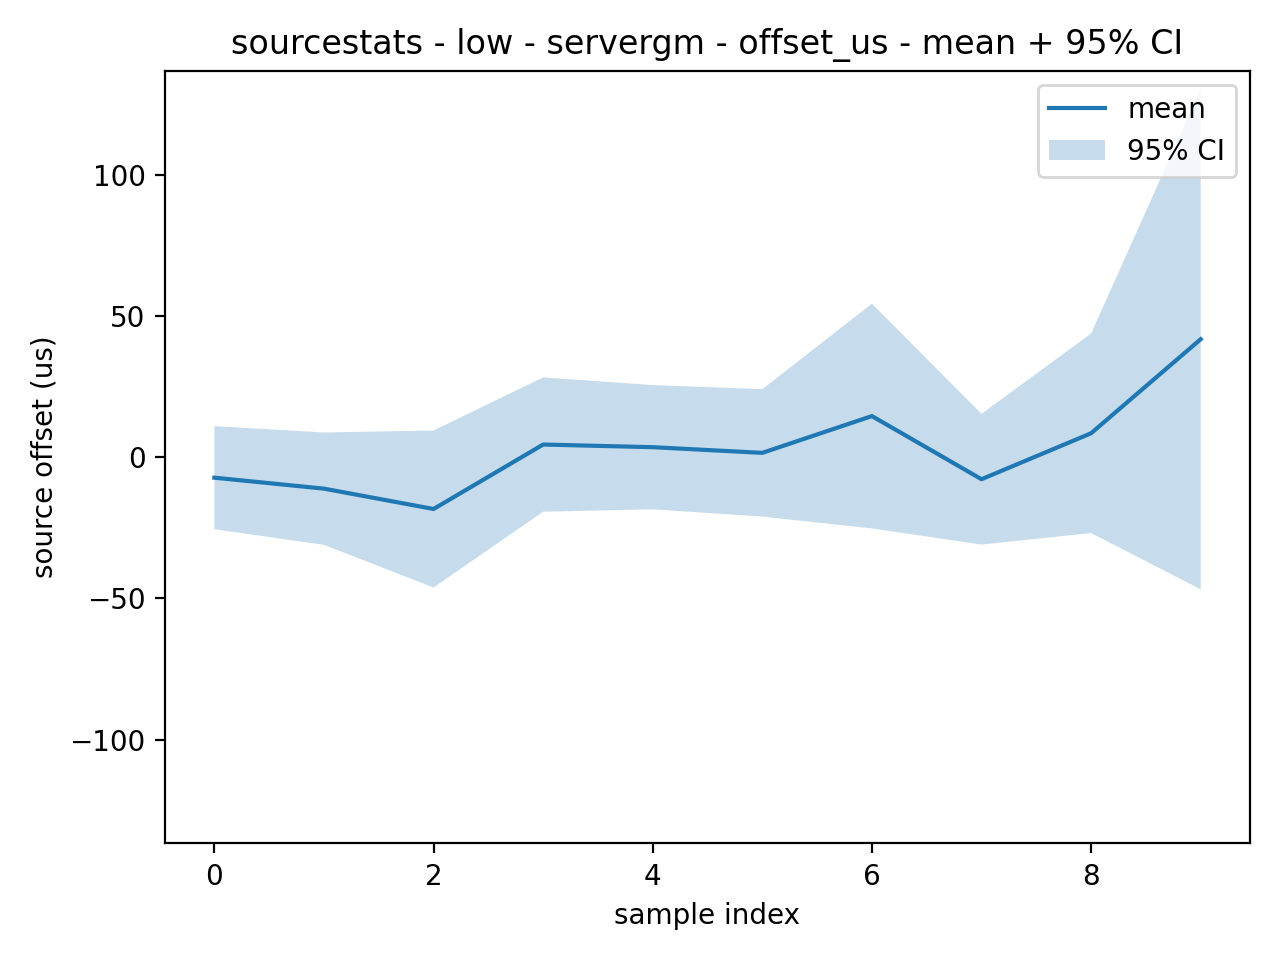
\includegraphics[width=\linewidth]{
      pars_plots/chrony_servergm/_aggregated/sourcestats/low/servergm/offset_us_mean_ci95.png
    }
    \caption{Scenario LOW}
  \end{subfigure}
  \hfill
  \begin{subfigure}
    {0.32\textwidth}
    \centering
    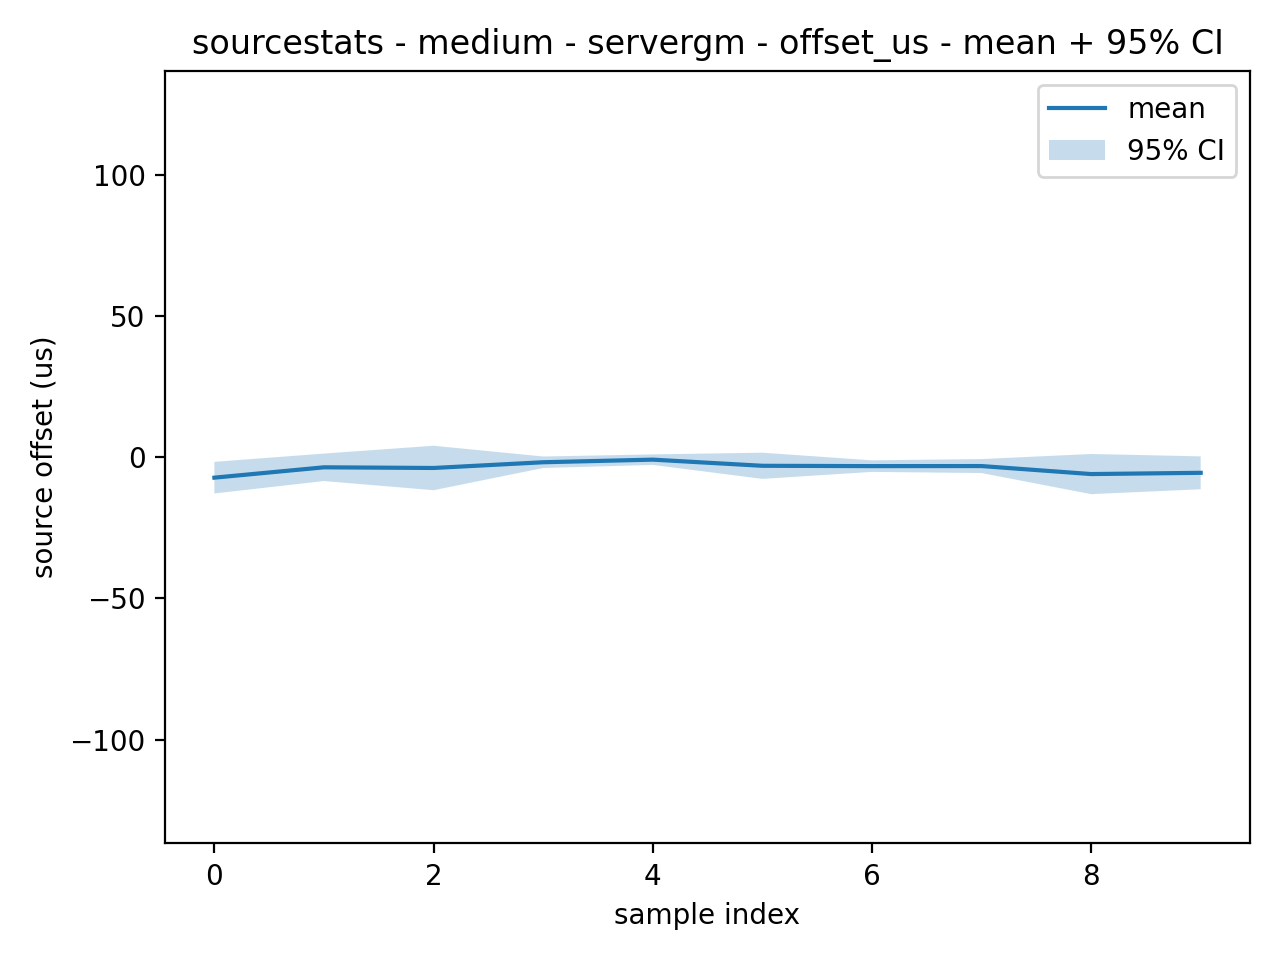
\includegraphics[width=\linewidth]{
      pars_plots/chrony_servergm/_aggregated/sourcestats/medium/servergm/offset_us_mean_ci95.png
    }
    \caption{Scenario MEDIUM}
  \end{subfigure}
  \begin{subfigure}
    {0.32\textwidth}
    \centering
    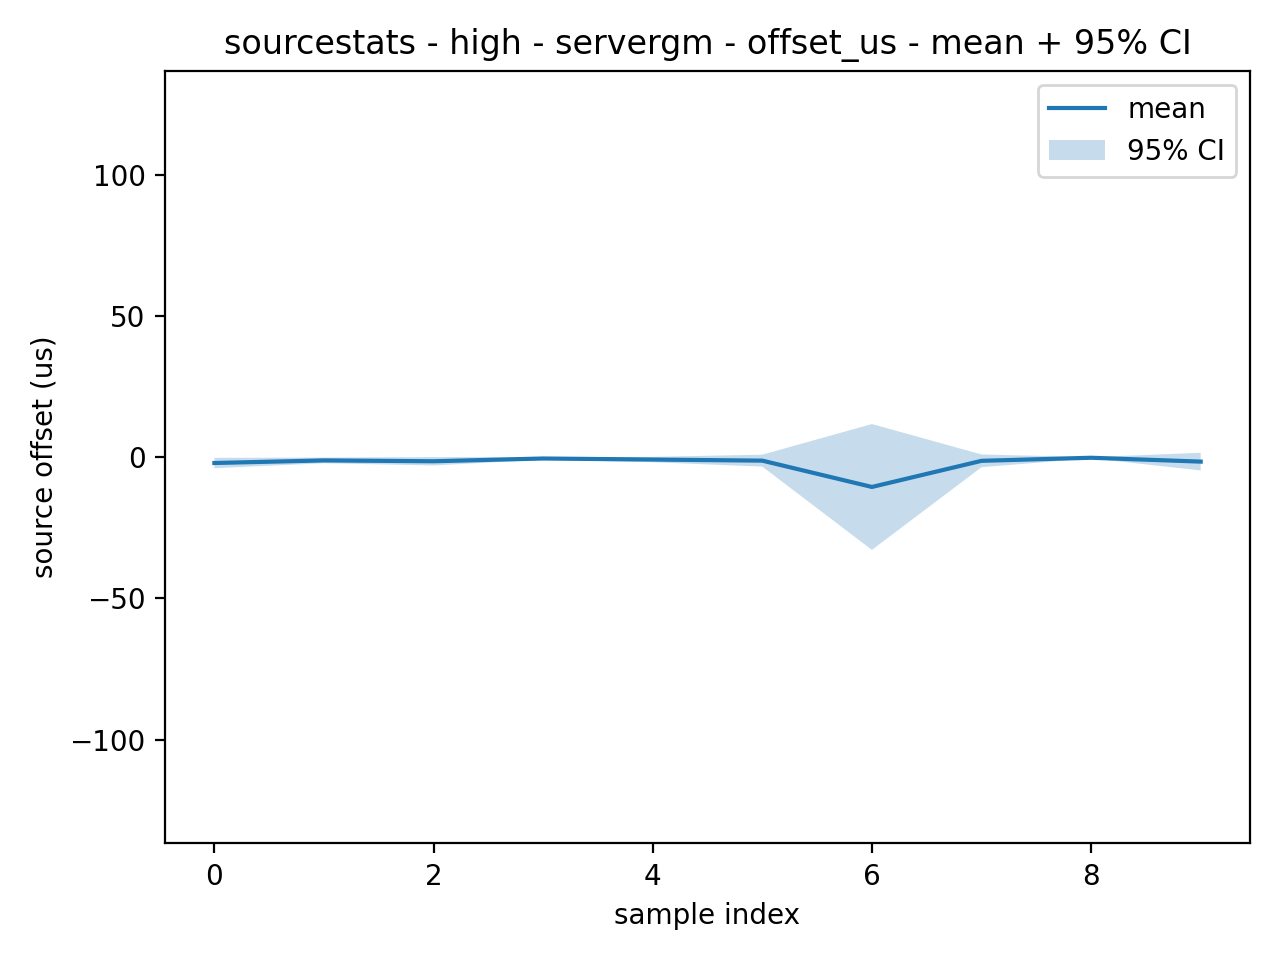
\includegraphics[width=\linewidth]{
      pars_plots/chrony_servergm/_aggregated/sourcestats/high/servergm/offset_us_mean_ci95.png
    }
    \caption{Scenario HIGH}
  \end{subfigure}
  \caption{Media con intervallo di confidenza al 95\% - nodo: \texttt{clientchrony}
  - netem/tc: \texttt{servergm}}
  \label{fig:scenario_comparison}
\end{figure}
\begin{figure}[H]
  \centering

  \begin{subfigure}
    {0.32\textwidth}
    \centering
    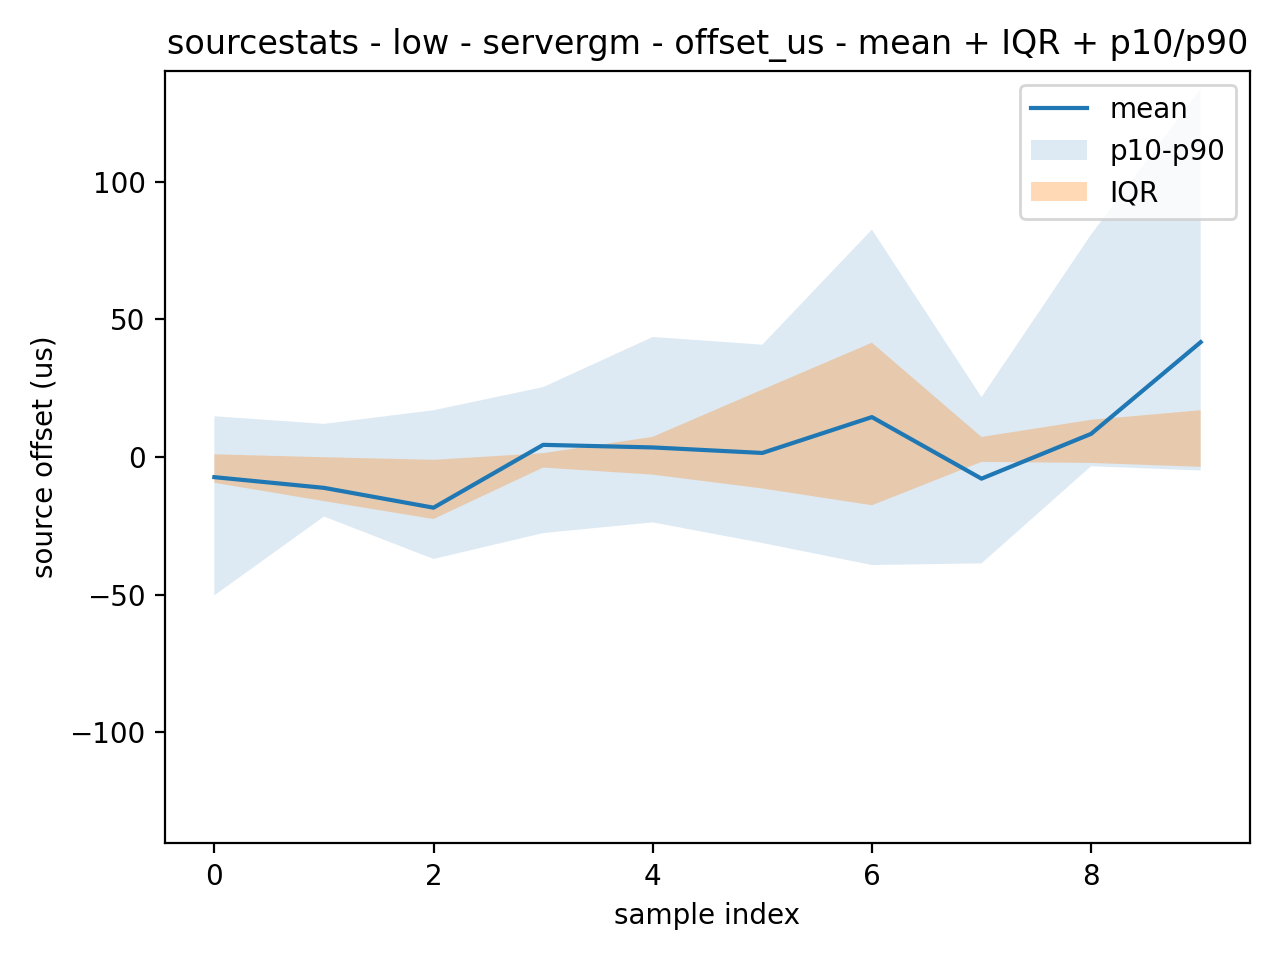
\includegraphics[width=\linewidth]{
      pars_plots/chrony_servergm/_aggregated/sourcestats/low/servergm/offset_us_mean_iqr_p10_p90.png
    }
    \caption{Scenario LOW}
  \end{subfigure}
  \hfill
  \begin{subfigure}
    {0.32\textwidth}
    \centering
    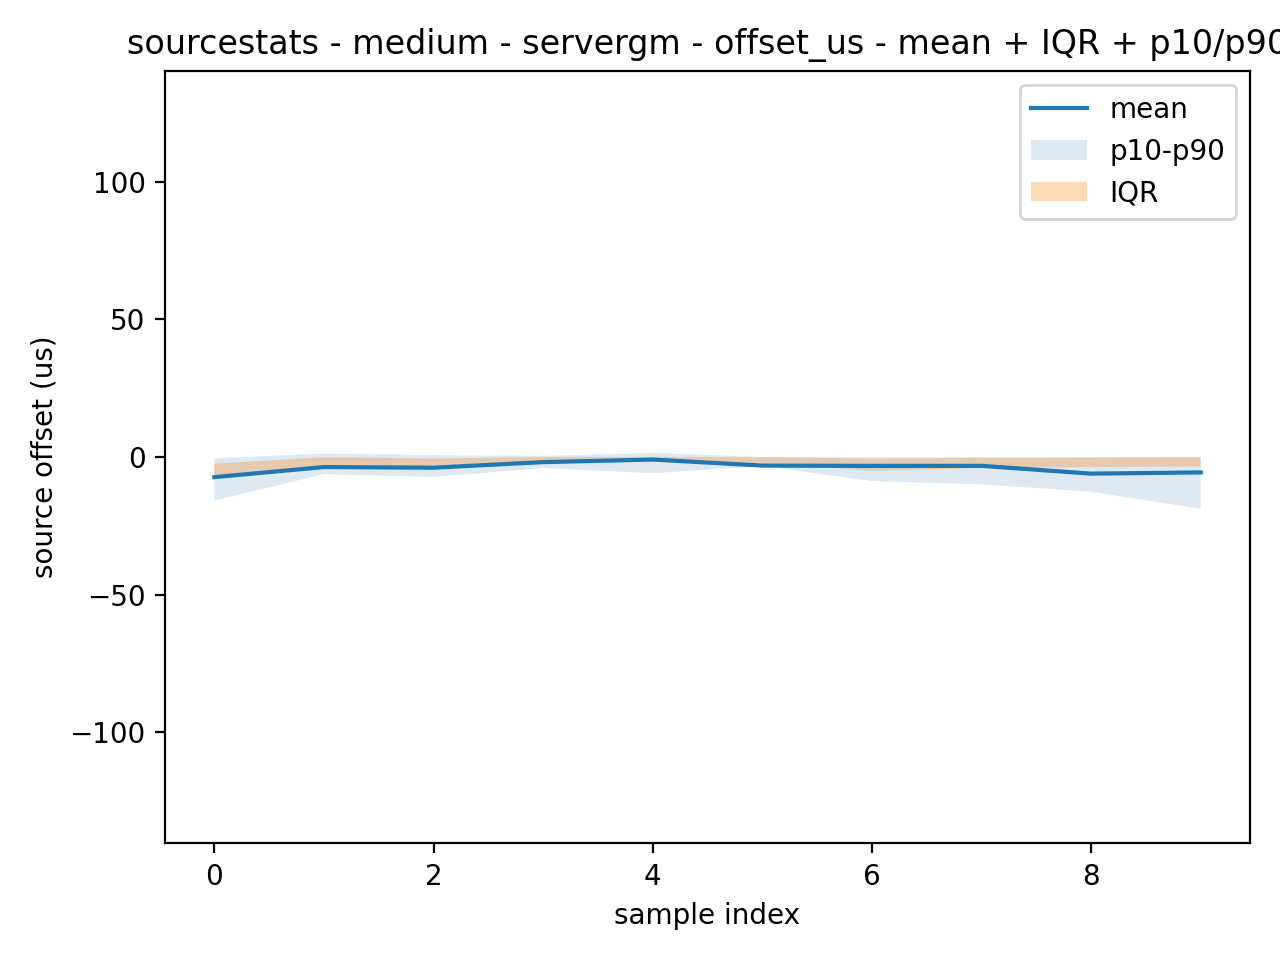
\includegraphics[width=\linewidth]{
      pars_plots/chrony_servergm/_aggregated/sourcestats/medium/servergm/offset_us_mean_iqr_p10_p90.png
    }
    \caption{Scenario MEDIUM}
  \end{subfigure}
  \begin{subfigure}
    {0.32\textwidth}
    \centering
    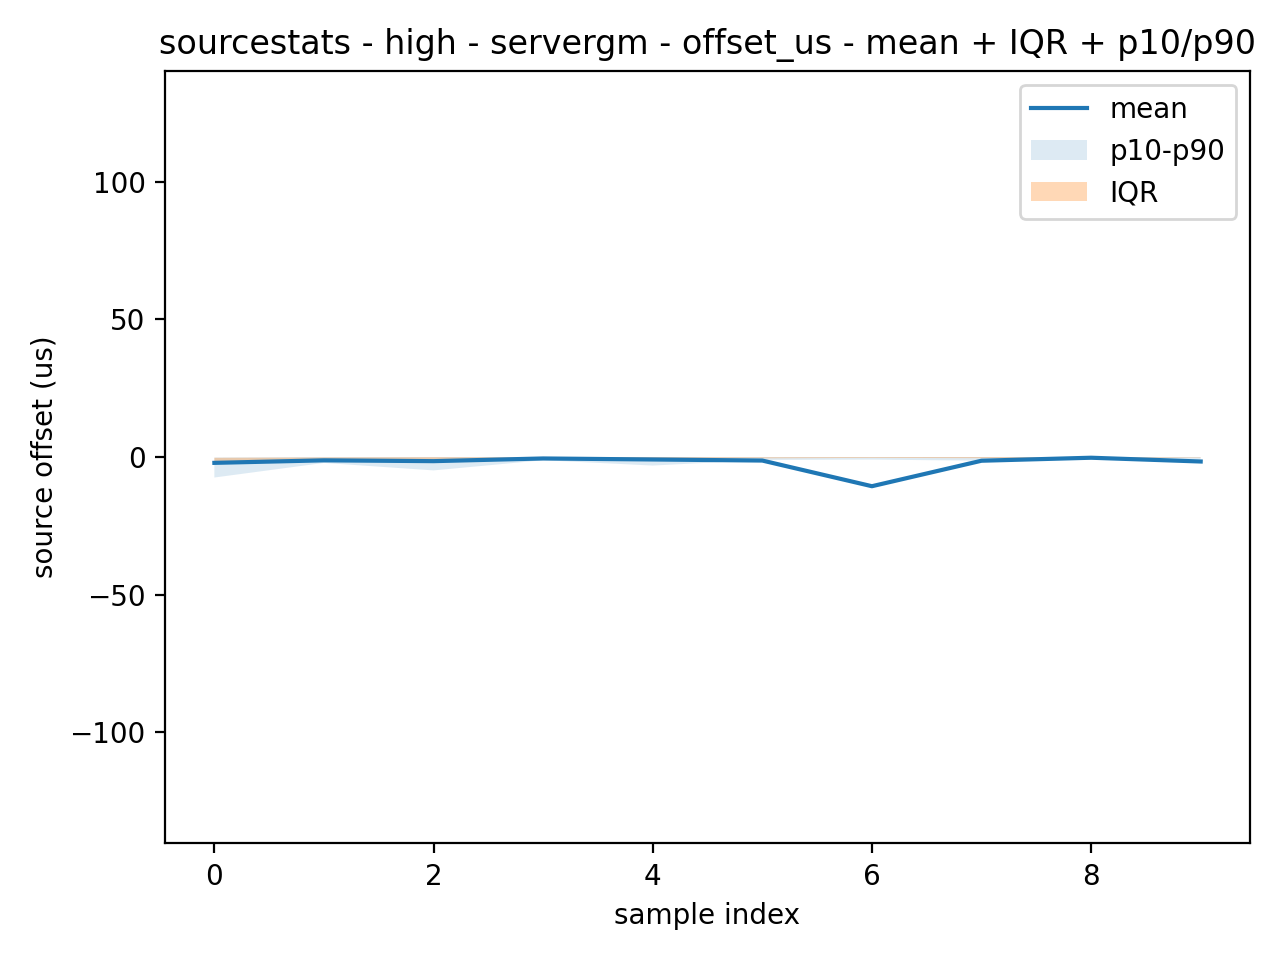
\includegraphics[width=\linewidth]{
      pars_plots/chrony_servergm/_aggregated/sourcestats/high/servergm/offset_us_mean_iqr_p10_p90.png
    }
    \caption{Scenario HIGH}
  \end{subfigure}
  \caption{Media con banda inter-quartile e banda p10-p90 - nodo: \texttt{clientchrony}
  - netem/tc: \texttt{servergm}}
  \label{fig:scenario_comparison}
\end{figure}
\paragraph*{servergm - netem/tc:}
La \texttt{offset\_us} riferita alla sezione \texttt{sourcestats}, l'evidenzia
un comportamento non monotono al variare dello scenario, ma nel complesso compatibile
con una sincronizzazione che resta attiva e generalmente prossima alla sorgente di
riferimento.

Nello scenario \texttt{low}. Il valor medio è di ~\texttt{2.935 \,$\mu$s},
prossimo allo zero, La deviazione standard delle medie è \texttt{16.824 \,$\mu$s},
con valori in un intervallo di \texttt{-18.383 \,$\mu$s} e \texttt{41.717 \,$\mu$s}.
Le bande di variabilità sono ampie, con una larghezza media dell'intervallo \texttt{p10-p90}
pari a \texttt{74.976 \,$\mu$s} con presenza di picchi fino a \texttt{138.489 \,$\mu$s}.
Il comportamento nello scenario \texttt{low} è caratterizzato da variabilità
inter-run e da outlier positivi che ampliano sensibilmente la dispersione
osservata.

Nel caso \texttt{medium}, c'è un comportamento più regolare. Si ha una media aggregata
di ~\texttt{-3.863 \,$\mu$s}. La dispersione è ridotta notevolmente la deviazione
standard delle medie scende a \texttt{1.935 \,$\mu$s}, mentre l'intervallo medio
\texttt{p10-p90} è di ~\texttt{9.546 \,$\mu$s}.In questo caso l'offset contenuto vicino
allo zero e mostra una variabilità minore rispetto al caso precedente.

Nello scenario \texttt{high} si ha un comportamento stabile. La media aggregata della
curva è pari a \texttt{-2.122 \,$\mu$s}. La deviazione standard delle medie è \texttt{3.022
\,$\mu$s}. L'ampiezza media dell'IQR è di ~\texttt{0.709 \,$\mu$s}, mentre l'intervallo
medio \texttt{p10-p90} è pari a \texttt{2.355 \,$\mu$s}, valori che descrivono una
forte concentrazione della parte centrale della distribuzione. Nel grafico è
visibile una singola flessione più marcata, coerente con il minimo della curva pari
a \texttt{-10.588 \,$\mu$s}.

Nel confronto complessivo non c'è un risultato lineare. Il caso \texttt{low}
mostra maggiore dispersione con valori anomali, mantenendo comunque valori prossimi
allo zero. I casi \texttt{medium} e \texttt{high} appaiono invece più regolari. Tale
metrica non produce una deriva sistematica progressivamente crescente al variare dello
scenario.

\paragraph*{Confronto:}
L'impairment introdotto su \texttt{clientchrony} si hanno valori sulla metrica più
coerenti: al crescere dello scenario si osserva un progressivo peggioramento, con
medie che si spostano verso valori più negativi e con un aumento della dispersione. Nel
caso invece di \texttt{servergm}, il comportamento appare meno regolare e non monotono.
In sintesi, applicando il degrado sul lato client si manifestano dati più coerenti
con le aspettative.

\subsection{Analisi metrica: \texttt{stddev}}
\begin{figure}[H]
  \centering

  \begin{subfigure}
    {0.32\textwidth}
    \centering
    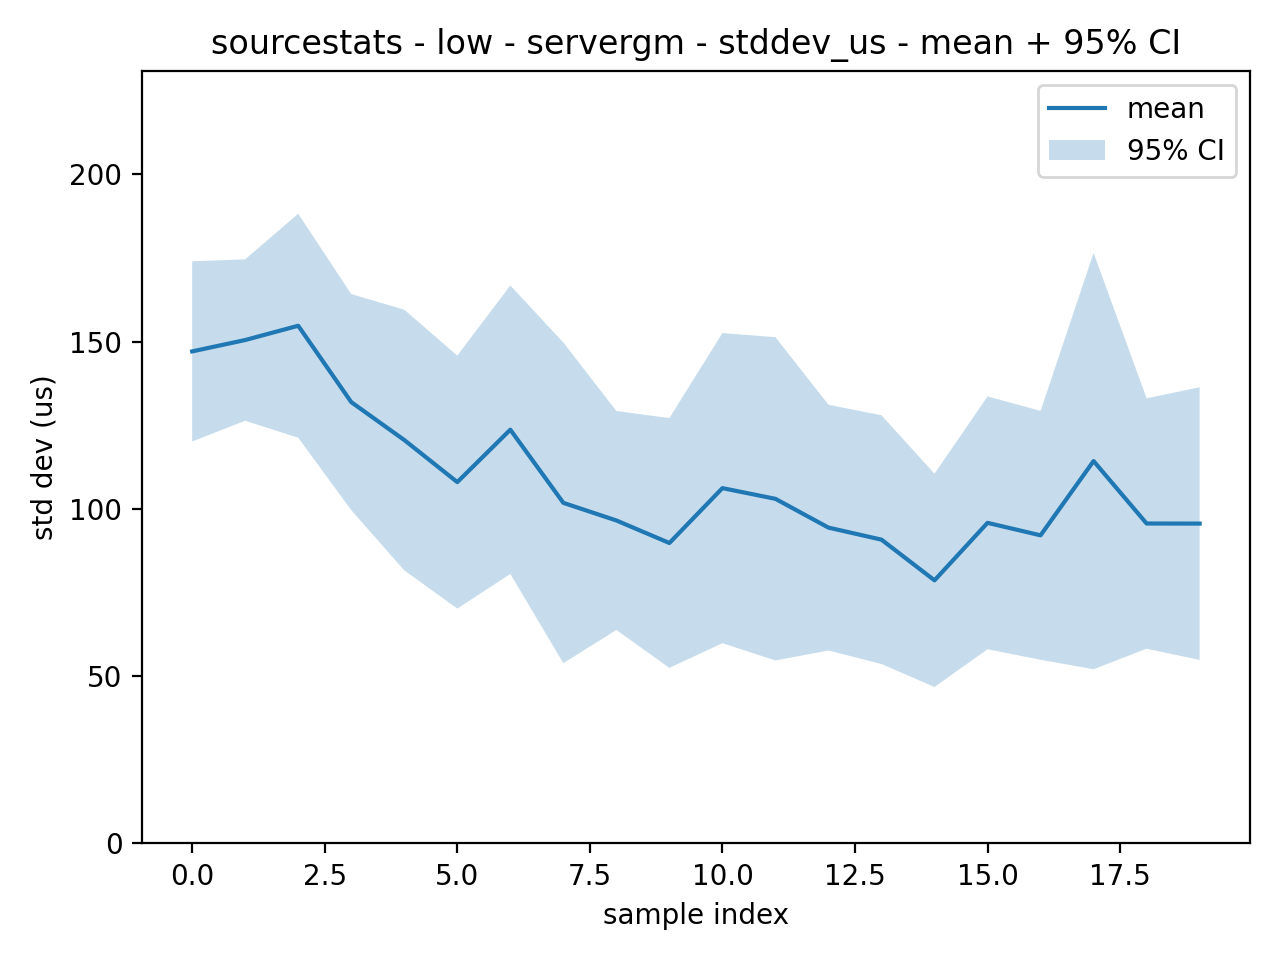
\includegraphics[width=\linewidth]{
      pars_plots/chrony_clientchrony/_aggregated/sourcestats/low/servergm/stddev_us_mean_ci95.png
    }
    \caption{Scenario LOW}
  \end{subfigure}
  \hfill
  \begin{subfigure}
    {0.32\textwidth}
    \centering
    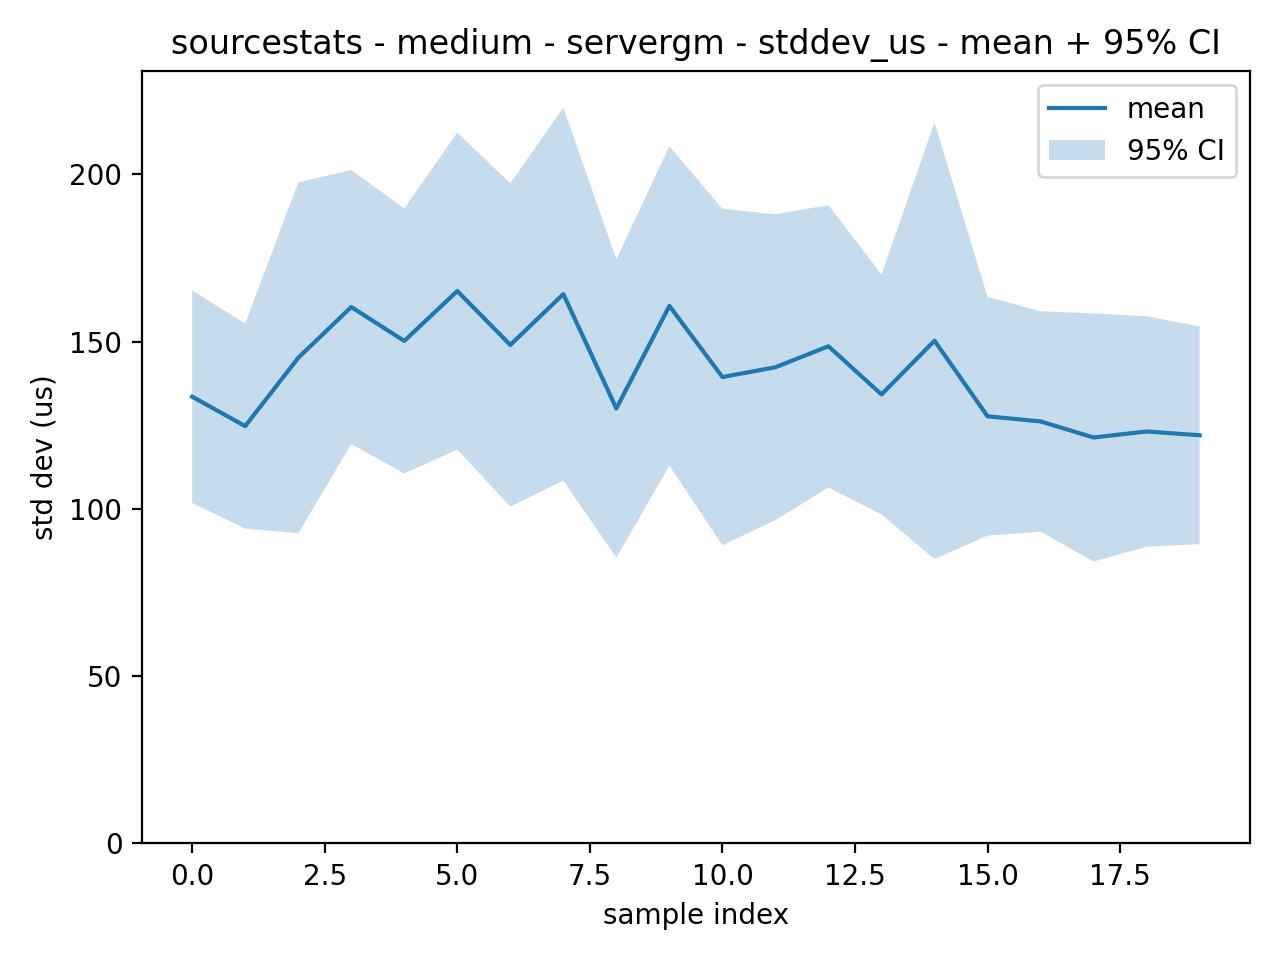
\includegraphics[width=\linewidth]{
      pars_plots/chrony_clientchrony/_aggregated/sourcestats/medium/servergm/stddev_us_mean_ci95.png
    }
    \caption{Scenario MEDIUM}
  \end{subfigure}
  \begin{subfigure}
    {0.32\textwidth}
    \centering
    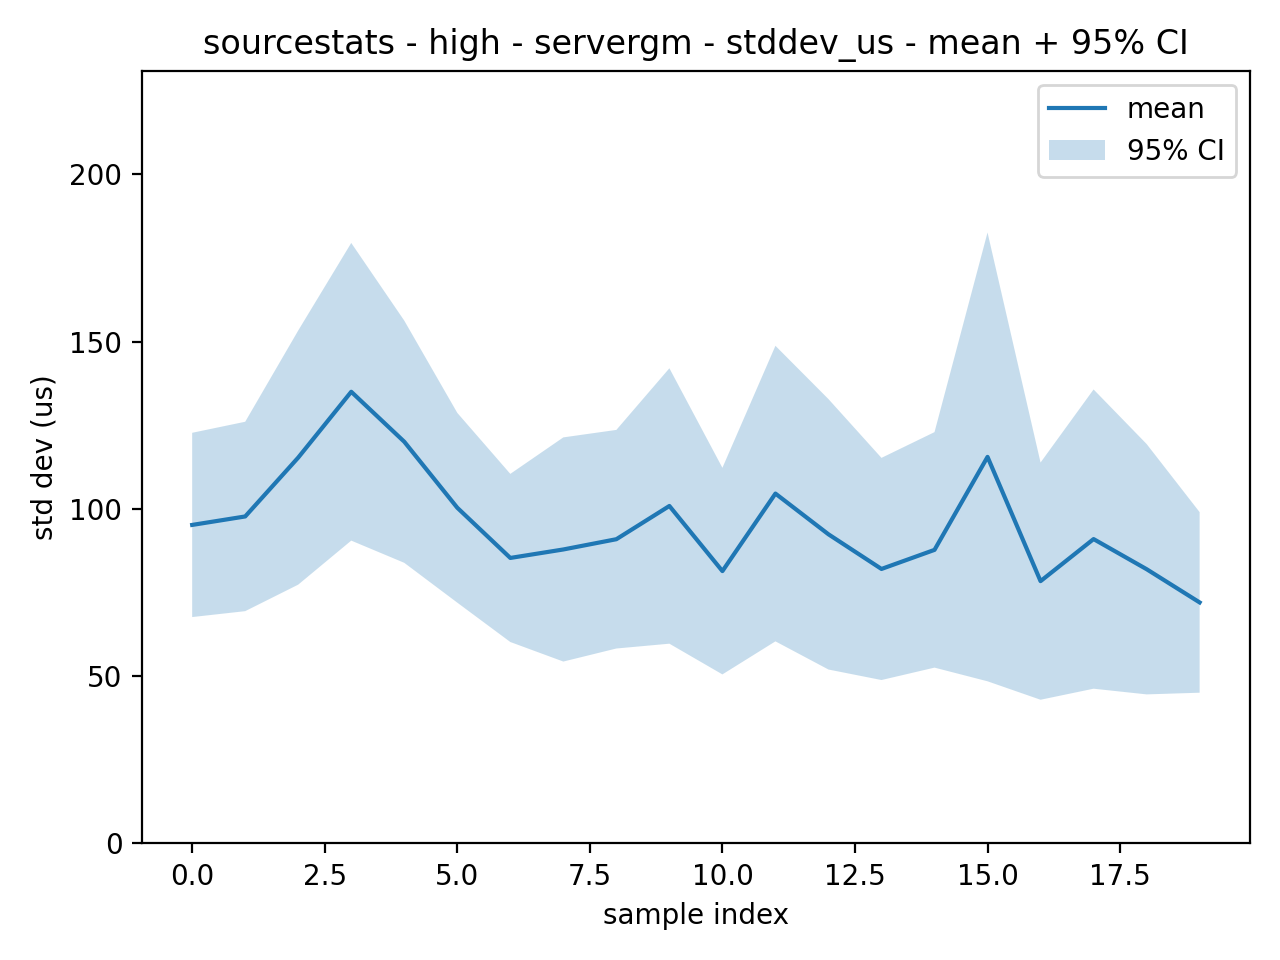
\includegraphics[width=\linewidth]{
      pars_plots/chrony_clientchrony/_aggregated/sourcestats/high/servergm/stddev_us_mean_ci95.png
    }
    \caption{Scenario HIGH}
  \end{subfigure}
  \caption{Media con intervallo di confidenza al 95\% - nodo: \texttt{clientchrony}
  - netem/tc: \texttt{clientchrony}}
  \label{fig:scenario_comparison}
\end{figure}
\begin{figure}[H]
  \centering

  \begin{subfigure}
    {0.32\textwidth}
    \centering
    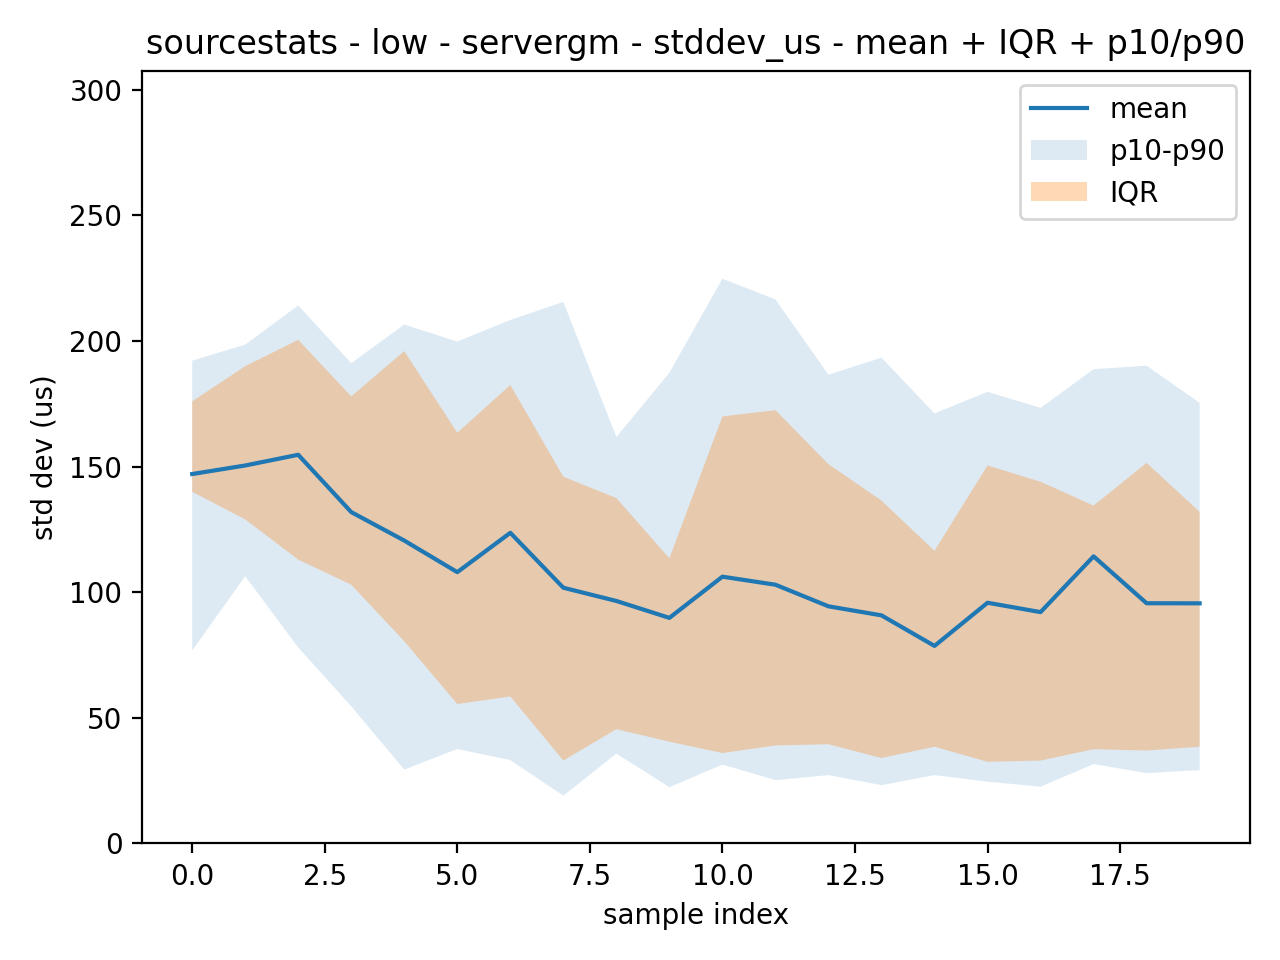
\includegraphics[width=\linewidth]{
      pars_plots/chrony_clientchrony/_aggregated/sourcestats/low/servergm/stddev_us_mean_iqr_p10_p90.png
    }
    \caption{Scenario LOW}
  \end{subfigure}
  \hfill
  \begin{subfigure}
    {0.32\textwidth}
    \centering
    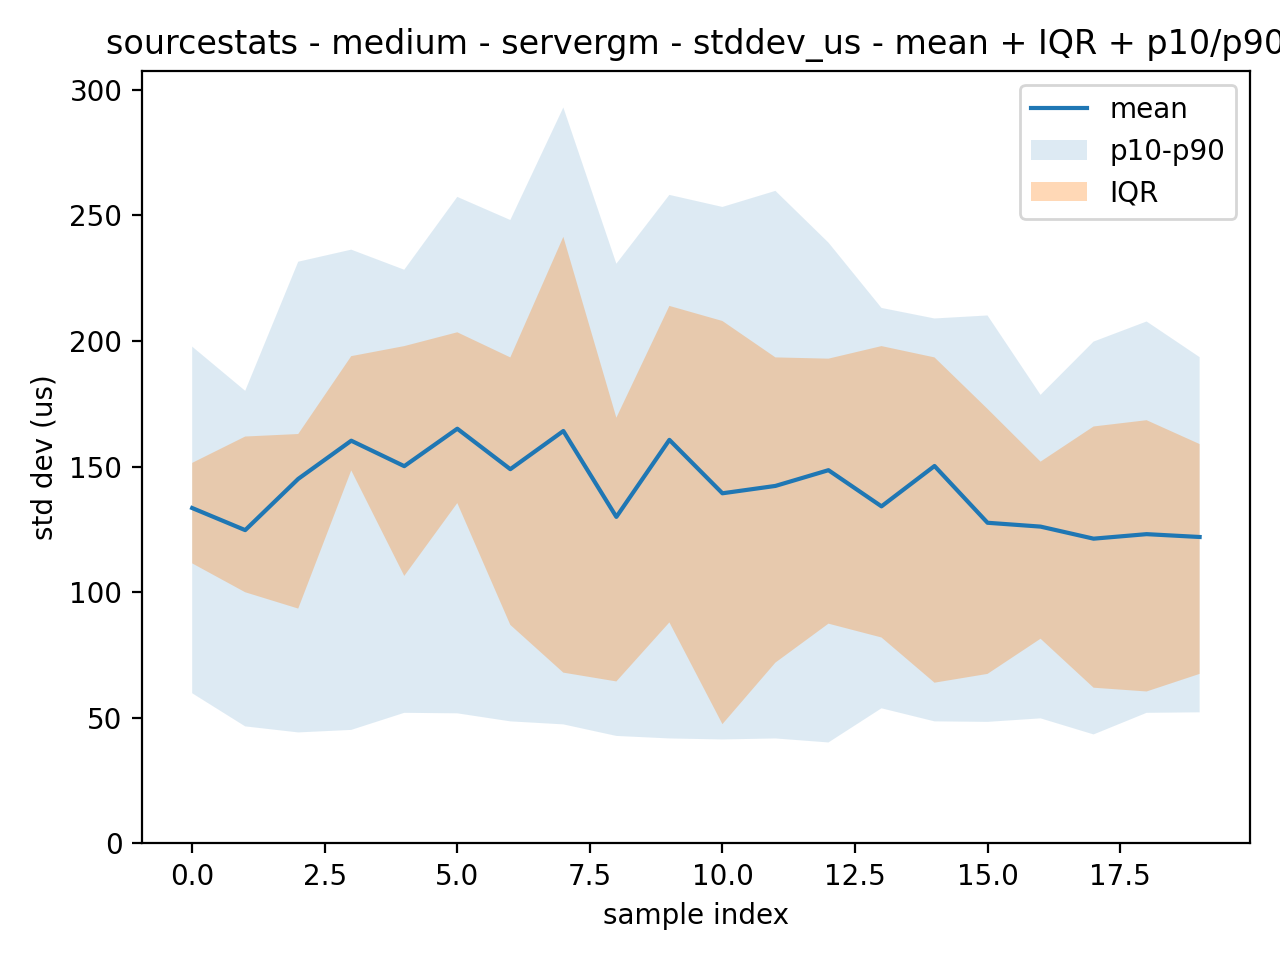
\includegraphics[width=\linewidth]{
      pars_plots/chrony_clientchrony/_aggregated/sourcestats/medium/servergm/stddev_us_mean_iqr_p10_p90.png
    }
    \caption{Scenario MEDIUM}
  \end{subfigure}
  \begin{subfigure}
    {0.32\textwidth}
    \centering
    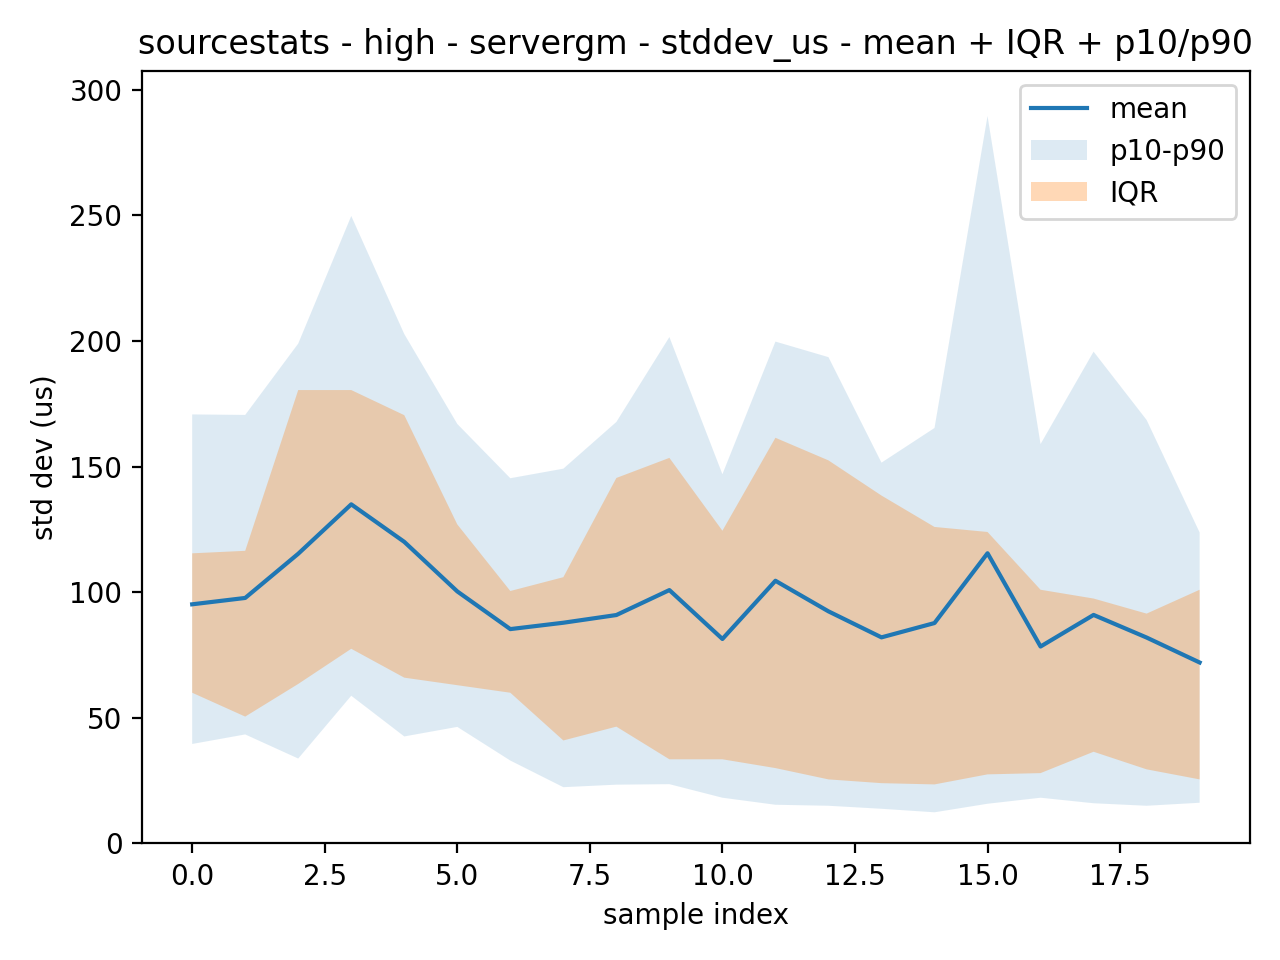
\includegraphics[width=\linewidth]{
      pars_plots/chrony_clientchrony/_aggregated/sourcestats/high/servergm/stddev_us_mean_iqr_p10_p90.png
    }
    \caption{Scenario HIGH}
  \end{subfigure}
  \caption{Media con banda inter-quartile e banda p10-p90 - nodo: \texttt{clientchrony}
  - netem/tc: \texttt{clientchrony}}
  \label{fig:scenario_comparison}
\end{figure}
\paragraph*{clientchrony - netem/tc:}
Per la metrica \texttt{stddev\_us}, il caso \texttt{clientchrony} non è presente una variazione
monotona crescente, ma piuttosto una risposta non lineare della variabilità
stimata rispetto alla sorgente. In tutti i casi i valori restano dell'ordine delle
centinaia di microsecondi.

Nello scenario \texttt{low} si ha una media aggregata di ~\texttt{109.552 \,$\mu$s}.
La dispersione non è trascurabile. La deviazione standard delle medie è di ~\texttt{21.838
\,$\mu$s}, in un intervallo d \texttt{78.637 \,$\mu$s} e \texttt{154.733 \,$\mu$s}.
Ci sono bande relativamente ampie, con IQR medio di ~\texttt{98.925 \,$\mu$s} e
ampiezza media \texttt{p10-p90} pari a \texttt{155.630 \,$\mu$s}. La mediana è ~\texttt{103
\,$\mu$s}, il terzo quartile \texttt{167 \,$\mu$s} e il massimo \texttt{464 \,$\mu$s}.

Nel caso \texttt{medium} si ha una crescita dei valori. La media aggregata è di
~\texttt{140.899 \,$\mu$s}. La mediana della curva è di ~\texttt{140.867 \,$\mu$s}
con valori che oscillano nell'intervallo \texttt{121.333 \,$\mu$s} e \texttt{165.109
\,$\mu$s}. La deviazione standard delle medie è \texttt{14.774 \,$\mu$s}. Le
bande di variabilità risultano tuttavia più larghe del caso \texttt{low}: l'IQR
medio sale a \texttt{100.000 \,$\mu$s} e l'ampiezza media \texttt{p10-p90}
raggiunge \texttt{178.740 \,$\mu$s}. Si ha un terzo quartile di\texttt{191.250
\,$\mu$s} e un massimo di \texttt{510 \,$\mu$s}.

Nello scenario \texttt{high} la media aggregata della curva è di ~\texttt{95.787
\,$\mu$s}, con mediana \texttt{91.687 \,$\mu$s}. L'IQR medio vale \texttt{88.450
\,$\mu$s}, mentre l'ampiezza media \texttt{p10-p90} è pari a \texttt{154.760 \,$\mu$s},
dunque molto vicina al caso \texttt{low} ma inferiore al caso \texttt{medium}. I dati
mostrano una riduzione del livello medio, con media complessiva \texttt{95.787
\,$\mu$s}, mediana \texttt{88 \,$\mu$s} e massimo \texttt{410 \,$\mu$s}.

Lo scenario \texttt{medium} è quello che presenta il livello medio più elevato,
\texttt{low} occupa una posizione intermedia e \texttt{high} mostra invece valori
medi più contenuti. Anche sul piano della dispersione intra-curva e inter-run non
si osserva una crescita progressiva con l'intensità del degrado. Pertanto, per questa
metrica, il degrado applicato su \texttt{clientchrony} non produce una risposta semplicemente
crescente, ma modifica la stima della deviazione standard in modo più articolato,
con un massimo nel caso \texttt{medium} e un successivo ridimensionamento nel
caso \texttt{high}.

\begin{figure}[H]
  \centering

  \begin{subfigure}
    {0.32\textwidth}
    \centering
    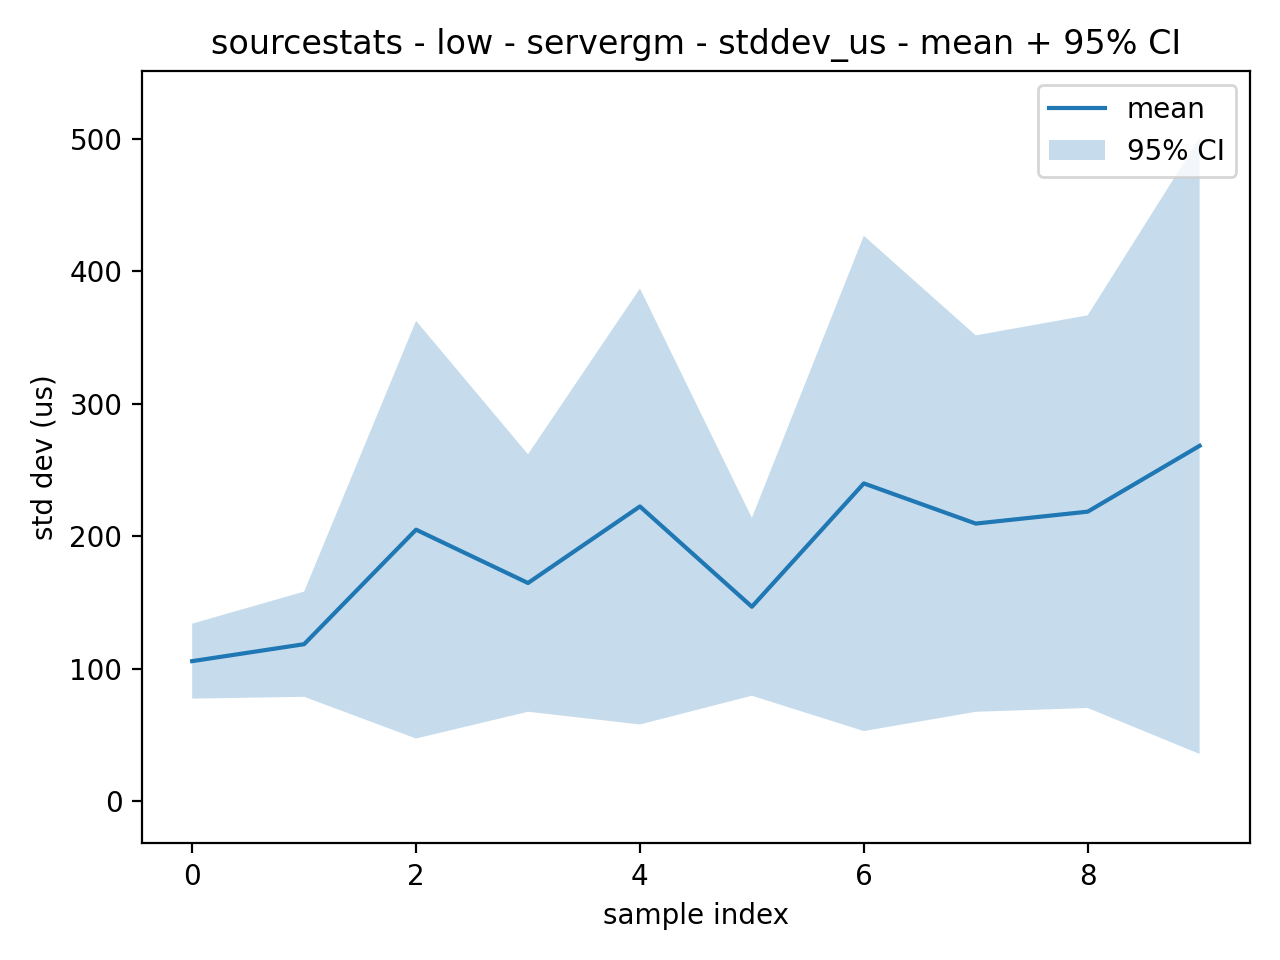
\includegraphics[width=\linewidth]{
      pars_plots/chrony_servergm/_aggregated/sourcestats/low/servergm/stddev_us_mean_ci95.png
    }
    \caption{Scenario LOW}
  \end{subfigure}
  \hfill
  \begin{subfigure}
    {0.32\textwidth}
    \centering
    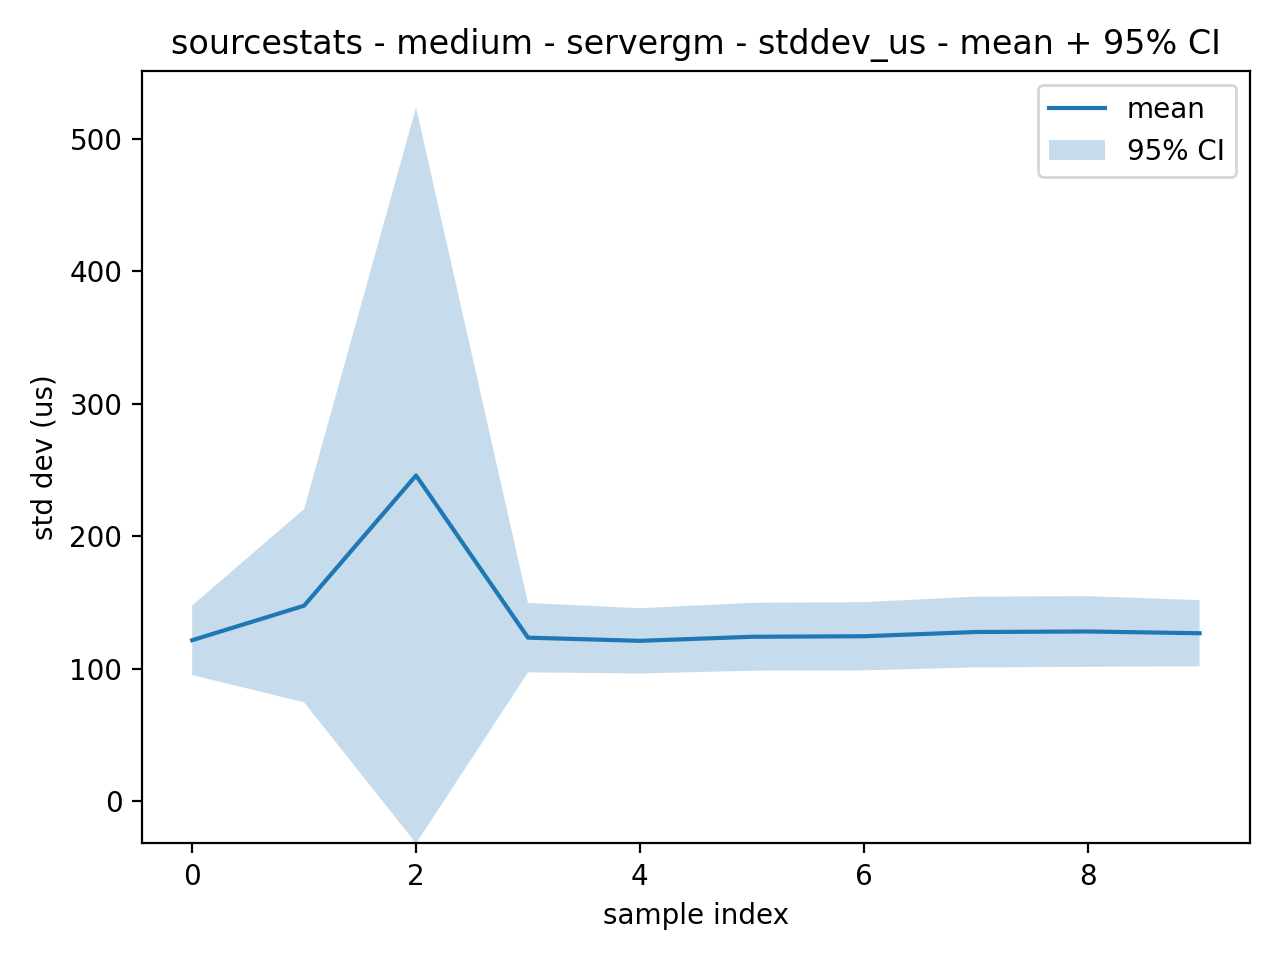
\includegraphics[width=\linewidth]{
      pars_plots/chrony_servergm/_aggregated/sourcestats/medium/servergm/stddev_us_mean_ci95.png
    }
    \caption{Scenario MEDIUM}
  \end{subfigure}
  \begin{subfigure}
    {0.32\textwidth}
    \centering
    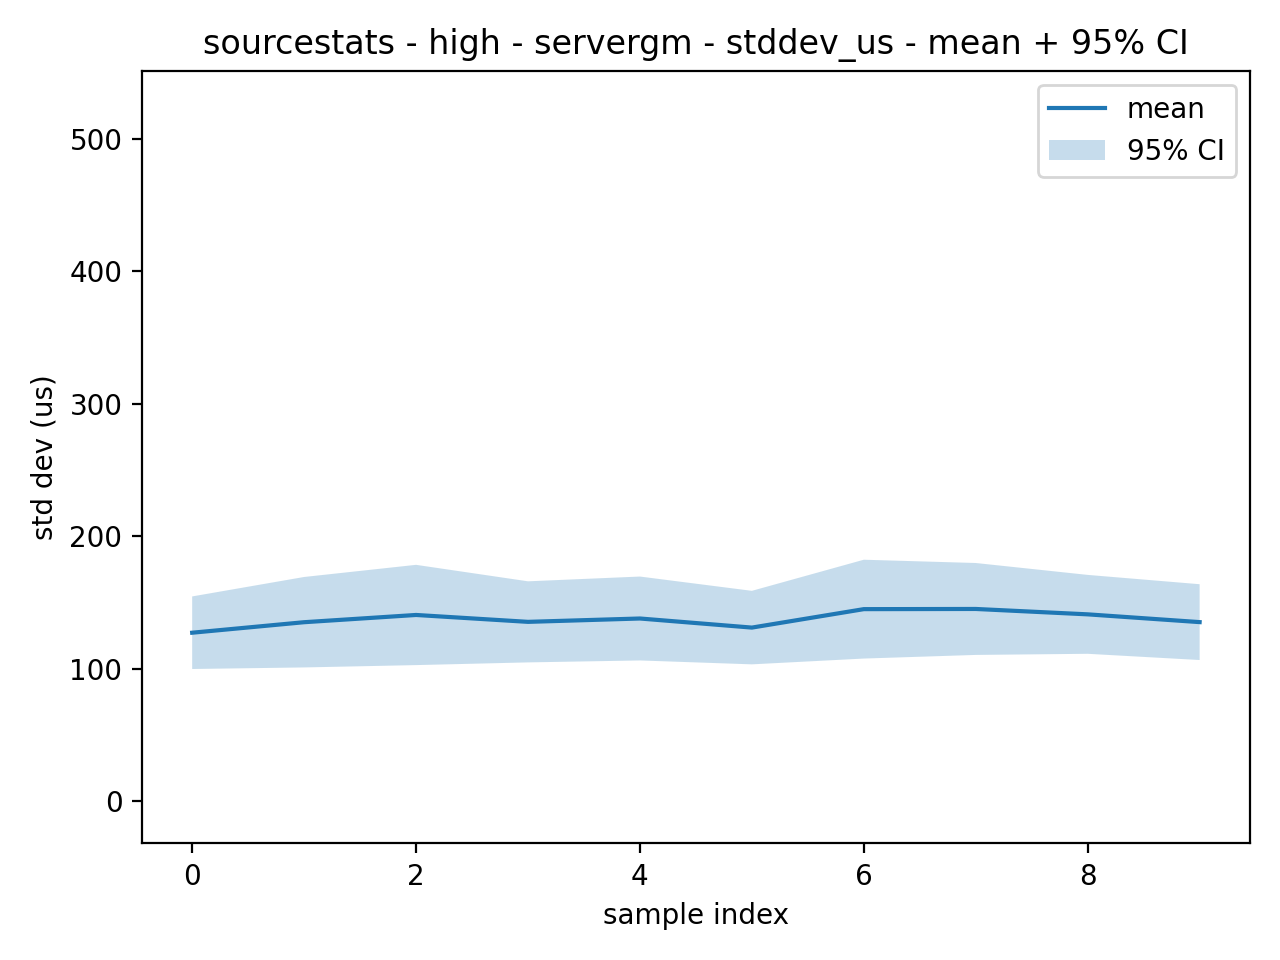
\includegraphics[width=\linewidth]{
      pars_plots/chrony_servergm/_aggregated/sourcestats/high/servergm/stddev_us_mean_ci95.png
    }
    \caption{Scenario HIGH}
  \end{subfigure}
  \caption{Media con intervallo di confidenza al 95\% - nodo: \texttt{clientchrony}
  - netem/tc: \texttt{servergm}}
  \label{fig:scenario_comparison}
\end{figure}
\begin{figure}[H]
  \centering

  \begin{subfigure}
    {0.32\textwidth}
    \centering
    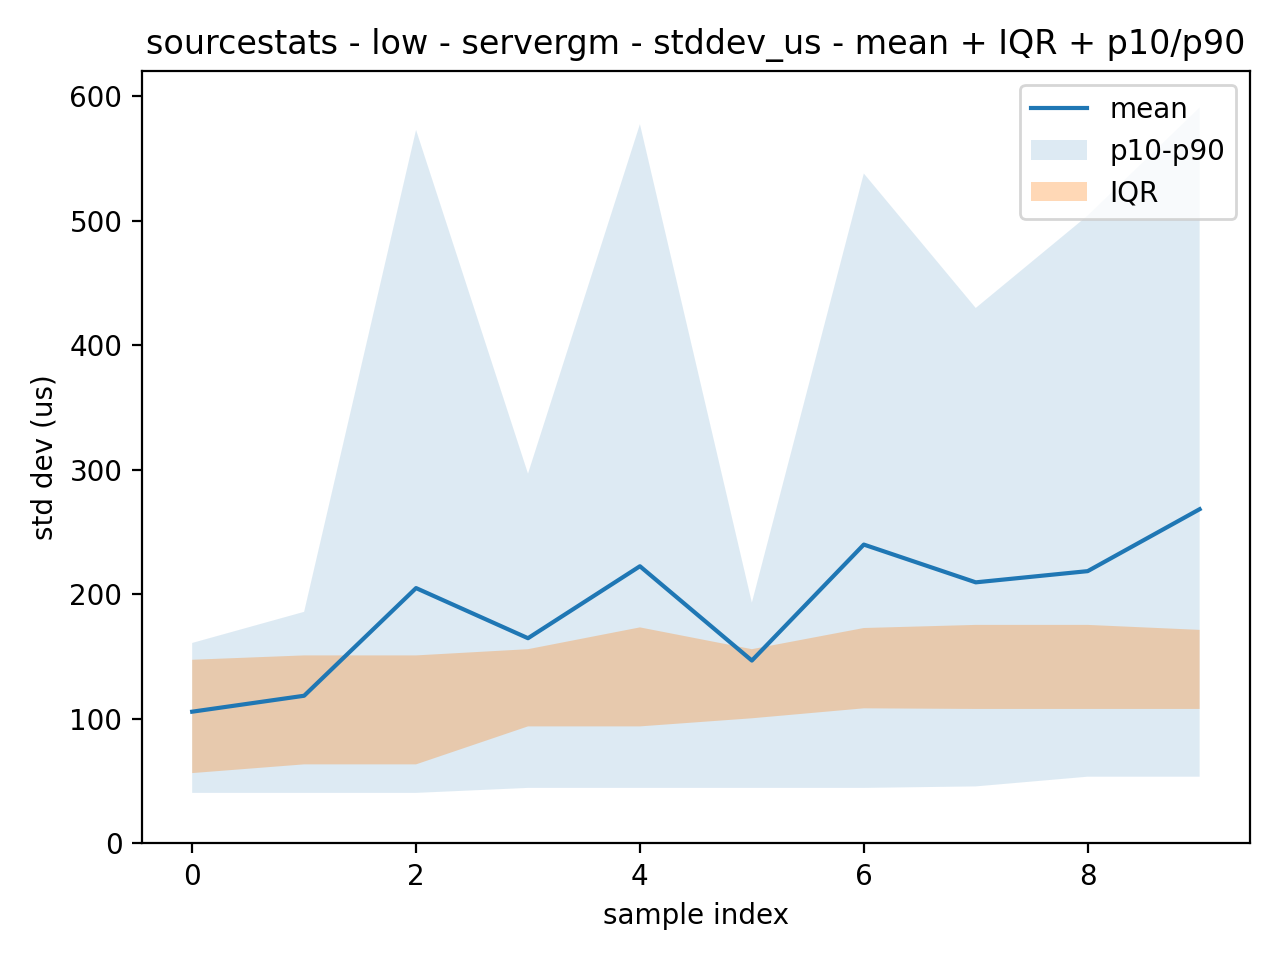
\includegraphics[width=\linewidth]{
      pars_plots/chrony_servergm/_aggregated/sourcestats/low/servergm/stddev_us_mean_iqr_p10_p90.png
    }
    \caption{Scenario LOW}
  \end{subfigure}
  \hfill
  \begin{subfigure}
    {0.32\textwidth}
    \centering
    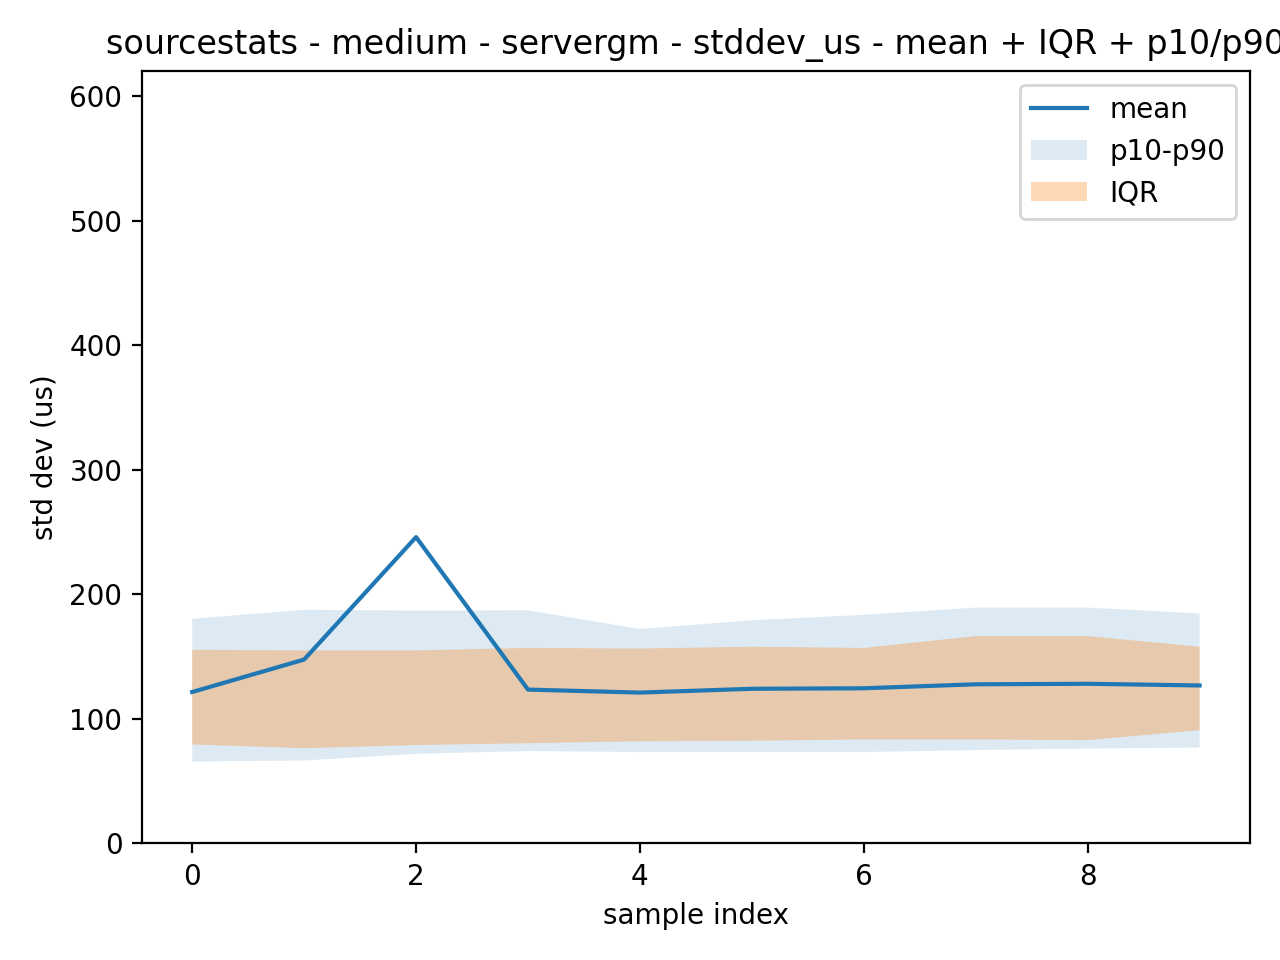
\includegraphics[width=\linewidth]{
      pars_plots/chrony_servergm/_aggregated/sourcestats/medium/servergm/stddev_us_mean_iqr_p10_p90.png
    }
    \caption{Scenario MEDIUM}
  \end{subfigure}
  \begin{subfigure}
    {0.32\textwidth}
    \centering
    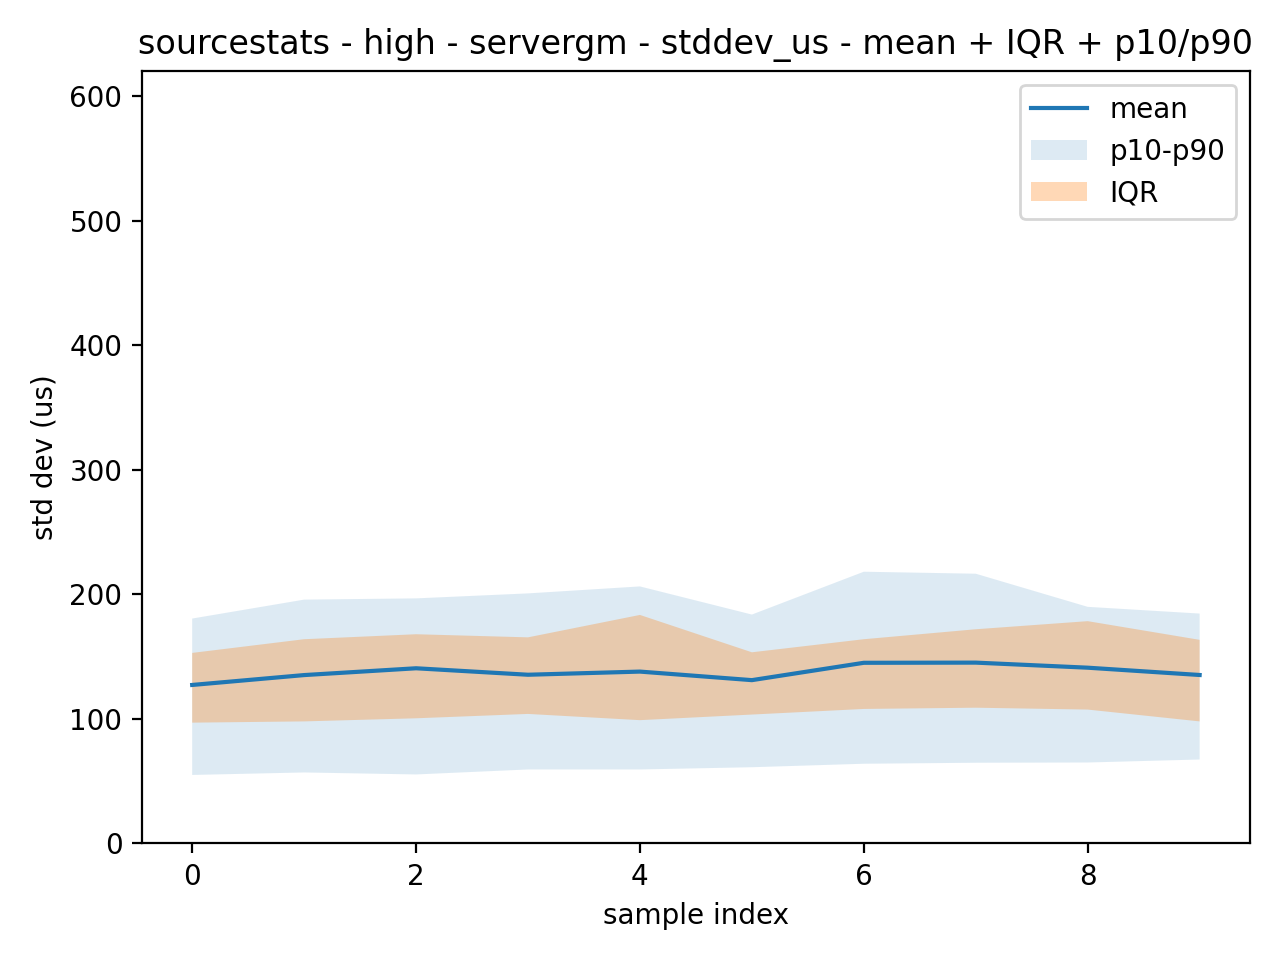
\includegraphics[width=\linewidth]{
      pars_plots/chrony_servergm/_aggregated/sourcestats/high/servergm/stddev_us_mean_iqr_p10_p90.png
    }
    \caption{Scenario HIGH}
  \end{subfigure}
  \caption{Media con banda inter-quartile e banda p10-p90 - nodo: \texttt{clientchrony}
  - netem/tc: \texttt{servergm}}
  \label{fig:scenario_comparison}
\end{figure}

\paragraph*{servergm - netem/tc:}
Nello scenario \texttt{low} la media aggregata è \texttt{190.047 \,$\mu$s} e la deviazione
standard delle medie è di \texttt{53.570 \,$\mu$s}. L'IQR medio è di \texttt{72.600
\,$\mu$s}, e l'ampiezza media dell'intervallo \texttt{p10-p90} raggiunge \texttt{359.800
\,$\mu$s}, con picchi fino a \texttt{537.400 \,$\mu$s}. Si ha un massimo di
\texttt{1622 \,$\mu$s}. Nel complesso, quindi, lo scenario \texttt{low} descrive una
stima della deviazione standard elevata e accompagnata da una variabilità molto marcata
tra le run. In tale scenario, la media è più affetta dagli outlier che dai valori tipici, 
si nota dalla presenza di un valore medio che si discosta dalla banda inter-quartile.

Nel caso \texttt{medium} la media aggregata della curva è di \texttt{139.160 \,$\mu$s}.
La deviazione standard delle medie è di \texttt{38.298 \,$\mu$s}. I valori medi
risultano compresi tra \texttt{121.133 \,$\mu$s} e \texttt{246.000 \,$\mu$s}. L'IQR
medio vale \texttt{76.400 \,$\mu$s}, mentre l'intervallo medio \texttt{p10-p90}
è pari a \texttt{111.360 \,$\mu$s}. Si ha una mediana di \texttt{130 \,$\mu$s}.
Il massimo pari a \texttt{2053 \,$\mu$s}

Nello scenario \texttt{high} la media aggregata è pari a \texttt{137.440 \,$\mu$s}.
La deviazione standard delle medie scende drasticamente a \texttt{5.770 \,$\mu$s}.
Anche l'intervallo dei valori medi lungo la curva risulta molto ristretto,
compreso tra \texttt{127.267 \,$\mu$s} e \texttt{145.200 \,$\mu$s}. Le bande di dispersione
si contraggono: l'IQR medio è pari a \texttt{64.100 \,$\mu$s} e l'ampiezza media \texttt{p10-p90}
è \texttt{136.500 \,$\mu$s}.

Non è presente una dinamica lineare nel confronto. Il caso \texttt{low} la maggiore
dispersione. I casi \texttt{medium} e \texttt{high} mostrano invece medie
inferiori e molto simili tra loro, ma differiscono sul piano della stabilità.

\paragraph*{Confronto:}
L'impairment sul server tende a produrre un effetto più severo soprattutto nel
caso \texttt{low}, accompagnato da una dispersione molto marcata e da outlier
più pronunciati. L'impairment sul client mostra invece un comportamento più regolare,
con variazioni meno estreme e una risposta non monotona centrata sul caso
\texttt{medium}.

\subsection{Analisi metrica: \texttt{system time offset}}
\begin{figure}[H]
  \centering

  \begin{subfigure}
    {0.32\textwidth}
    \centering
    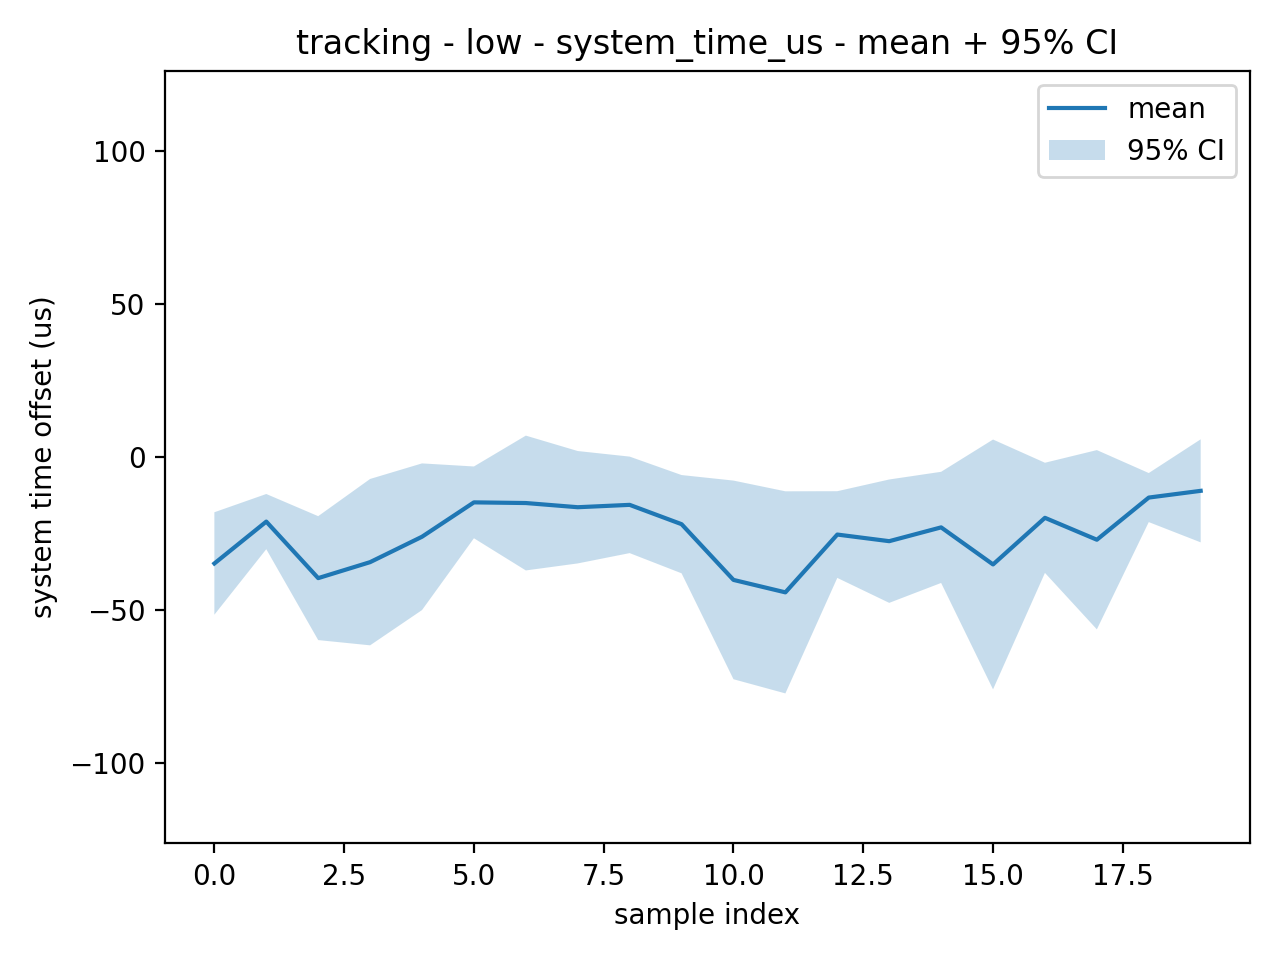
\includegraphics[width=\linewidth]{
      pars_plots/chrony_clientchrony/_aggregated/tracking/low/system_time_us_mean_ci95.png
    }
    \caption{Scenario LOW}
  \end{subfigure}
  \hfill
  \begin{subfigure}
    {0.32\textwidth}
    \centering
    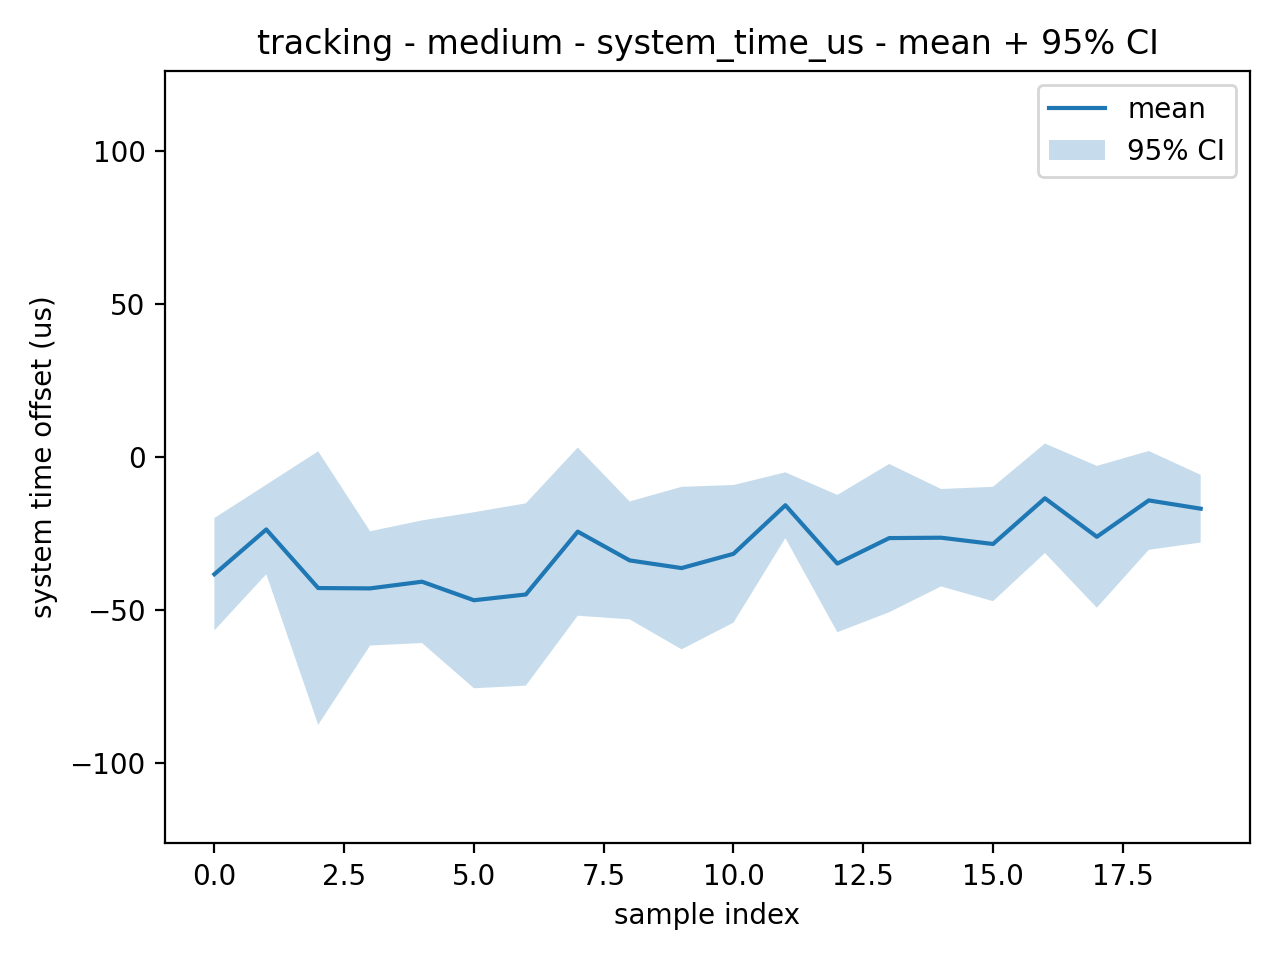
\includegraphics[width=\linewidth]{
      pars_plots/chrony_clientchrony/_aggregated/tracking/medium/system_time_us_mean_ci95.png
    }
    \caption{Scenario MEDIUM}
  \end{subfigure}
  \begin{subfigure}
    {0.32\textwidth}
    \centering
    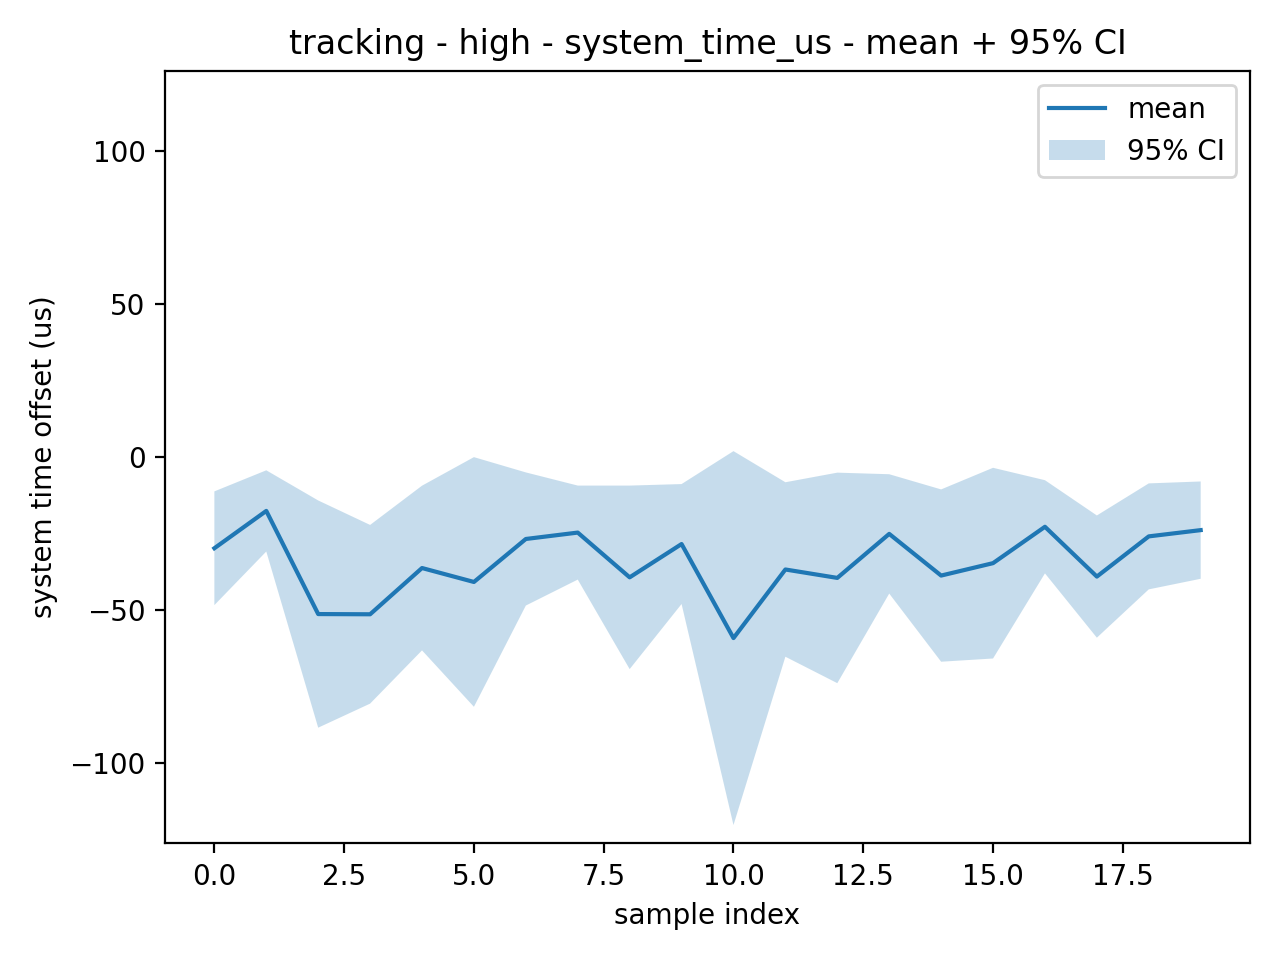
\includegraphics[width=\linewidth]{
      pars_plots/chrony_clientchrony/_aggregated/tracking/high/system_time_us_mean_ci95.png
    }
    \caption{Scenario HIGH}
  \end{subfigure}
  \caption{Media con intervallo di confidenza al 95\% - nodo: \texttt{clientchrony}
  - netem/tc: \texttt{clientchrony}}
  \label{fig:scenario_comparison}
\end{figure}
\begin{figure}[H]
  \centering

  \begin{subfigure}
    {0.32\textwidth}
    \centering
    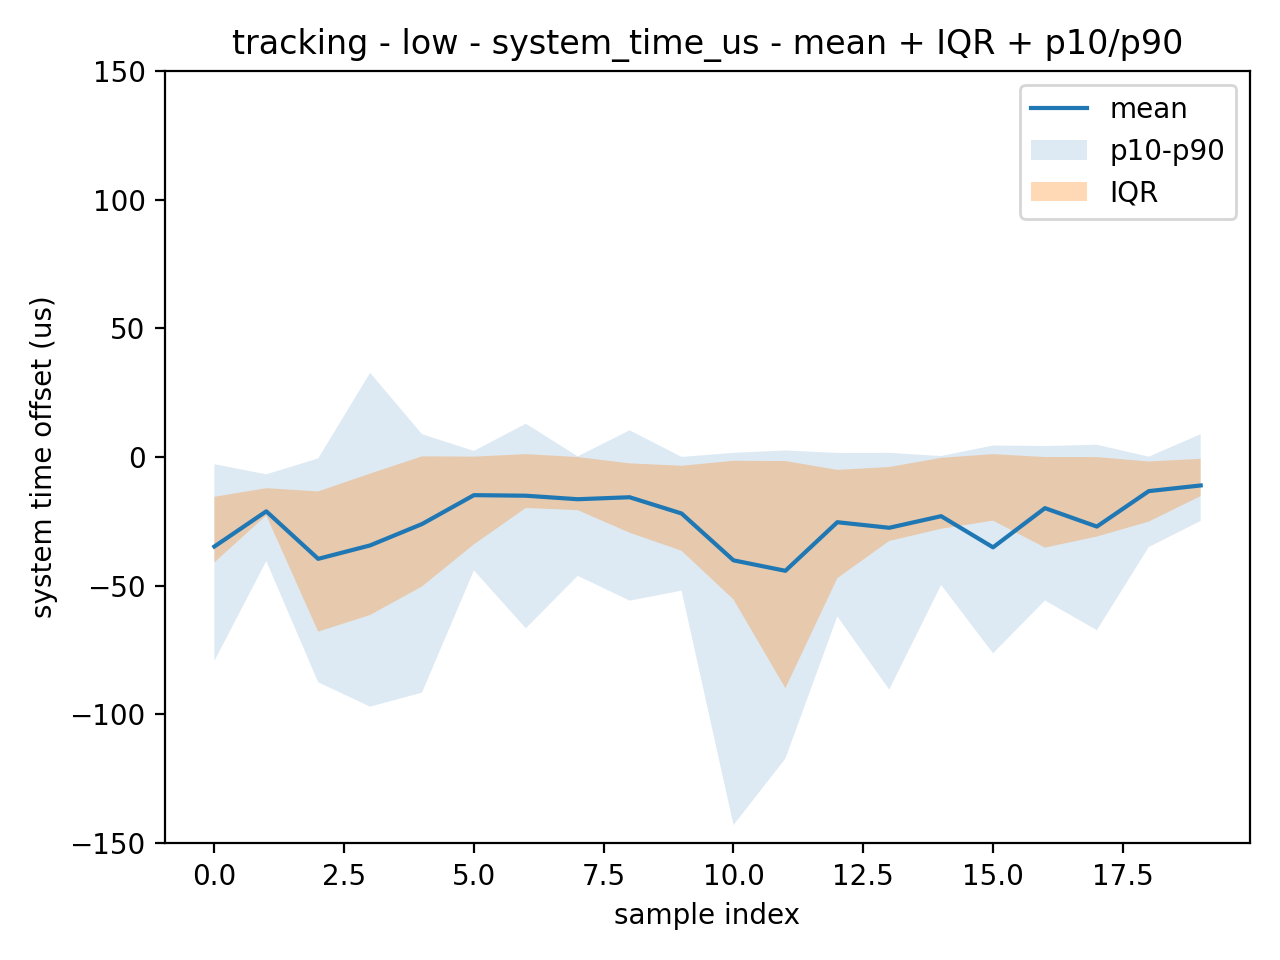
\includegraphics[width=\linewidth]{
      pars_plots/chrony_clientchrony/_aggregated/tracking/low/system_time_us_mean_iqr_p10_p90.png
    }
    \caption{Scenario LOW}
  \end{subfigure}
  \hfill
  \begin{subfigure}
    {0.32\textwidth}
    \centering
    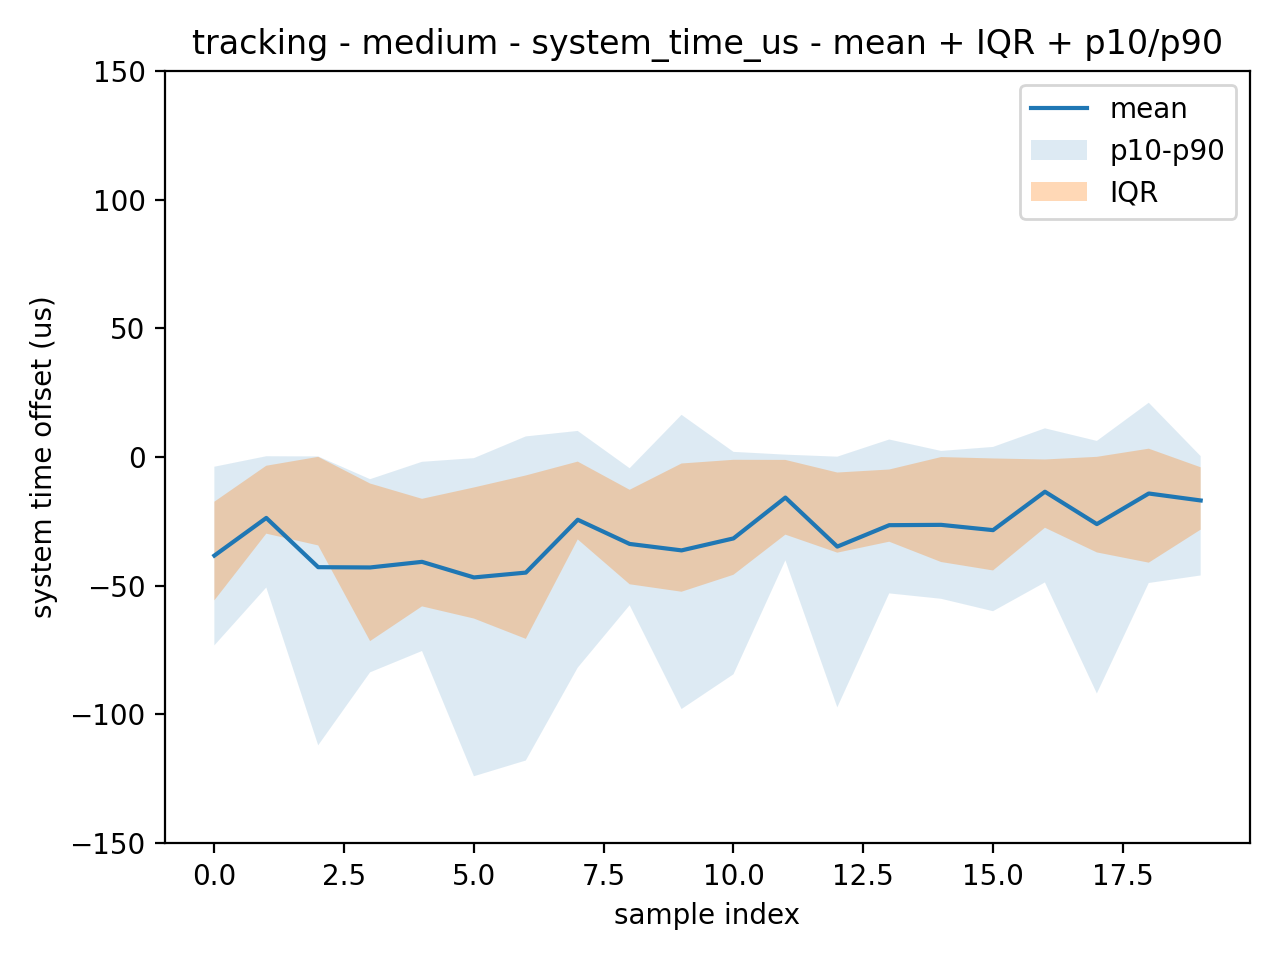
\includegraphics[width=\linewidth]{
      pars_plots/chrony_clientchrony/_aggregated/tracking/medium/system_time_us_mean_iqr_p10_p90.png
    }
    \caption{Scenario MEDIUM}
  \end{subfigure}
  \begin{subfigure}
    {0.32\textwidth}
    \centering
    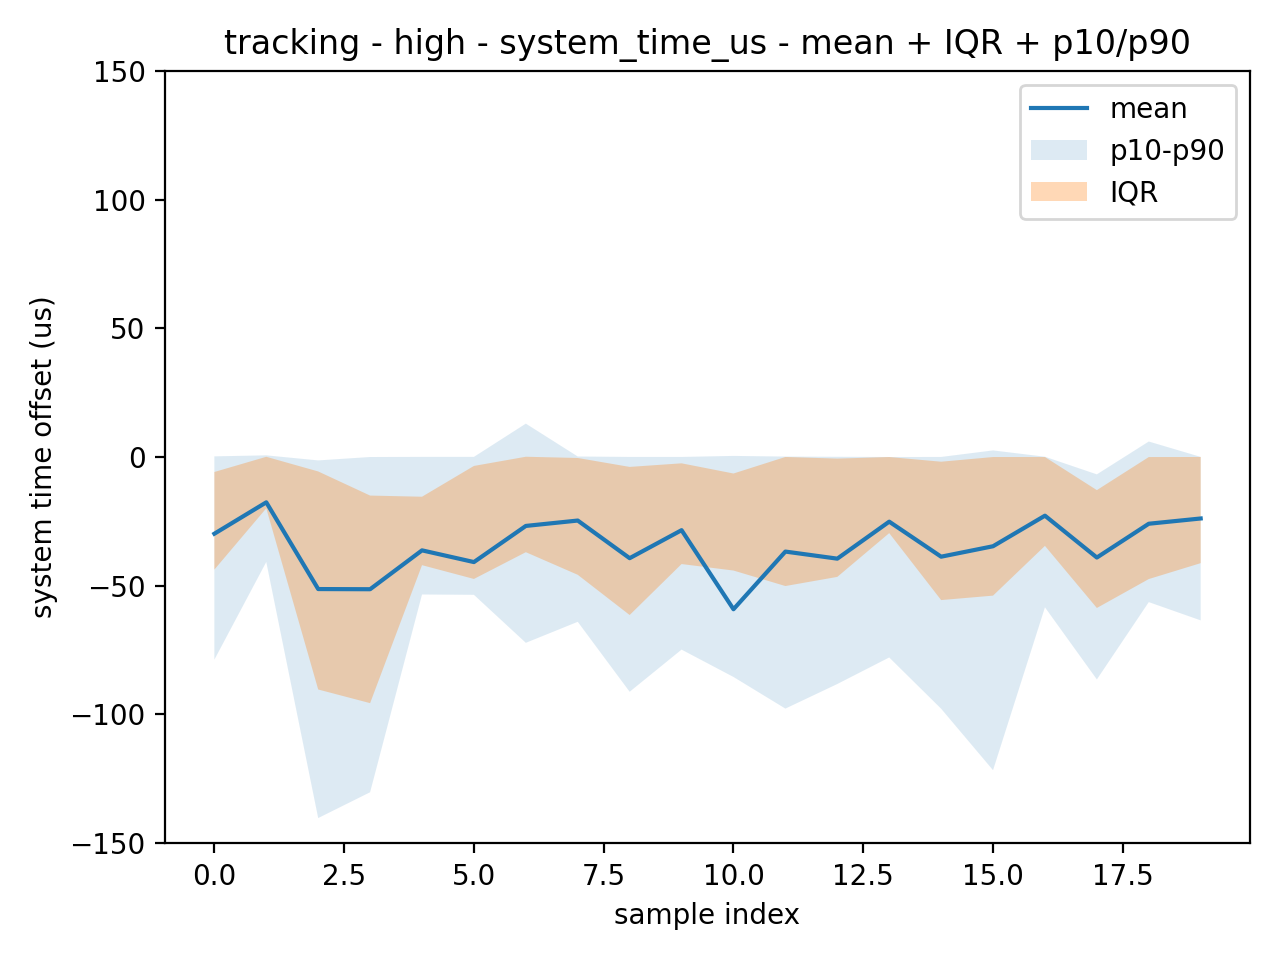
\includegraphics[width=\linewidth]{
      pars_plots/chrony_clientchrony/_aggregated/tracking/high/system_time_us_mean_iqr_p10_p90.png
    }
    \caption{Scenario HIGH}
  \end{subfigure}
  \caption{Media con banda inter-quartile e banda p10-p90 - nodo: \texttt{clientchrony}
  - netem/tc: \texttt{clientchrony}}
  \label{fig:scenario_comparison}
\end{figure}
\paragraph*{clientchrony - netem/tc:}
Nel caso della metrica \texttt{system\_time\_us}, l'analisi relativa a \texttt{clientchrony}
con degrado applicato sul nodo client evidenzia un comportamento più regolare rispetto
ad altre metriche.

Nel caso \texttt{low} la media aggregata è di ~\texttt{-25.284 \,$\mu$s}. La deviazione
standard delle medie è di \texttt{9.885 \,$\mu$s}. I grafici evidenziano oscillazioni
locali. L'IQR medio è pari a \texttt{35.089 \,$\mu$s}. L'ampiezza media dell'intervallo
\texttt{p10-p90} raggiunge \texttt{73.456 \,$\mu$s}, con picchi fino a \texttt{144.596
\,$\mu$s}. Nei dati globali si ha una mediana \texttt{-13.664 \,$\mu$s}, primo quartile
\texttt{-34.557 \,$\mu$s} e terzo quartile \texttt{-0.530 \,$\mu$s}.

Nello scenario \texttt{medium} la media aggregata della curva scende a \texttt{-30.408
\,$\mu$s}. La deviazione standard delle medie pari a \texttt{10.531 \,$\mu$s}. L'IQR
medio vale \texttt{39.129 \,$\mu$s}, mentre l'intervallo medio \texttt{p10-p90} è
\texttt{78.520 \,$\mu$s}. Le statistiche globali hanno mediana \texttt{-22.285 \,$\mu$s}
e quartili pari a \texttt{-46.666 \,$\mu$s} e \texttt{-2.351 \,$\mu$s}.

Nello scenario \texttt{high} la media aggregata della curva è di \texttt{-34.573 \,$\mu$s},
il valore più negativo tra i tre scenari. La deviazione standard delle medie è
\texttt{10.809 \,$\mu$s}. L'IQR medio è \texttt{45.637 \,$\mu$s} e l'ampiezza media
\texttt{p10-p90} è \texttt{82.403 \,$\mu$s}. Si ha mediana pari a\texttt{-19.111 \,$\mu$s},
primo quartile \texttt{-48.642 \,$\mu$s} e terzo quartile \texttt{0.001 \,$\mu$s}.

Nel confronto complessivo tra i tre scenari emerge quindi una dinamica lineare.
Il passaggio da \texttt{low} a \texttt{medium} e poi a \texttt{high} produce infatti
un progressivo spostamento del livello medio verso valori più negativi: \texttt{-25.284
\,$\mu$s}, \texttt{-30.408 \,$\mu$s} e \texttt{-34.573 \,$\mu$s}. La variabilità rimane
ampia in tutti e tre i casi e non cresce in modo altrettanto netto.

\begin{figure}[H]
  \centering

  \begin{subfigure}
    {0.32\textwidth}
    \centering
    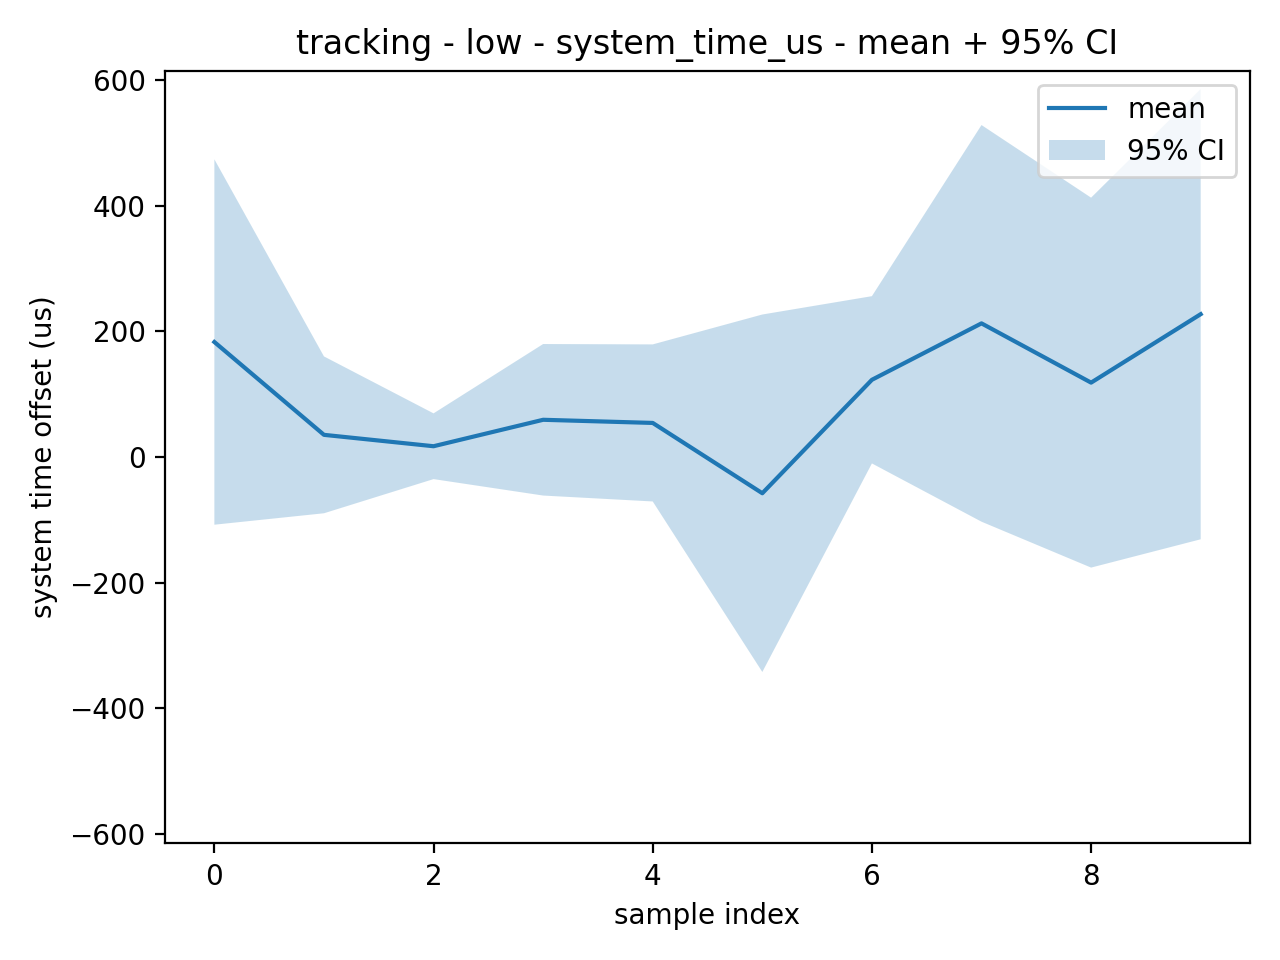
\includegraphics[width=\linewidth]{
      pars_plots/chrony_servergm/_aggregated/tracking/low/system_time_us_mean_ci95.png
    }
    \caption{Scenario LOW}
  \end{subfigure}
  \hfill
  \begin{subfigure}
    {0.32\textwidth}
    \centering
    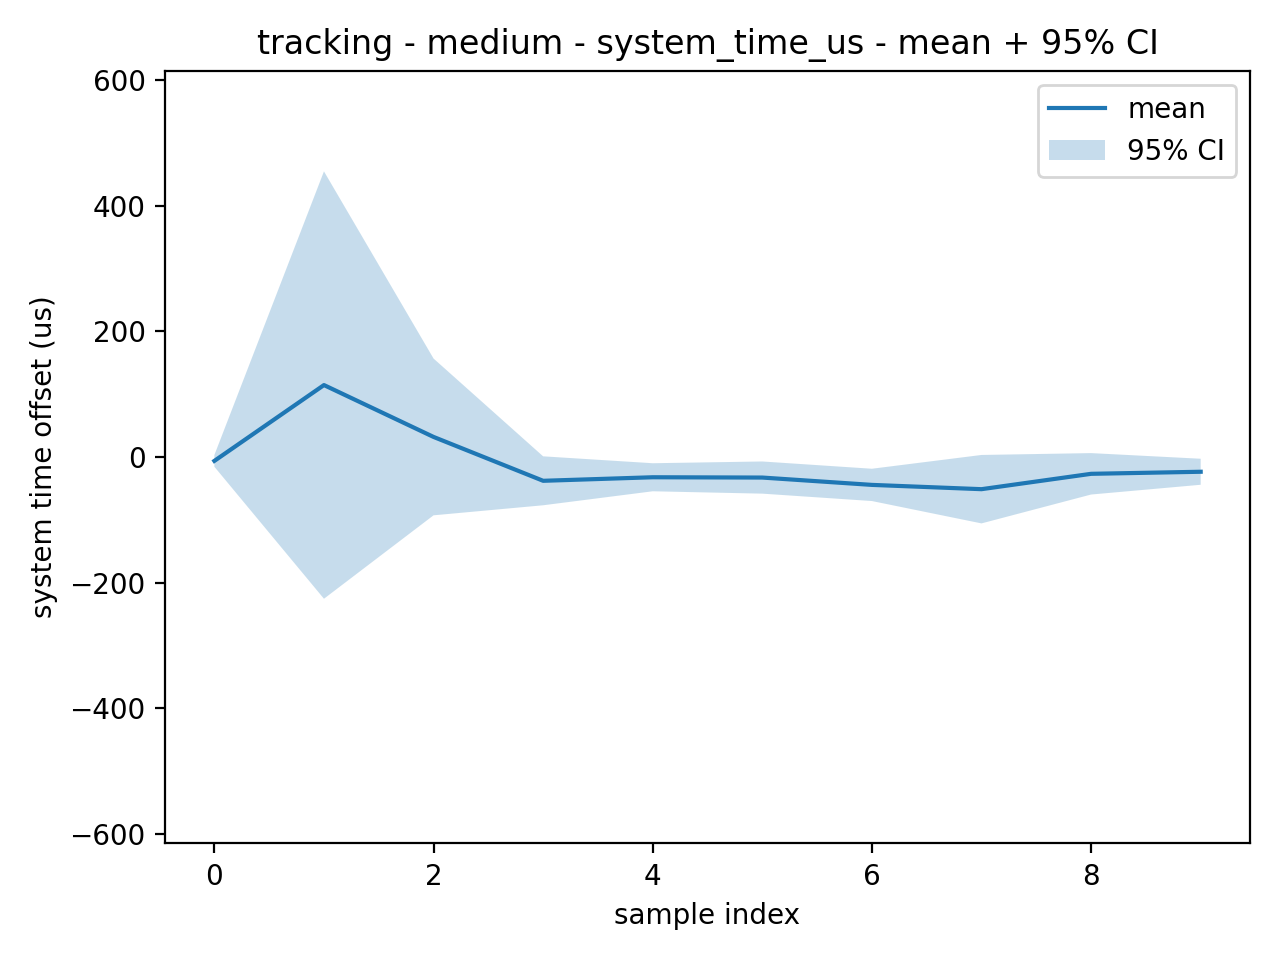
\includegraphics[width=\linewidth]{
      pars_plots/chrony_servergm/_aggregated/tracking/medium/system_time_us_mean_ci95.png
    }
    \caption{Scenario MEDIUM}
  \end{subfigure}
  \begin{subfigure}
    {0.32\textwidth}
    \centering
    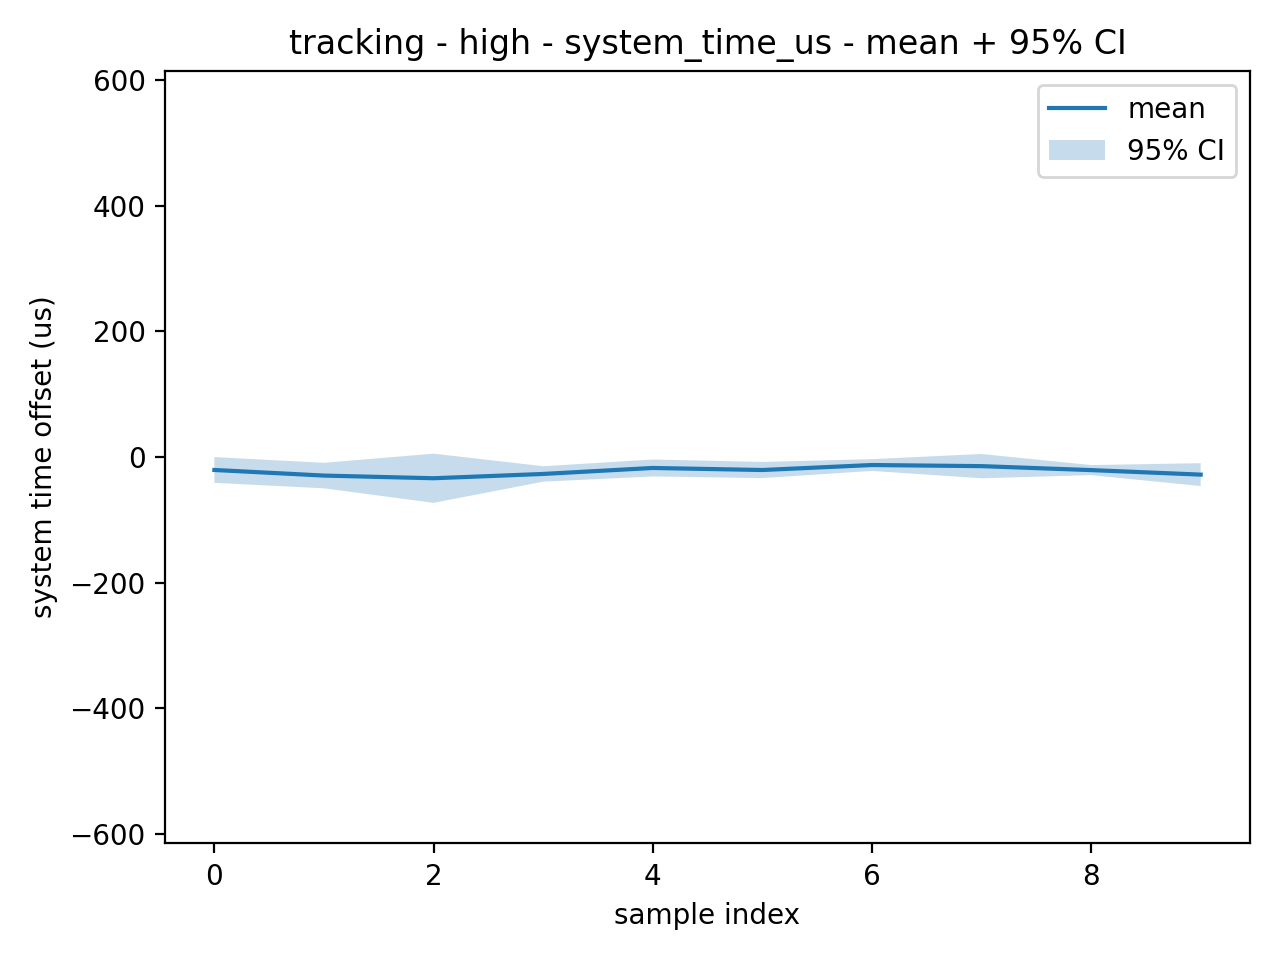
\includegraphics[width=\linewidth]{
      pars_plots/chrony_servergm/_aggregated/tracking/high/system_time_us_mean_ci95.png
    }
    \caption{Scenario HIGH}
  \end{subfigure}
  \caption{Media con intervallo di confidenza al 95\% - nodo: \texttt{clientchrony}
  - netem/tc: \texttt{servergm}}
  \label{fig:scenario_comparison}
\end{figure}
\begin{figure}[H]
  \centering

  \begin{subfigure}
    {0.32\textwidth}
    \centering
    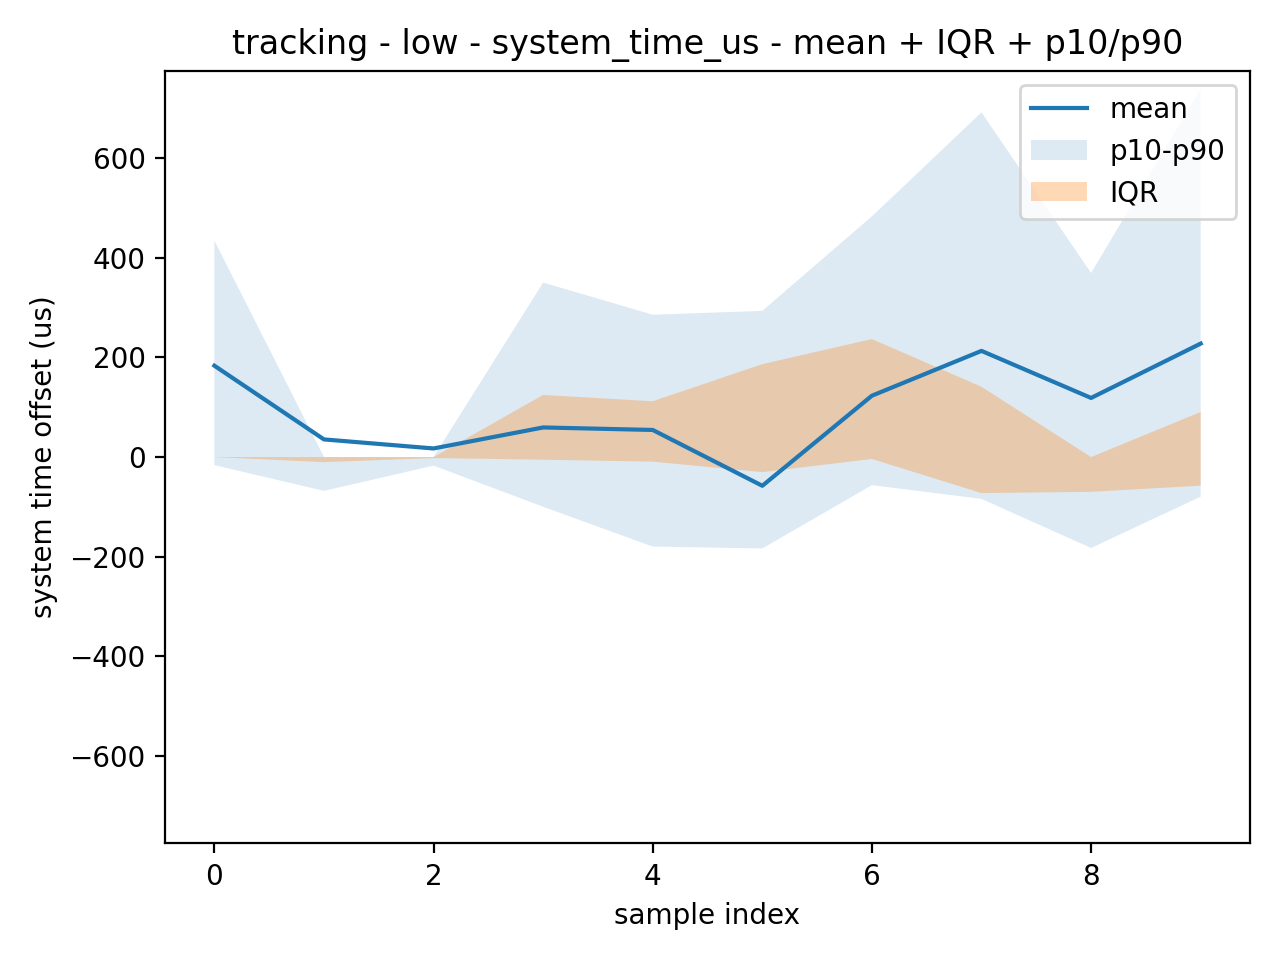
\includegraphics[width=\linewidth]{
      pars_plots/chrony_servergm/_aggregated/tracking/low/system_time_us_mean_iqr_p10_p90.png
    }
    \caption{Scenario LOW}
  \end{subfigure}
  \hfill
  \begin{subfigure}
    {0.32\textwidth}
    \centering
    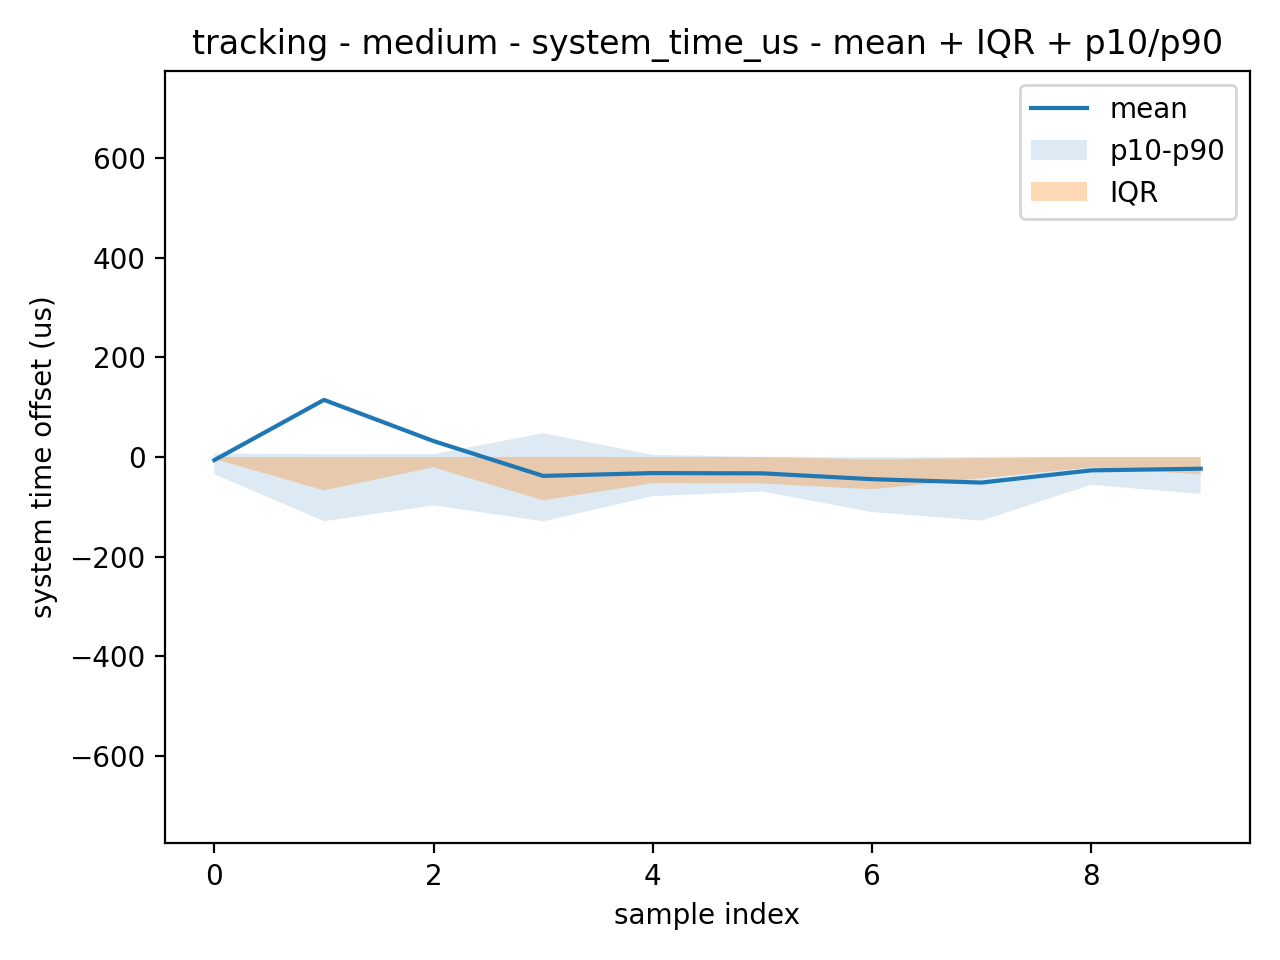
\includegraphics[width=\linewidth]{
      pars_plots/chrony_servergm/_aggregated/tracking/medium/system_time_us_mean_iqr_p10_p90.png
    }
    \caption{Scenario MEDIUM}
  \end{subfigure}
  \begin{subfigure}
    {0.32\textwidth}
    \centering
    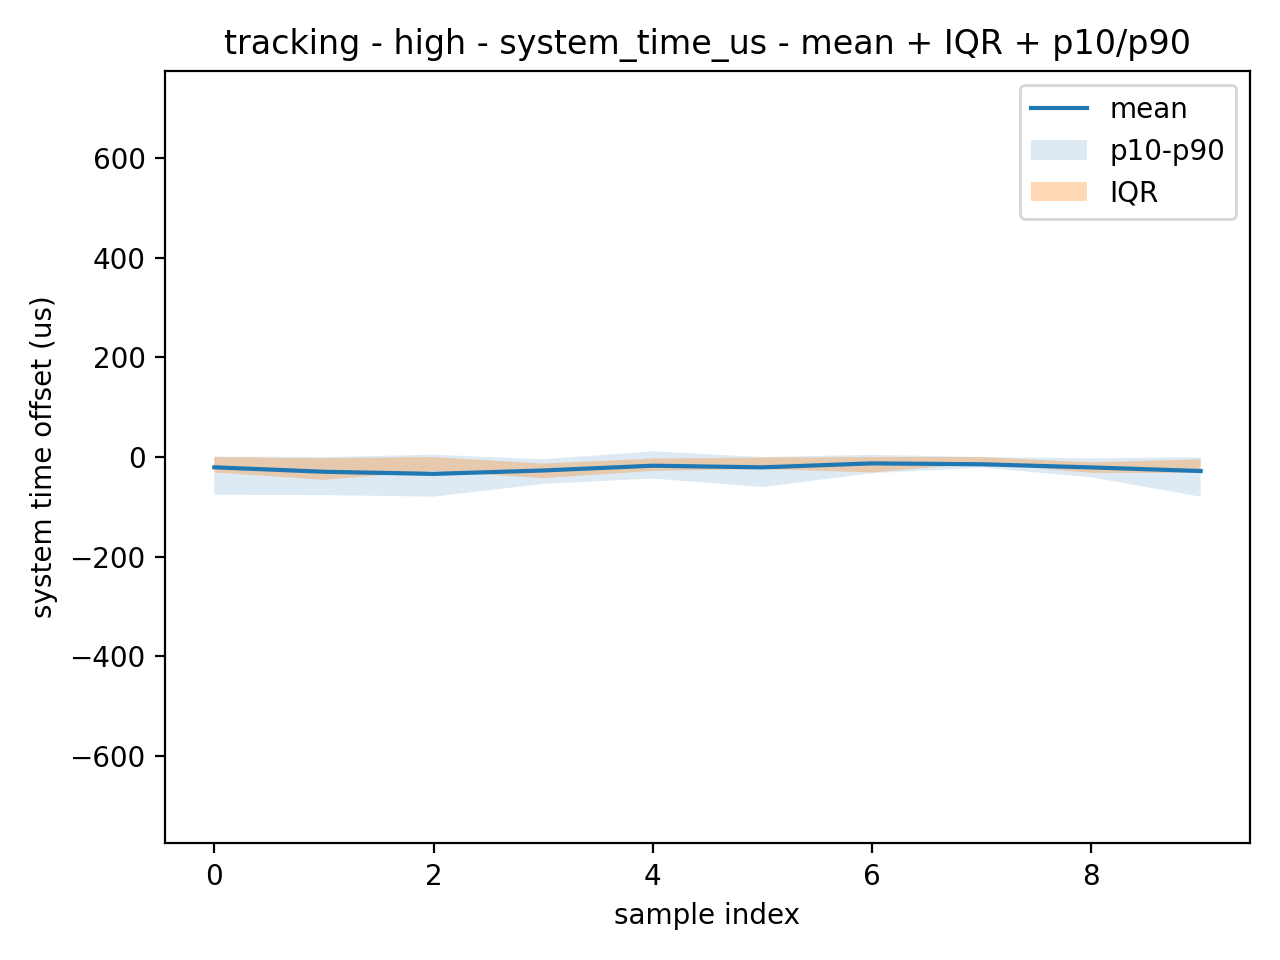
\includegraphics[width=\linewidth]{
      pars_plots/chrony_servergm/_aggregated/tracking/high/system_time_us_mean_iqr_p10_p90.png
    }
    \caption{Scenario HIGH}
  \end{subfigure}
  \caption{Media con banda inter-quartile e banda p10-p90 - nodo: \texttt{clientchrony}
  - netem/tc: \texttt{servergm}}
  \label{fig:scenario_comparison}
\end{figure}

\paragraph*{servergm - netem/tc:}
L'analisi con impairment applicato sul nodo \texttt{servergm} evidenzia un
comportamento fortemente non monotono al variare dello scenario.

Nello scenario \texttt{low}, la metrica assume il livello medio più elevato. La media
aggregata della curva è pari a \texttt{97.407 \,$\mu$s}. La deviazione standard delle
medie pari a \texttt{92.121 \,$\mu$s}. L'IQR medio è \texttt{115.127 \,$\mu$s}, mentre
l'ampiezza media dell'intervallo \texttt{p10-p90} raggiunge \texttt{461.010 \,$\mu$s},
con picchi fino a \texttt{817.440 \,$\mu$s}. Si ha un valore massimo pari a
\texttt{2342.321 \,$\mu$s}.Il caso \texttt{low} descrive quindi una risposta
molto instabile. È evidente la presenza di una media non congrua alle bande inter-quartile
per la maggior parte della run.

Nello scenario \texttt{medium}, la media aggregata della curva scende a \texttt{-10.765
\,$\mu$s}. La deviazione standard delle medie si riduce a \texttt{49.927 \,$\mu$s},
circa la metà del valore osservato nel caso \texttt{low}. L'IQR medio è pari a
\texttt{43.947 \,$\mu$s} e l'intervallo medio \texttt{p10-p90} vale \texttt{97.563
\,$\mu$s}. La mediana è di \texttt{-7.355 \,$\mu$s} e i quartili sono pari a \texttt{-50.338
\,$\mu$s} e \texttt{0.031 \,$\mu$s}.

Nello scenario \texttt{high}, la metrica mostra il comportamento più compatto e regolare.
La media aggregata della curva è pari a \texttt{-22.466 \,$\mu$s}, quindi più
negativa rispetto al caso \texttt{medium}, ma accompagnata da una deviazione
standard delle medie molto contenuta, pari a soli \texttt{6.852 \,$\mu$s}.L'IQR
medio è \texttt{27.040 \,$\mu$s}, mentre l'ampiezza media \texttt{p10-p90} è \texttt{57.641
\,$\mu$s}, entrambe inferiori ai valori osservati negli altri due scenari.

Nel confronto vi è un rapporto non lineare. Lo scenario \texttt{low} è nettamente
il più disperso e presenta anche il livello medio più elevato, positivo e
influenzato da run molto anomale. Lo scenario \texttt{medium} riduce
drasticamente tale effetto. Lo scenario \texttt{high} accentua ulteriormente
questa stabilizzazione. Il degrado applicato sul nodo \texttt{servergm} non
produce un peggioramento progressivo all'aumentare dello scenario

\paragraph*{Confronto:}
Nel confronto tra i due punti di applicazione del degrado non emerge una
superiorità univoca di uno scenario rispetto all'altro.